% ******************************* PhD Thesis Template **************************
% Please have a look at the README.md file for info on how to use the template

\documentclass[a4paper,12pt,customfont,numbered,print,index]{Classes/PhDThesisPSnPDF}

% ******************************************************************************
% ******************************* Class Options ********************************
% *********************** See README for more details **************************
% ******************************************************************************

% `a4paper'(The University of Cambridge PhD thesis guidelines recommends a page
% size a4 - default option) or `a5paper': A5 Paper size is also allowed as per
% the Cambridge University Engineering Deparment guidelines for PhD thesis
%
% `11pt' or `12pt'(default): Font Size 10pt is NOT recommended by the University
% guidelines
%
% `oneside' or `twoside'(default): Printing double side (twoside) or single
% side.
%
% `print': Use `print' for print version with appropriate margins and page
% layout. Leaving the options field blank will activate Online version.
%
% `index': For index at the end of the thesis
%
% `draftclassic': For draft mode without loading any images (same as draft in book)
%
% `draft': Special draft mode with line numbers, images, and water mark with
% timestamp and custom text. Position of the text can also be modified.
%
% `abstract': To generate only the title page and abstract page with
% dissertation title and name, to submit to the Student Registry
%
% `chapter`: This option enables only the specified chapter and it's references
%  Useful for review and corrections.
%
% ************************* Custom Page Margins ********************************
%
% `custommargin`: Use `custommargin' in options to activate custom page margins,
% which can be defined in the preamble.tex. Custom margin will override
% print/online margin setup.
%
% *********************** Choosing the Fonts in Class Options ******************
%
% `times' : Times font with math support. (The Cambridge University guidelines
% recommend using times)
%
% `fourier': Utopia Font with Fourier Math font (Font has to be installed)
%            It's a free font.
%
% `customfont': Use `customfont' option in the document class and load the
% package in the preamble.tex
%
% default or leave empty: `Latin Modern' font will be loaded.
%
% ********************** Choosing the Bibliography style ***********************
%
% `authoryear': For author-year citation eg., Krishna (2013)
%
% `numbered': (Default Option) For numbered and sorted citation e.g., [1,5,2]
%
% `custombib': Define your own bibliography style in the `preamble.tex' file.
%              `\RequirePackage[square, sort, numbers, authoryear]{natbib}'.
%              This can be also used to load biblatex instead of natbib
%              (See Preamble)
%
% **************************** Choosing the Page Style *************************
%
% `default (leave empty)': For Page Numbers in Header (Left Even, Right Odd) and
% Chapter Name in Header (Right Even) and Section Name (Left Odd). Blank Footer.
%
% `PageStyleI': Chapter Name next & Page Number on Even Side (Left Even).
% Section Name & Page Number in Header on Odd Side (Right Odd). Footer is empty.
%
% `PageStyleII': Chapter Name on Even Side (Left Even) in Header. Section Number
% and Section Name in Header on Odd Side (Right Odd). Page numbering in footer


% ********************************** Preamble **********************************
% Preamble: Contains packages and user-defined commands and settings
% ******************************************************************************
% ****************************** Custom Margin *********************************

% Add `custommargin' in the document class options to use this section
% Set {innerside margin / outerside margin / topmargin / bottom margin}  and
% other page dimensions
\ifsetCustomMargin
  \RequirePackage[left=37mm,right=30mm,top=35mm,bottom=30mm]{geometry}
  \setFancyHdr % To apply fancy header after geometry package is loaded
\fi

% Add spaces between paragraphs
%\setlength{\parskip}{0.5em}
% Ragged bottom avoids extra whitespaces between paragraphs
\raggedbottom
% To remove the excess top spacing for enumeration, list and description
%\usepackage{enumitem}
%\setlist[enumerate,itemize,description]{topsep=0em}

% *****************************************************************************
% ******************* Fonts (like different typewriter fonts etc.)*************

% Add `customfont' in the document class option to use this section

\ifsetCustomFont
  \usepackage{txfonts}
  % Set your custom font here and use `customfont' in options. Leave empty to
  % load computer modern font (default LaTeX font).
  %\RequirePackage{helvet}

  % For use with XeLaTeX
  %  \setmainfont[
  %    Path              = ./libertine/opentype/,
  %    Extension         = .otf,
  %    UprightFont = LinLibertine_R,
  %    BoldFont = LinLibertine_RZ, % Linux Libertine O Regular Semibold
  %    ItalicFont = LinLibertine_RI,
  %    BoldItalicFont = LinLibertine_RZI, % Linux Libertine O Regular Semibold Italic
  %  ]
  %  {libertine}
  %  % load font from system font
  %  \newfontfamily\libertinesystemfont{Linux Libertine O}
\fi

% *****************************************************************************
% **************************** Custom Packages ********************************

% ************************* Algorithms and Pseudocode **************************

%\usepackage{algpseudocode}


% ********************Captions and Hyperreferencing / URL **********************

% Captions: This makes captions of figures use a boldfaced small font.
%\RequirePackage[small,bf]{caption}

\RequirePackage[labelsep=colon,tableposition=top]{caption}
\renewcommand{\figurename}{Figure} %to support older versions of captions.sty


% *************************** Graphics and figures *****************************

%\usepackage{rotating}
%\usepackage{wrapfig}

% Uncomment the following two lines to force Latex to place the figure.
% Use [H] when including graphics. Note 'H' instead of 'h'
%\usepackage{float}
%\restylefloat{figure}

% Subcaption package is also available in the sty folder you can use that by
% uncommenting the following line
% This is for people stuck with older versions of texlive
%\usepackage{sty/caption/subcaption}
\usepackage{subcaption}

% ********************************** Tables ************************************
\usepackage{booktabs} % For professional looking tables
\usepackage{multirow}

%\usepackage{multicol}
%\usepackage{longtable}
%\usepackage{tabularx}


% *********************************** SI Units *********************************
\usepackage{siunitx} % use this package module for SI units


% ******************************* Line Spacing *********************************

% Choose linespacing as appropriate. Default is one-half line spacing as per the
% University guidelines

% \doublespacing
% \onehalfspacing
% \singlespacing


% ************************ Formatting / Footnote *******************************

% Don't break enumeration (etc.) across pages in an ugly manner (default 10000)
%\clubpenalty=500
%\widowpenalty=500

%\usepackage[perpage]{footmisc} %Range of footnote options


% *****************************************************************************
% *************************** Bibliography  and References ********************

%\usepackage{cleveref} %Referencing without need to explicitly state fig /table

% Add `custombib' in the document class option to use this section
\ifuseCustomBib
   \RequirePackage[square, sort, numbers, authoryear]{natbib} % CustomBib

% If you would like to use biblatex for your reference management, as opposed to the default `natbibpackage` pass the option `custombib` in the document class. Comment out the previous line to make sure you don't load the natbib package. Uncomment the following lines and specify the location of references.bib file

%\RequirePackage[style=numeric-comp, citestyle=numeric, sorting=none, natbib=true]{biblatex}
%\bibliography{References/references} %Location of references.bib only for biblatex

\fi

% changes the default name `Bibliography` -> `References'
\renewcommand{\bibname}{References}


% ******************************************************************************
% ************************* User Defined Commands ******************************
% ******************************************************************************

% *********** To change the name of Table of Contents / LOF and LOT ************

%\renewcommand{\contentsname}{My Table of Contents}
%\renewcommand{\listfigurename}{My List of Figures}
%\renewcommand{\listtablename}{My List of Tables}


% ********************** TOC depth and numbering depth *************************

\setcounter{secnumdepth}{2}
\setcounter{tocdepth}{2}


% ******************************* Nomenclature *********************************

% To change the name of the Nomenclature section, uncomment the following line

%\renewcommand{\nomname}{Symbols}


% ********************************* Appendix ***********************************

% The default value of both \appendixtocname and \appendixpagename is `Appendices'. These names can all be changed via:

%\renewcommand{\appendixtocname}{List of appendices}
%\renewcommand{\appendixname}{Appndx}

% *********************** Configure Draft Mode **********************************

% Uncomment to disable figures in `draft'
%\setkeys{Gin}{draft=true}  % set draft to false to enable figures in `draft'

% These options are active only during the draft mode
% Default text is "Draft"
%\SetDraftText{DRAFT}

% Default Watermark location is top. Location (top/bottom)
%\SetDraftWMPosition{bottom}

% Draft Version - default is v1.0
%\SetDraftVersion{v1.1}

% Draft Text grayscale value (should be between 0-black and 1-white)
% Default value is 0.75
%\SetDraftGrayScale{0.8}


% ******************************** Todo Notes **********************************
%% Uncomment the following lines to have todonotes.

%\ifsetDraft
%	\usepackage[colorinlistoftodos]{todonotes}
%	\newcommand{\mynote}[1]{\todo[author=kks32,size=\small,inline,color=green!40]{#1}}
%\else
%	\newcommand{\mynote}[1]{}
%	\newcommand{\listoftodos}{}
%\fi

% Example todo: \mynote{Hey! I have a note}

% ************Custom definitions
%\usepackage{txfonts}
%\usepackage{fontspec}
%\setmainfont[Path=/usr/share/fonts/truetype/calibri/,
%    BoldItalicFont=CalibriBI.ttf,
%    BoldFont      =CalibriB.ttf,
%    ItalicFont    =CalibriI.ttf]{Calibri.ttf}
\usepackage{xspace}
\usepackage{amsmath}
\usepackage{sty/ptdr-definitions}
\usepackage{longtable}
\usepackage{siunitx}

\newcommand\todo[1]{\textbf{#1}}
\newcommand{\metxy}{\ensuremath{E\!\!\!\!/_\text{x,y}}}
\newcommand{\sttbar}{\ensuremath{\sigma_{\ttbar}}\xspace}
\newcommand{\sttvis}{\ensuremath{\sigma_{\ttbar,\mathrm{vis}}\xspace}}
\newcommand{\mtt}{\ensuremath{m_{\ttbar}}\xspace}
\newcommand{\mtop}{\ensuremath{m_{\mathrm top}}\xspace}
\newcommand{\Wjets}{W+jets\xspace}
\newcommand{\Zjets}{Z+jets\xspace}
\newcommand{\ejets}{e+jets\xspace}
\newcommand{\mujets}{$\mu$+jets\xspace}
\newcommand{\ljets}{$\ell$+jets\xspace}
\newcommand{\mumu}{$\mu^+\mu^-$\xspace}
\newcommand{\ee}{$\mathrm{e^+e^-}$\xspace}
\newcommand{\mue}{$\mu^{\pm}\mathrm{e^{\mp}}$\xspace}
\newcommand{\pb}{\mbox{\ensuremath{\,\text{pb}}}\xspace}
\newcommand{\Pythia} {{\textsc{Pythia}}\xspace} %%%%%%%%%%%%%
\newcommand{\Powheg} {{\textsc{Powheg}}\xspace} %%%%%%%%%%%%%
\newcommand{\Herwig} {{\textsc{Herwig}}\xspace} %%%%%%%%%%%%%
\newcommand{\Herwigpp} {{\textsc{Herwig++}}\xspace} %%%%%%%%%%%%%
\newcommand{\MadSpin} {{\textsc{MadSpin}}\xspace} %%%%%%%%%%%%%
\newcommand{\MGaMCatNLO} {{\textsc{MG5\_aMC@NLO}}\xspace} %%%%%%%%%%%%%
\newcommand{\eepm}{\ensuremath{\Pep\Pem}}
\newcommand{\mmpm}{\ensuremath{\Pgmp \Pgmm}}
\newcommand{\ttpm}{\ensuremath{\Pgt^+ \Pgt^-}}
\newcommand{\empm}{\ensuremath{\Pepm \PGm^\mp}}
\newcommand{\pp}{\ensuremath{\Pp\Pp}}
\newcommand{\ppbar}{\ensuremath{\Pp\Pap}}
\newcommand{\ase}[2]{\ensuremath{_{~- #1}^{~+ #2}}}
\newcommand{\roots}{\ensuremath{\sqrt{s}}}
\newcommand{\lhcE}[1]{\ensuremath{\roots ={#1}~\TeV}}
%\newcommand{\PZ}{\ensuremath{\mathrm{Z}}}
\newcommand{\dy}{\ensuremath{\PZ/\Pgg^\star}}
\newcommand{\dyee}{\ensuremath{\dy\to\eepm}}
\newcommand{\dymm}{\ensuremath{\dy\to\mmpm}}
\newcommand{\dytt}{\ensuremath{\dy\to\ttpm}}
\newcommand{\mll}{\ensuremath{M_{\ell\ell}}\xspace}
\def\mrm{\mathrm}
\newcommand{\isocomb}{\ensuremath{I_\mrm{comb}}}
\newcommand{\WoZ}{\ensuremath{\PW/\PZ}}
\providecommand{\POWHEG} {\textsc{Powheg}\xspace}
\providecommand{\PYTHIA} {\textsc{Pythia}\xspace}
\providecommand{\HERWIGPP} {\textsc{Herwig++}\xspace}
\newcommand{\tW}{\ensuremath{\mathrm{t}\PW}}
\newcommand{\VV}{\ensuremath{\mathrm{VV}}}
\newcommand{\ns}{\ensuremath{\mrm{ns}}}
\newcommand{\wmn}{\ensuremath{\PW\to\Pgm\Pgngm}}
\newcommand{\met} {\ensuremath{E\!\!\!\!/_T}}
\renewcommand{\MET}{\mbox{$\not \!\! E_T$}}
\newcommand{\pythia}{{\sc{Pythia}}}
\renewcommand{\ttbar}{\ensuremath{\mathrm{t}\bar{\mathrm{t}}}\xspace}
\newcommand{\invpb}{pb$^{-1}$}
\newcommand{\geVcc}{GeV}
\providecommand{\ee}{\ensuremath{ee}\xspace}
\newcommand{\emu}{\ensuremath{\mathrm{e}^\pm\mu^\mp}\xspace}
\newcommand{\mev}{\ensuremath{\mathrm{\;MeV}}\xspace}
\newcommand{\tev}{\ensuremath{\mathrm{\;TeV}}\xspace}
\newcommand{\mevc}{\ensuremath{\mathrm{\;MeV}}\xspace}
\newcommand{\gevc}{\ensuremath{\mathrm{\;GeV}}\xspace}
\newcommand{\kevcc}{\ensuremath{\mathrm{\;keV}}\xspace}
\newcommand{\mevcc}{\ensuremath{\mathrm{\;MeV}}\xspace}
\newcommand{\gevcc}{\ensuremath{\mathrm{\;GeV}}\xspace}
%%% analysis results 
\newcommand{\resultxsecmain}{\ensuremath{827 \pm  2 ({\rm stat}) \pm 24 ({\rm syst}) \pm 21 ({\rm lumi}) \pb}\xspace}
\newcommand{\resultxsecvismain}{\ensuremath{24.88 \pm 0.05({\rm stat}) \pm 0.65 ({\rm syst}) \pm 0.62({\rm lumi})\pb}\xspace}
\newcommand{\uncertaintytotmain}{\ensuremath{32 \pb~(3.83\%)}\xspace}
\newcommand{\xsectheo}{\ensuremath{ 832 \pm^{20}_{29} {\rm (scale)} \pm 35({\rm PDF}+\alpha_s) \pb}\xspace}

\renewcommand{\lumi}{\mathcal{L}_\mathrm{int}}
\newcommand{\lumiv}{35.9 fb$^{-1}$}
\newcommand{\lumivwunc}{35.9 $\pm$ 0.9 fb$^{-1}$}

\newcommand{\as}{\ensuremath{\alpha_\mathrm{S}}\xspace}
\newcommand{\asq}{\ensuremath{\alpha_\mathrm{S}(Q)}\xspace}
\newcommand{\asmz}{\ensuremath{\alpha_\mathrm{S}(m_Z)}\xspace}
\newcommand{\mur}{\ensuremath{\mu_\mathrm{R}}\xspace}
\newcommand{\muf}{\ensuremath{\mu_\mathrm{F}}\xspace}
\newcommand{\stt}{\ensuremath{\sigma_\mathrm{t\bar{t}}}\xspace}
\newcommand{\msbar}{\ensuremath{\mathrm{\overline{MS}}}\xspace}
\newcommand{\mtmt}{\ensuremath{m_\mathrm{t}(m_\mathrm{t})}\xspace}
\newcommand{\mtp}{\ensuremath{m_\mathrm{t}^{\mathrm{pole}}}\xspace}
\newcommand{\mtMC}{\ensuremath{m_\mathrm{t}^{\mathrm{MC}}}\xspace}

 \renewcommand{\maketitle}{
 \begin{titlepage}

   \thispagestyle{empty}
   \begin{center}
     \null
     {\huge \textbf{
      Precision measurement of the \\
     top quark pair production cross section 
      at $\boldmath{\sqrt{s}=13 \; \mathrm{TeV}}$ with the CMS detector}\par}

    
     \vspace{2.1cm}
    
     {\Large \bf Dissertation\\}
    
     \vspace{0.2cm}
     {\large
       zur Erlangung des Doktorgrades\\
       an der Fakult\"{a}t f\"{u}r Mathematik, Informatik und Naturwissenschaften\\
       Fachbereich Physik\\
       der Universit\"{a}t Hamburg\\
       \vspace{2.0cm}
       vorgelegt von\\
       \vspace{0.5cm}
       {\Large \textsc{Till Arndt}\\
         \normalsize aus Frankfurt am Main}
       \vspace{0.2cm}
      
       \vspace{2.6cm}
      
       Hamburg\\
       2018\\
      } 
   \end{center}
      \newpage
      \thispagestyle{empty}
      \null
      \vfill
      \hspace{-0.5cm}
      \begin{tabular}{ll}
        Gutachter der Dissertation: & PD. Dr. Andreas Meyer\\
                                       & Prof. Dr. Johannes Haller\\[3mm]
        Zusammensetzung der Pr\"{u}fungskommission: 
        & Prof. Dr. Caren Hagner\\
        & Prof. Dr. Gudrid Moortgat-Pick \\
        & Prof. Dr. Johannes Haller\\
        & PD. Dr. Andreas Meyer\\
        & Dr. Roberval Walsh\\[3mm]
        Vorsitzender der Pr\"{u}fungskommission: & Prof. Dr. Caren Hagner\\[3mm]
        Datum der Disputation: & 5.07.2018\\[3mm]
        Vorsitzender Fach-Promotionsausschusses PHYSIK: & Prof. Dr. Wolfgang Hansen\\[3mm]
        Leiter des Fachbereichs PHYSIK: & Prof. Dr. Michael Potthoff\\[3mm]
        Dekan der Fakult\"{a}t MIN: & Prof. Dr. Heinrich Graener\\     
      \end{tabular}

 \end{titlepage}
 }

% ************************ Thesis Information & Meta-data **********************
% Thesis title and author information, refernce file for biblatex
% ************************ Thesis Information & Meta-data **********************
%% The title of the thesis
\title{Measurement of the top quark pair production cross section at a center of mass energy of 13 TeV}
%\texorpdfstring is used for PDF metadata. Usage:
%\texorpdfstring{LaTeX_Version}{PDF Version (non-latex)} eg.,
%\texorpdfstring{$sigma$}{sigma}

%% Subtitle (Optional)
%\subtitle{Using the CUED template}

%% The full name of the author
\author{Till Arndt}

%% Department (eg. Department of Engineering, Maths, Physics)
\dept{Department of Physics}

%% University and Crest
\university{University of Hamburg}
% Crest minimum should be 30mm.
%\crest{
\includegraphics[width=0.2\textwidth]{University_Crest}}
%% Use this crest, if you are using the college crest
%% Crest long miminum should be 65mm
%\crest{
\includegraphics[width=0.45\textwidth]{University_Crest_Long}}

%% College shield [optional] 
% Crest minimum should be 30mm.
%\collegeshield{
\includegraphics[width=0.2\textwidth]{CollegeShields/Kings}}


%% Supervisor (optional)
%% for multiple supervisors, append each supervisor with the \newline command
%\supervisor{Prof. A.B. Supervisor\newline
%Prof. C.D. Supervisor}

%% Supervisor Role (optional) - Supervisor (default) or advisor
% \supervisorrole{\textbf{Supervisors: }}
%% if no title is desired:
% \supervisorrole{}

%% Supervisor line width: required to align supervisors
%\supervisorlinewidth{0.35\textwidth}

%% Advisor (optional)
%% for multiple advisors, append each advisor with the \newline command
\advisor{Dr. A. Meyer\newline
Prof. J. Haller}
     
%% Advisor Role (optional) - Advisor (default) or leave empty
% \advisorrole{Advisors: }
%% if no title is required
% \advisorrole{}

%% Advisor line width: required to align supervisors
%\advisorlinewidth{0.25\textwidth}


%% You can redefine the submission text:
% Default as per the University guidelines:
% ``This dissertation is submitted for the degree of''
%\renewcommand{\submissiontext}{change the default text here if needed}

%% Full title of the Degree
\degreetitle{Doctor rer. Nat.}

%% College affiliation (optional)
%\college{King's College}

%% Submission date
% Default is set as {\monthname[\the\month]\space\the\year}
%\degreedate{September 2014} 

%% Meta information
\subject{LaTeX} \keywords{{LaTeX} {PhD Thesis} {Physics} {University of
Hamburg}}


% ***************************** Abstract Separate ******************************
% To printout only the titlepage and the abstract with the PhD title and the
% author name for submission to the Student Registry, use the `abstract' option in
% the document class.

\ifdefineAbstract
 \pagestyle{empty}
 \includeonly{Declaration/declaration, Abstract/abstract}
\fi

% ***************************** Chapter Mode ***********************************
% The chapter mode allows user to only print particular chapters with references
% Title, Contents, Frontmatter are disabled by default
% Useful option to review a particular chapter or to send it to supervisior.
% To use choose `chapter' option in the document class

\ifdefineChapter
 \includeonly{Chapter3/chapter3}
\fi

% ******************************** Front Matter ********************************
\begin{document}

\frontmatter

\maketitle

% ******************************* Thesis Dedidcation ********************************

\begin{dedication} 

I would like to dedicate this thesis to my loving parents \dots

\end{dedication}


% ******************************* Thesis Declaration ***************************

\begin{declaration}
\centerline{\large \bf{Eidesstattliche Versicherung}}
\bigskip
Hiermit versichere ich an Eides statt, die vorliegende Dissertationsschrift selbst verfasst und keine anderen als die angegebenen Hilfsmittel und Quellen benutzt zu haben.

Die eingereichte schriftliche Fassung entspricht der auf dem elektronischen Speichermedium.

Die Dissertation wurde in der vorgelegten oder einer \"{a}hnlichen Form nicht schon einmal in einem fr\"{u}heren Promotionsverfahren angenommen oder als ungen\"{u}gend beurteilt.\\

Hamburg, den 15.05.2018\hspace{6.5cm}Till Arndt\\

% Author and date will be inserted automatically from thesis.tex \author \degreedate

\end{declaration}


% ************************** Thesis Acknowledgements **************************

\begin{acknowledgements}      


And I would like to acknowledge ...


\end{acknowledgements}

% ************************** Thesis Abstract *****************************
% Use `abstract' as an option in the document class to print only the titlepage and the abstract.
\begin{abstract}
This work presents multiple measurements of the inclusive top pair production cross section at a center of mass energy of $\sqrt{s}=13 \; \mathrm{TeV}$ with the CMS detector.
The cross section is measured using multiple data sets collected by the CMS detector in 2015 and 2016. The main result is obtained with the full 2016 data set with an integrated
luminosity of $\mathcal{L}=35.9 \;\mathrm{fb}^{-1}$. 

The top quark pair production cross section is measured with a likelihood fit.
The events selected for the measurement are required to contain two charged leptons.
The top quark pair production cross section is first measured in the visible phase space,
defined by the detector acceptance and other experimental restrictions and then extrapolated to the full phase space.

The efficiency of the lepton triggers is measured independently. The uncertainty on the trigger efficiency is determined by a comparison of multiple measurement techniques and propagated
to the measurement of the top quark pair production cross section.

The top quark pole mass is extracted by using the next-to-next-to-leading order (NNLO) prediction for the top quark pair production cross section and its measured value. 
\end{abstract}

\chapter*{\centering \Large Zusammenfassung} 

Diese Arbeit beschreibt mehrere Messungen des Wirkungsquerschnittes für Top Quark Paarproduktion mit dem CMS Detektor bei einer Schwerpunktsenergie von $\sqrt{s}=13 \; \mathrm{TeV}$.
Der Wirkungsquerschnitt wird für verschiedene Datensätze gemessen, die in den Jahren 2015 und 2016 vom CMS Detektor gesammelt wurden.
Das Hauptergebniss wird auf einem Datensatz mit einer integrierten Luminosität von $\mathcal{L}=35.9 \;\mathrm{fb}^{-1}$ gemessen.

Der Wirkungsquerschnitt für Top Quark Paarproduktion wird mit einer Maximum-Likelihood-Anpassung für Ereignisse mit zwei geladenen Leptonen gemessen.
Er wird zu erst im sichtbaren Phasenraum gemessen, der von der Akzeptanz des Detektors und anderen experimentellen Einschränkungen definiert wird.
Danach wird der Wirkungsquerschnitt für Top Quark Paarproduktion in den kompletten Phasenraum extrapoliert.

Die Effizienz der Leptontrigger wird separat gemessen, ihre Unsicherheit wird durch den Vergleich mehrerer Messmethoden bestimmt und sie wird dann in der Messung des Wirkungsquerschnitts für Top Quark Paarproduktion verwendet.

Die Polmasse des Top Quarks wird durch den Vergleich des gemessenen Wirkungsquerschnitts für Top Quark Paarproduktion mit einer Vorhersage in nächst-zu-nächst-zu-führender-Ordnung (NNLO) bestimmt.






% *********************** Adding TOC and List of Figures ***********************

\tableofcontents

\listoffigures

\listoftables

% \printnomenclature[space] space can be set as 2em between symbol and description
%\printnomenclature[3em]

\printnomenclature

% ******************************** Main Matter *********************************
\mainmatter

%!TEX root = ../thesis.tex
%*******************************************************************************
%****************************** Second Chapter *********************************
%*******************************************************************************

\chapter{Introduction}


%!TEX root = ../thesis.tex
%*******************************************************************************
%****************************** Second Chapter *********************************
%*******************************************************************************

\chapter{Theory}

\section{The Standard Model}

\section{The Top Quark}

\subsection{Top Quark Pair Production}


%!TEX root = ../thesis.tex
%*******************************************************************************
%****************************** Second Chapter *********************************
%*******************************************************************************

\chapter{The LHC and the CMS experiment}
\label{sec:det}

\section{The Large Hadron Collider}
\label{det:LHC}

The LHC, situated at CERN in the Geneva area, is a circular hadron accelerator with a circumference of $27 \; \mathrm{km}$ that is designed for a collision energy of $\sqrt{s} = 14 \; \TeV$ \cite{1748-0221-3-08-S08001}.
This analysis uses data of proton-proton collisions taken in 2016 where the LHC reached a center of mass energy of $\sqrt{s}= 13 \; \TeV$.
The protons are assembled in bunches and accelerated to an energy of  $450 \; \GeV$ by various pre-accelerators before being injected into the LHC.
The two beams in the LHC run in opposite directions and are kept on their path by 2136 superconducting dipole magnets.

Collisions are induced at four points along the ring of the LHC, as shown in Figure \ref{fig:det_LHC}. The four main experiments are situated at these interaction points.
The ALICE (A Large Ion Collider Experiment) experiment is designed for heavy ion collisions resulting in events with a very high track multiplicity.
LHCb (Large Hadron Collider beauty) is focused on heavy flavor physics.
The two multi purpose experiments ATLAS (A Toroidal LHC Apparatus) and CMS (Compact Muon Solenoid) are designed to measure and search for low cross section processes.

\begin{figure}[htbp!]
  \begin{center}
      \resizebox{0.62 \textwidth}{!}{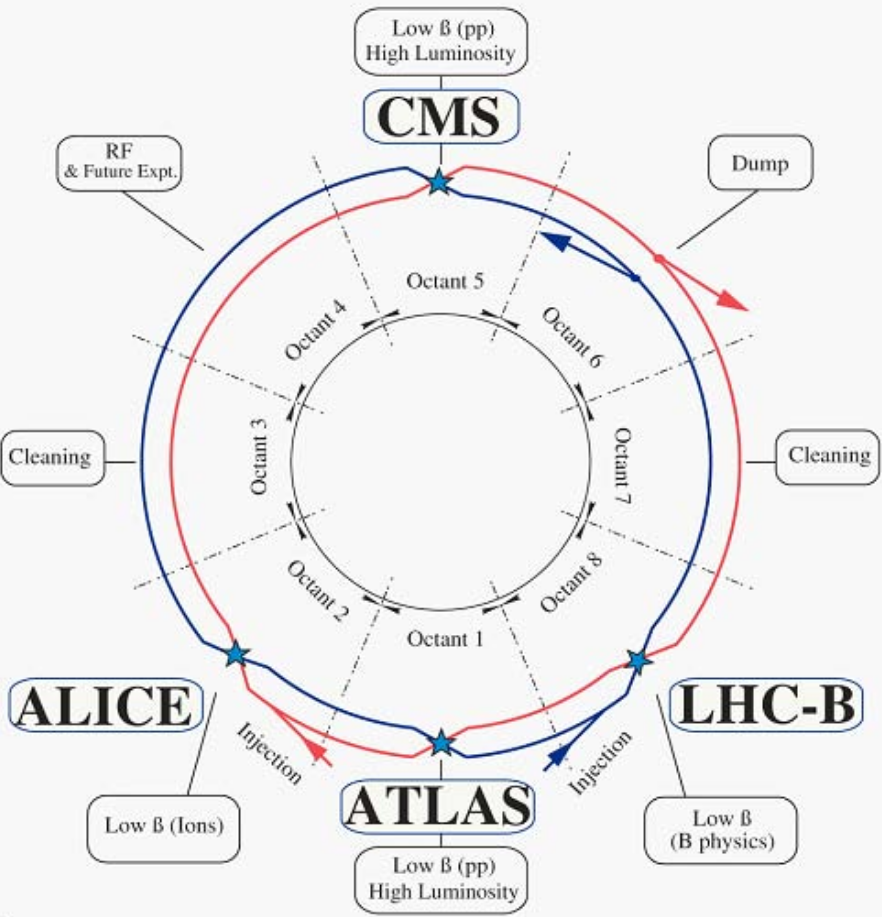
\includegraphics{Detector/Figures/LHC.png}}

\caption{Schematic of the LHC ring showing the two beams as well as the four major experiments. It also shows the injection points as well as the cleaning point and the beam dump. \cite{1748-0221-3-08-S08001}
  \label{fig:det_LHC}}
  \end{center}
\end{figure}

The instantaneous luminosity $\mathcal{L}$ is a measure for the rate of pp collisions.
It is related to the rate of events $\dot N$ of a process $k$ through the cross section $\sigma_k$:

\begin{equation}
\dot N_k = \mathcal{L} \cdot \sigma_k.
\end{equation}

The luminosity itself can be calculated from the beam properties:.

\begin{equation}
\mathcal{L} = \frac{N_b \cdot N_p^2 \cdot v}{\Sigma_x \Sigma_y}.
\end{equation}

Here, $N_b$ stands for the number of bunches, $N_p$ for the number of protons per bunch and $v$ for the rotation frequency of the LHC.
$\Sigma_x$ and $\Sigma_y$ are the effective widths of the overlap of the two beam profiles in x or y direction respectively. The luminosity is determined by measuring those beam profiles.
Special LHC conditions are used to calibrate the relevant parts of the detector for this measurement of the beam profiles. In a Van-der-Meer scan \cite{Zanetti:1357856} the two beams are shifted against each other, which allows to calibrate the detector for known configurations of $\Sigma_x,y$.
The calibrated detectors are then used to determine the instantaneous luminosity during data taking. 

In this analysis the data corresponds to an integrated luminosity of \lumivwunc taken at a center of mass energy of $\sqrt{s} = 13 \TeV$.

\section{The CMS detector}

The CMS experiments detector is a multi purpose detector for the study of particles from proton-proton, proton-lead and lead-lead collisions.
With a length of $21.6 \;\si{\meter}$ and a  diameter of $15 \;\si{\meter}$ it is relatively small and dense for its weight of 14000 tons \cite{Bayatian:922757}, thus the name 'compact'.

The detector is built of multiple radial layers ("onion structure") and split into a barrel region in the middle and two endcaps closing the detector structure as shown in the overview in Figure \ref{fig:det_CMS}.
The innermost part of the detector is the tracker, followed by the electromagnetic and then the hadronic calorimeter.
These parts of the detector are surrounded by the superconducting solenoid. The muon system is the last part of the detector and is situated outside the solenoid. It is interleaved with the iron return yoke of the magnet.

\begin{figure}[htbp!]
  \begin{center}
      \resizebox{0.89 \textwidth}{!}{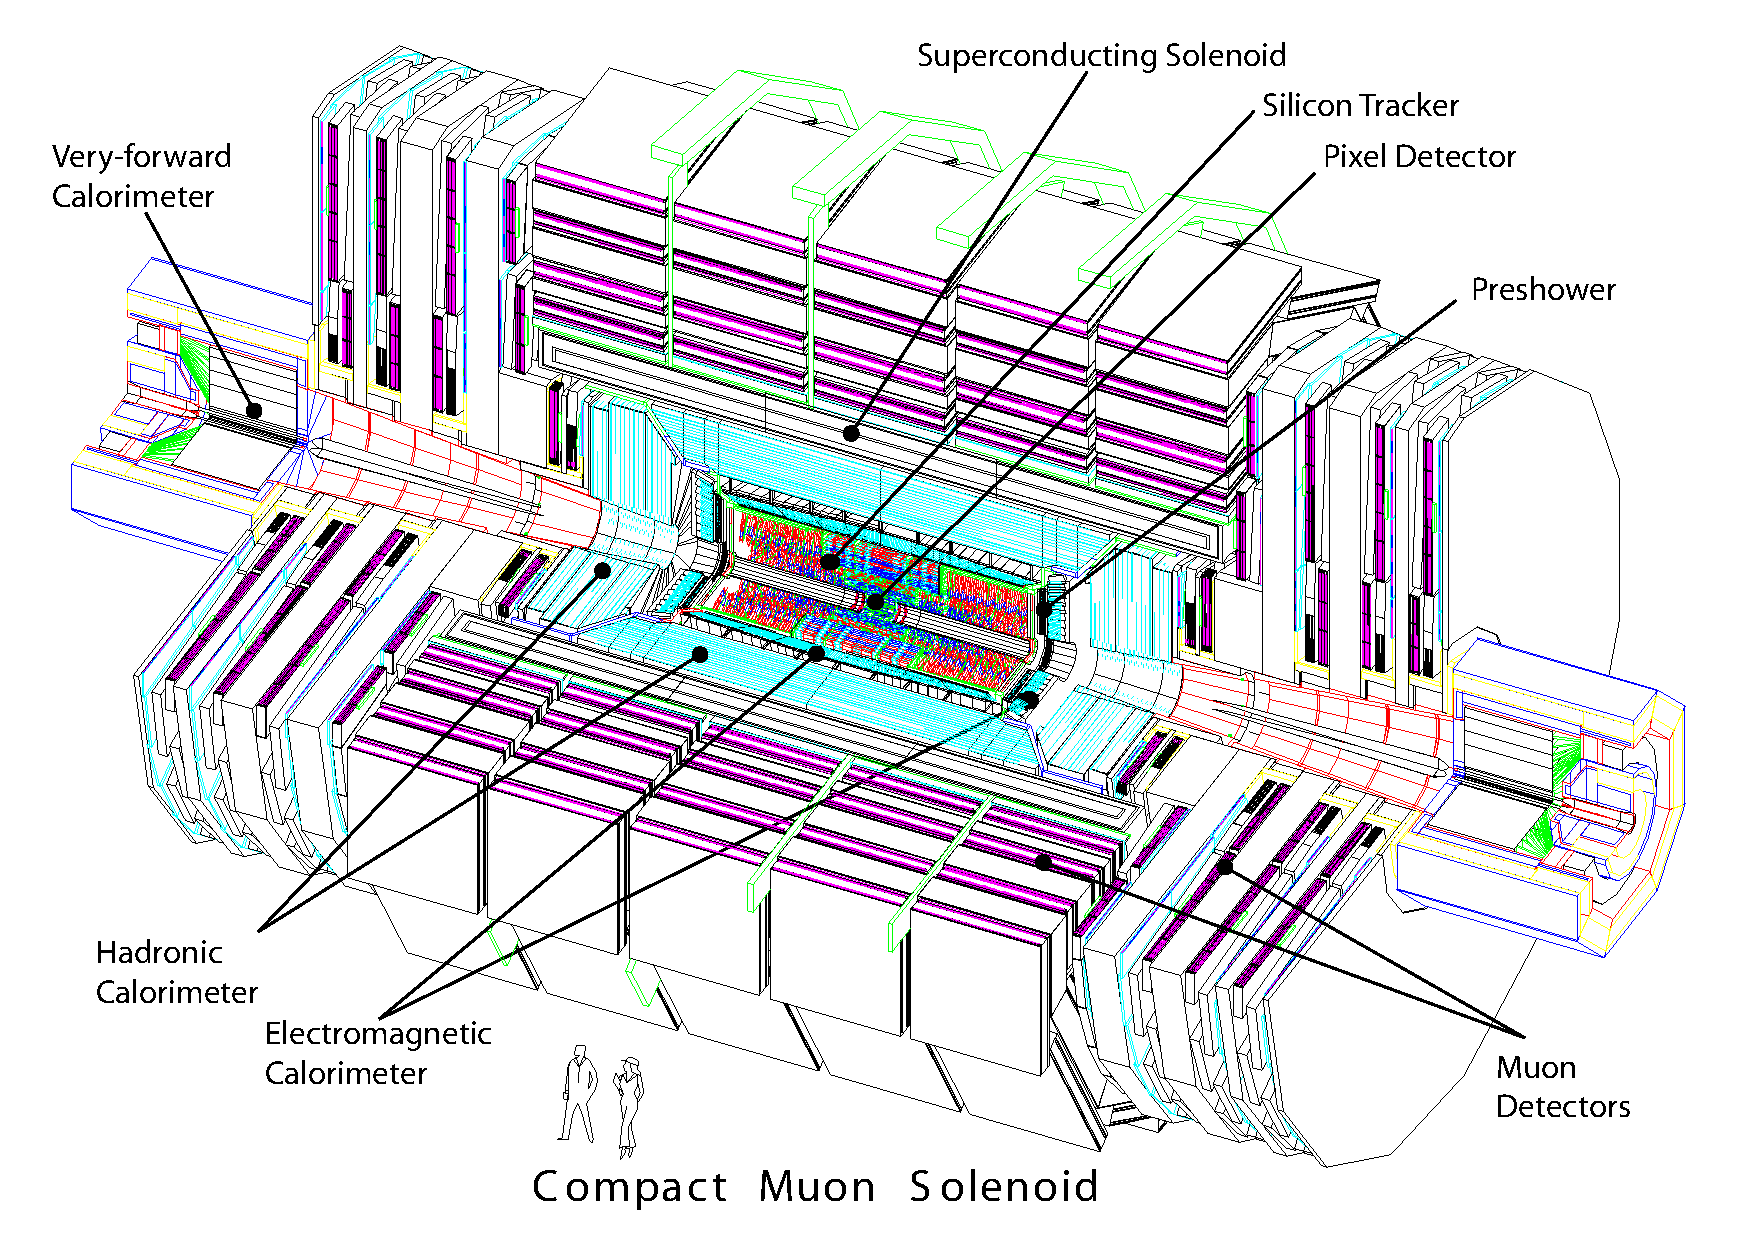
\includegraphics{Detector/Figures/cms_complete_labelled}}

\caption{The CMS detector and its relevant subsystems. \cite{Collaboration:1433717}
  \label{fig:det_CMS}}
  \end{center}
\end{figure}


The solenoid provides a magnetic field of $3.8 \;\si{\tesla}$ for the inner part of the detector (the tracker and calorimeters) and a field of about $2 \;\si{\tesla}$ in the muon system.
A total energy of $2.6 \;\si{\giga \joule}$ is stored in 2168 loops of superconducting cables.
This strong magnetic field leads to strongly bent tracks for charged particles, allowing a precise measurement of their momenta. 
The tracks of particles outside the magnet are bent in the opposite direction of those in the inner part.

The detector is described in a right-handed coordinate system with the origin in the interaction point.
The z-axis points in the direction of the counterclockwise beam, the y-axis points vertically upwards and the x-axis radially points towards the center of the LHC ring.
The $\varphi$ angle is defined in the x-y plane, while the angle $\theta$ is defined in the y-z plane. Instead of $\theta$ the pseudorapidity $\eta$ is used, since it is invariant under Lorentz transformation as long
as the momentum of a particle is large compared to its mass ($|\vec{\mathrm{p}}|\gg \mathrm{m}$):

\begin{equation}
\eta = -\ln{\tan{\frac{\theta}{2}}}.
\end{equation}

The subsequent sections describe the different parts of the detector including the triggering system that is used to select the collisions for which the data is stored for offline analysis.


\subsection{The tracking system}
\label{set:det_tracker}

The tracking system \cite{Bayatian:922757} is designed to measure both tracks and vertices with the highest possible precision.
This requires high granularity and, in the LHC environment, a fast response.

The tracking system is comprised of two parts: the inner one with pixels, the outer one with strips.
Its structure in the barrel as well as the endcaps is shown in Figure \ref{fig:det_Tracker}.

\begin{figure}[htbp!]
  \begin{center}
      \resizebox{0.75 \textwidth}{!}{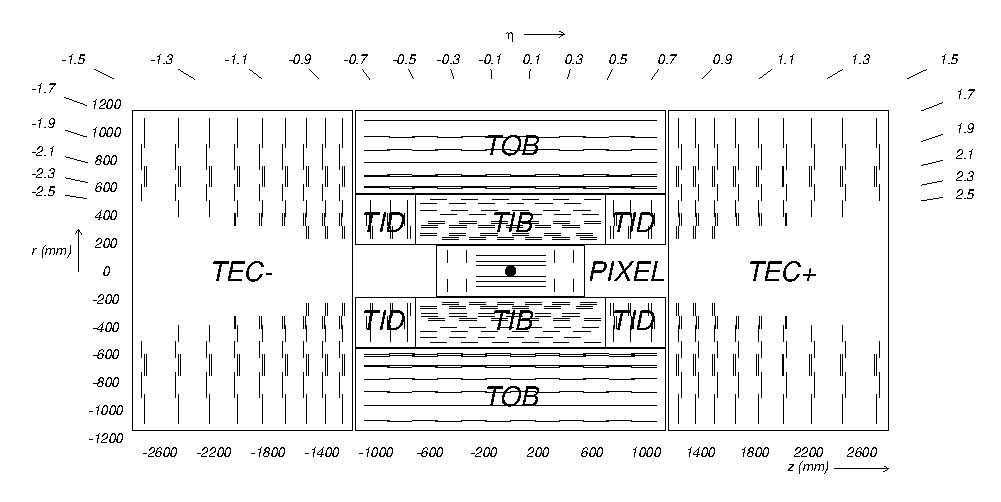
\includegraphics{Detector/Figures/TrackerLayout}}

\caption{The tracking system of the CMS detector in the barrel and endcap regions. The sketch shows the pixel as well as the strip tracker. The strip tracker consists of the inner barrel (TIB), outer barrel (TOB), inner disks (TID) and endcaps (TEC) parts \cite{Dominguez:1481838}.
  \label{fig:det_Tracker}}
  \end{center}
\end{figure}



The first pixel layer is located at a radius of $4.4 \;\si{\centi \meter}$ in the barrel and at $34.5 \;\si{\centi \meter}$ in the endcaps.
Both parts cover a range of $|\eta| < 2.5$.
The barrel region includes three layers of pixel detectors and ten layers of strip detectors, while the endcap includes two layers of pixels and twelve layers of strips.
The 66 million pixels measure $150 \times 100 \; \si{\micro \meter}$. The 9.6 million strips have a width of $80-180  \;\si{\micro \meter}$, together with the pixel that allows to separate even closely spaced
particle trajectories.
The position of each tracker part is precisely known from alignment analyses using tracks from collision events and cosmic muons \cite{Chatrchyan:2014wfa}.

The momenta of charged hadrons with a $\pt < 20 \GeV$ are measured with a resolution of $1\%$ at an incidence of ninety degrees \cite{Sirunyan:2017ulk}. The relative resolution decreases for higher \pt, reaching a resolution corresponding to 
the energy resolution of the calorimeter at several hundred \GeV. 
At low \pt, the resolution is dominated by multiple scattering of the particle in the tracker material \cite{1748-0221-9-10-P10009}. At high \pt, the resolution decreases as the bent of the track is
reduced making the \pt determination more difficult. The resolution in \pt is shown in Figure \ref{fig:det_trackeffs} for muons and charged pions.
Since high \pt partons usually produce multiple charged hadrons of lower \pt through fragmentation, the tracker can still contribute significantly 
to the measurement of high \pt jets.

\begin{figure}[htbp!]
  \begin{center}
      \resizebox{0.49 \textwidth}{!}{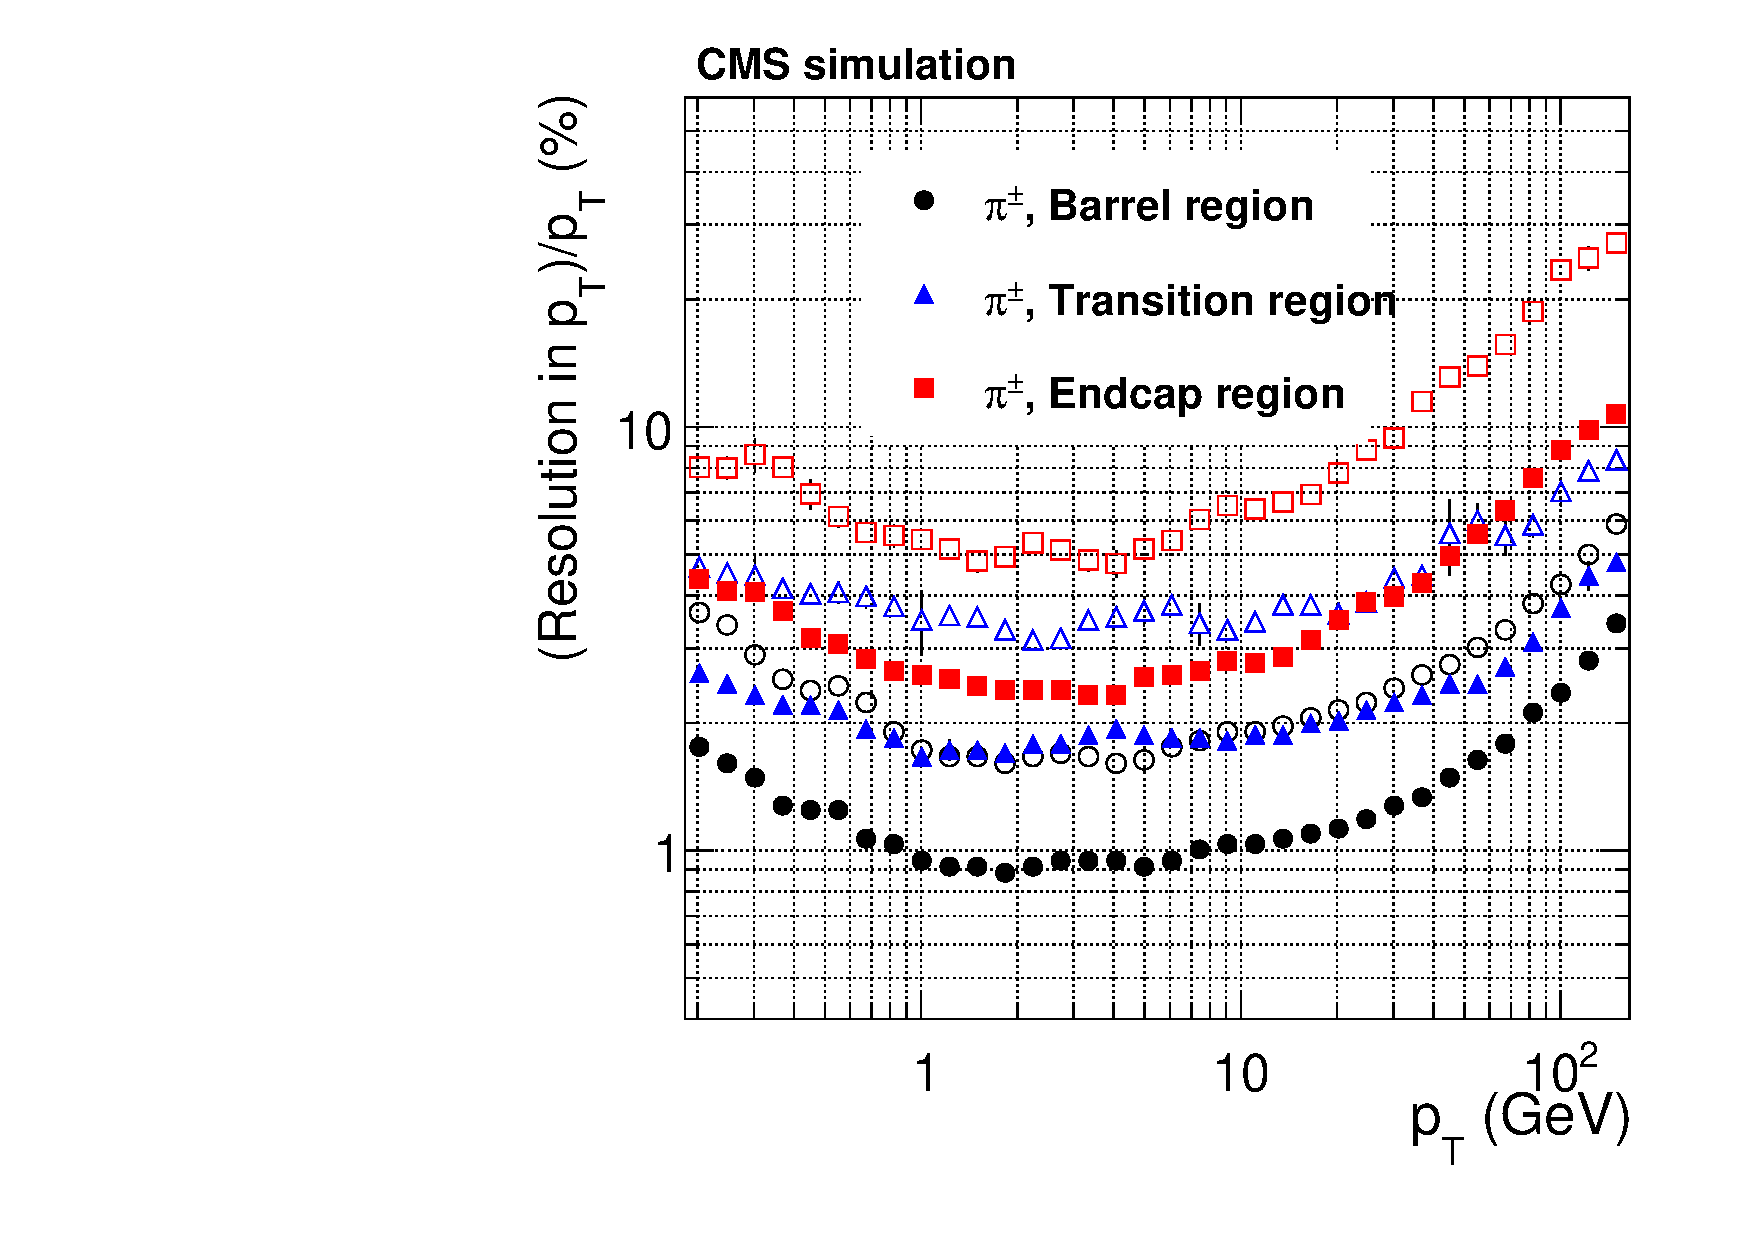
\includegraphics{Detector/Figures/trackpipt}}
      \resizebox{0.49 \textwidth}{!}{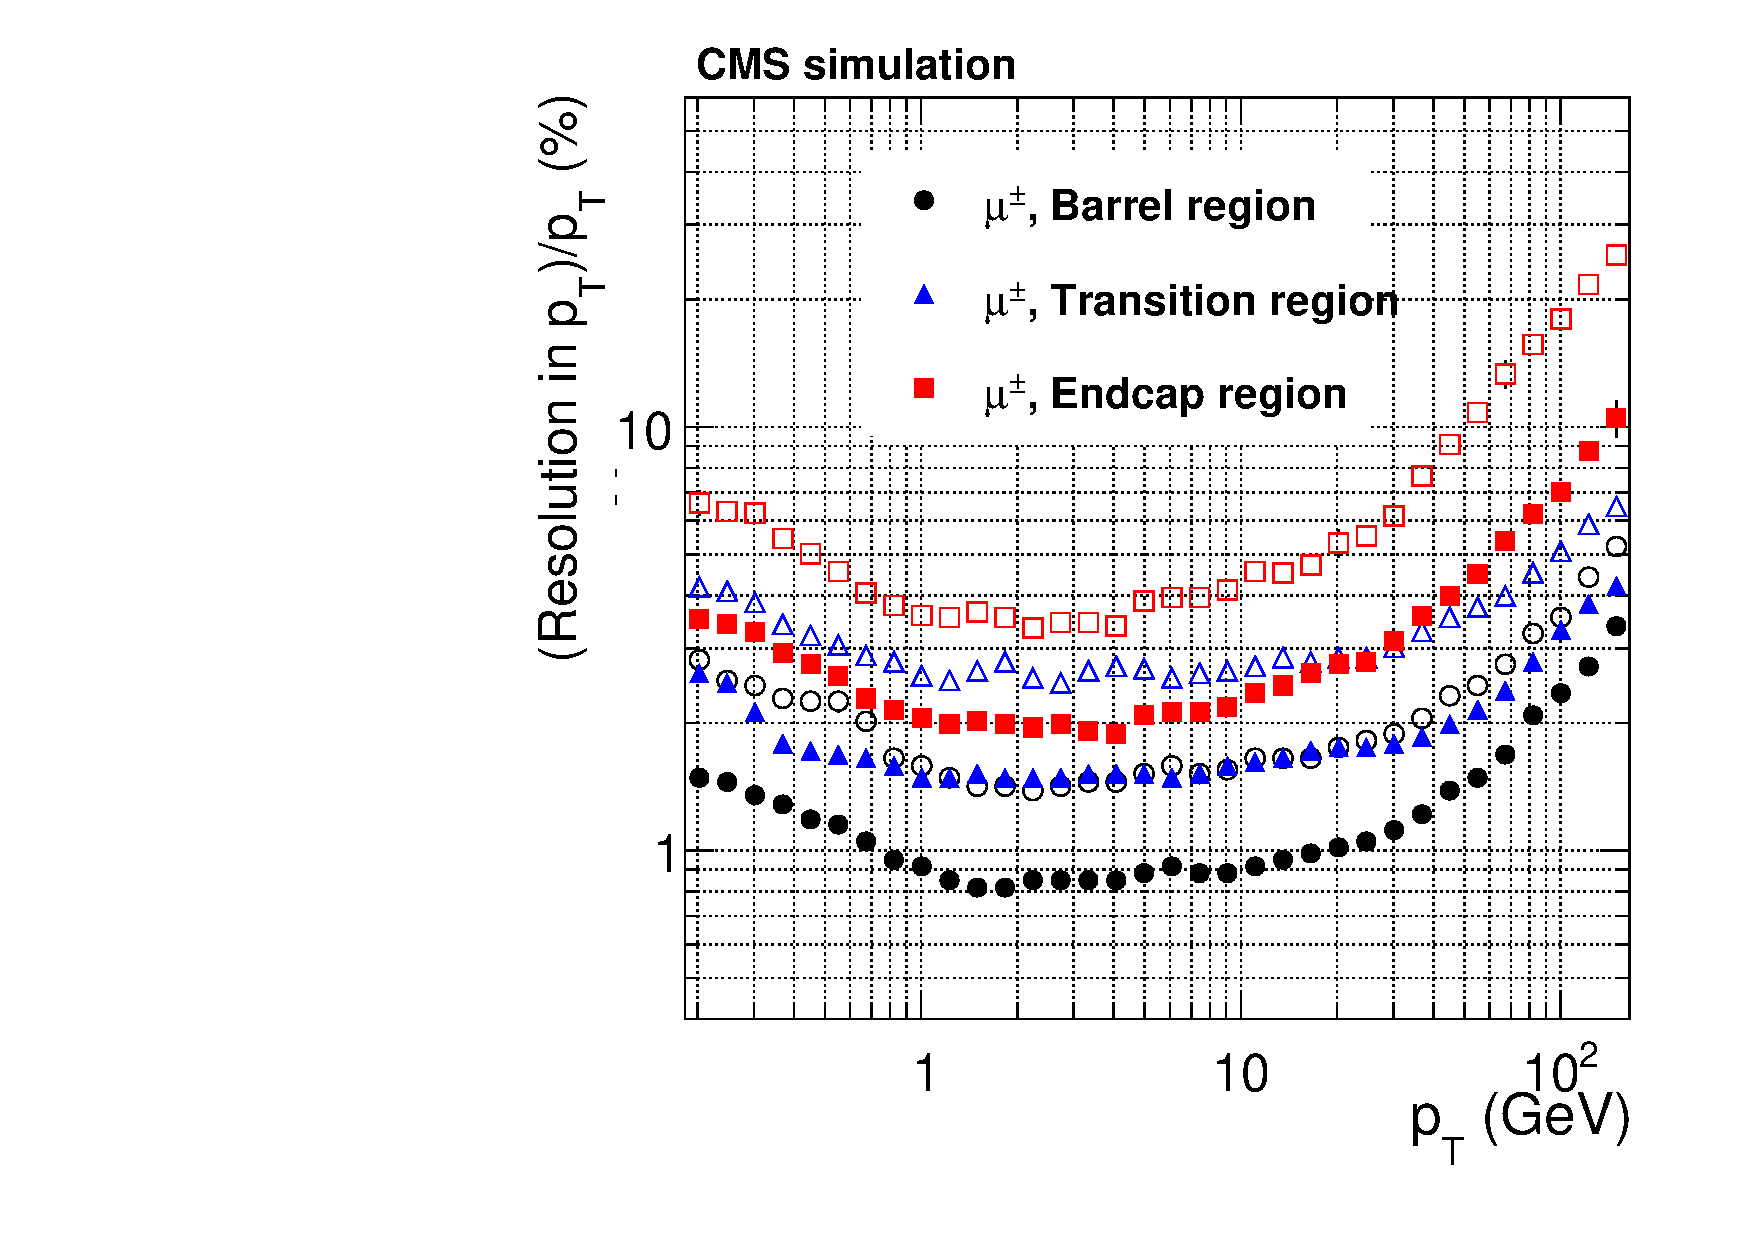
\includegraphics{Detector/Figures/trackmupt}}

\caption{Track \pt resolution depending on the track \pt for simulated charged pions (left) and muons (right). \cite{1748-0221-9-10-P10009}.
  \label{fig:det_trackeffs}}
  \end{center}
\end{figure}


\subsection{The electromagnetic calorimeter}

The electromagnetic calorimeter (ECAL)\cite{Bayatian:922757} measures the energy of electrons and photons that produce showers in the ECAL.
These electromagnetic showers should be contained within the ECAL. Additionally, the high granularity of the ECAL helps separate the signals from different particles.
A sketch of the structure of the ECAL is shown in Figure \ref{fig:det_ECAL}.

\begin{figure}[htbp!]
  \begin{center}
      \resizebox{0.75 \textwidth}{!}{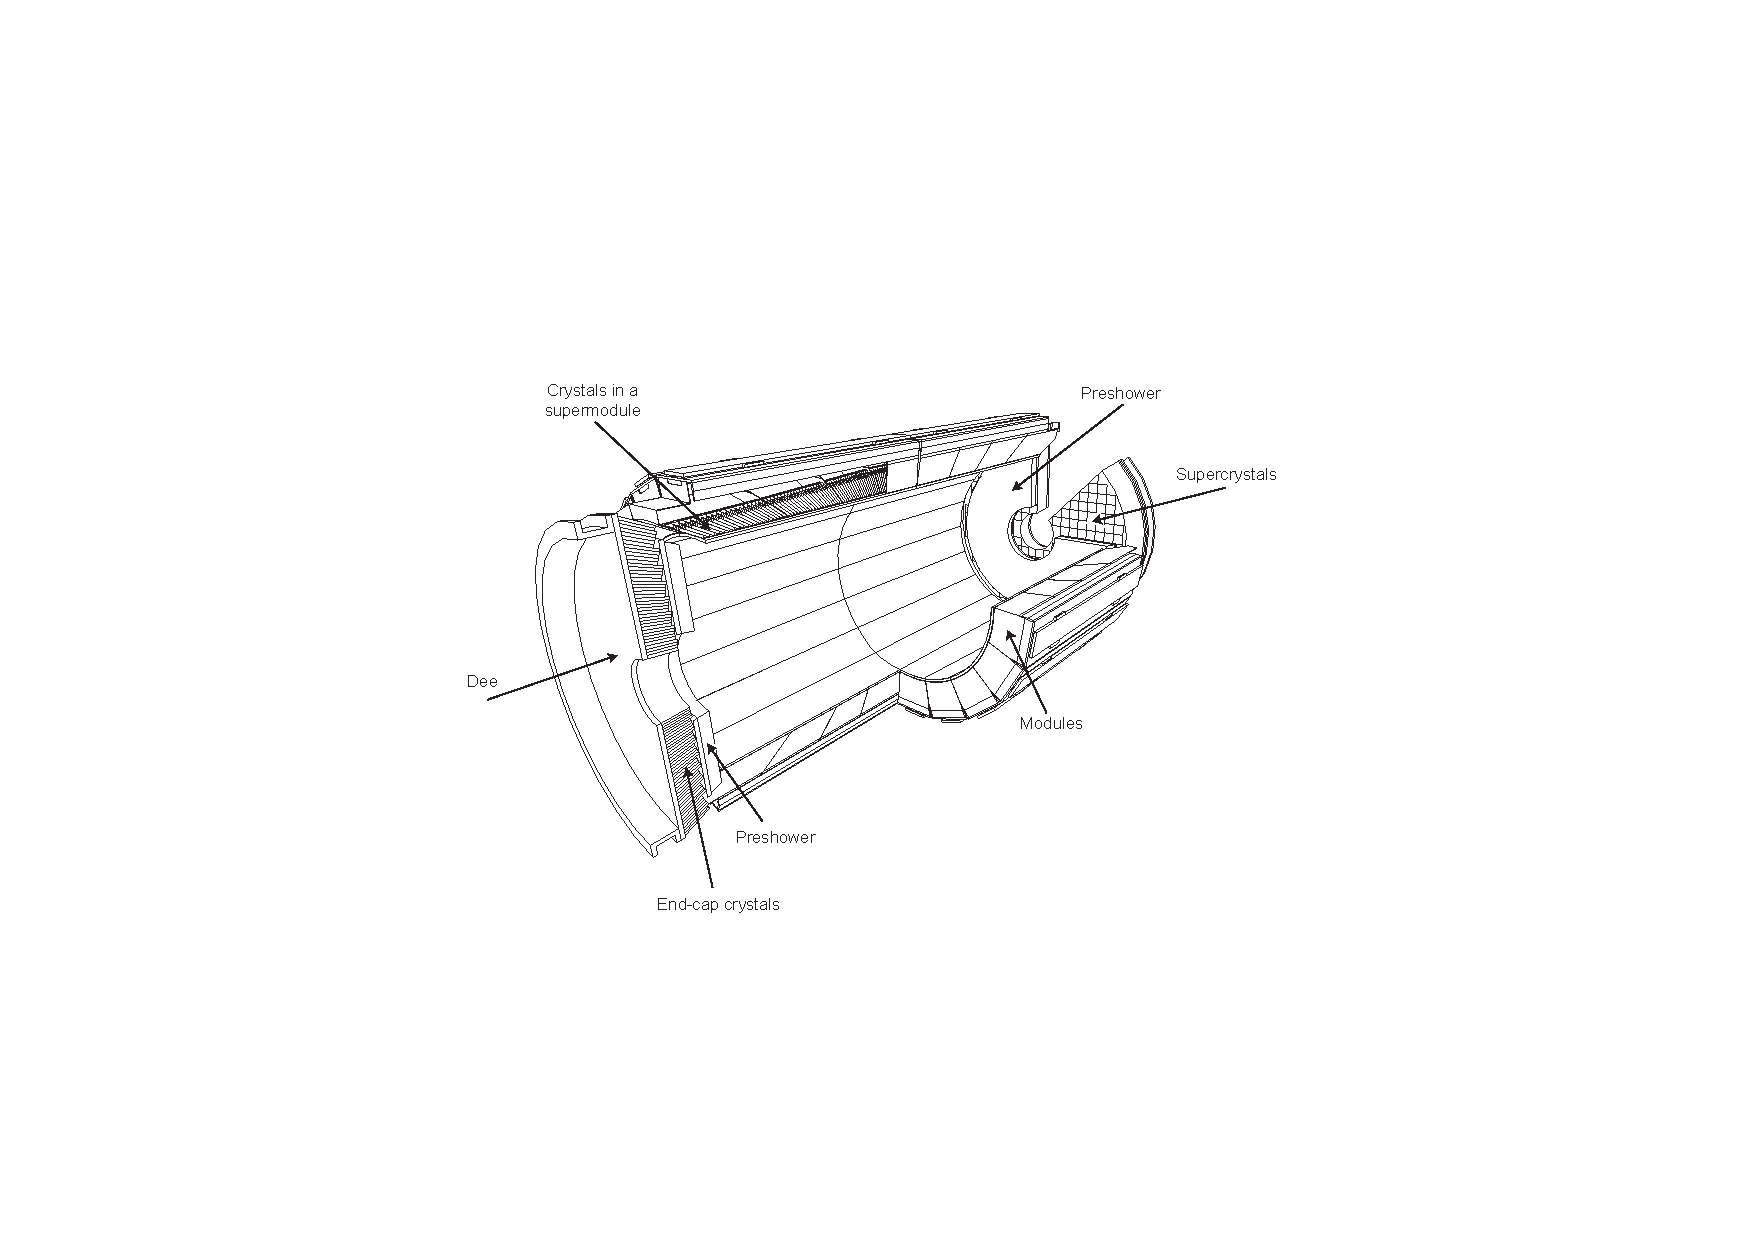
\includegraphics{Detector/Figures/ECAL}}

\caption{A sketch of the electromagnetic calorimeter showing the structure in the barrel and the endcaps as well as the preshower detectors. \cite{Chatrchyan:2009qm}.
  \label{fig:det_ECAL}}
  \end{center}
\end{figure}

The ECAL is made of lead tungstate with the barrel region covering about $|\eta| < 1.5$ and the endcaps covering $1.5 < |\eta|<3.0$. The crystals are $23 (22)  \;\si{\centi \meter}$ in the barrel (endcap) corresponding to about 26(25) radiation lengths.
For electrons and photons up to an energy of $1 \TeV$, more than $98  \%$ of the energy of each particle is completely contained in the ECAL.
The crystal depth also corresponds to roughly one interaction length. This implies that approximately two thirds of the hadrons start their shower in the ECAL.

The front of the crystals has a size of $2.2 \times 2.2 \;\si{\centi \meter \squared}$ in the barrel and $2.2 \times 2.2 \;\si{\centi \meter \squared}$ in the endcaps. This size corresponds to the Moliere radius of the 
lead tungstate of $2.2 \;\si{\centi \meter}$.
The electronic noise in the ECAL is measured to be about $40 \MeV$ per crystal in the barrel and about $100 \MeV$ in the endcaps.

The energy resolution for an electron measured in the ECAL can be parameterized depending on the electron energy as follows \cite{Sirunyan:2017ulk}:

\begin{equation}
\frac{\sigma}{\mathrm{E}} = \frac{2.8\%}{\sqrt{\mathrm{E}/\GeV}} \oplus \frac{12\%}{\mathrm{E} / \GeV} \oplus 0.3\%.
\end{equation}

The first term represents a stochastic term caused by fluctuations such as the amount of intrinsic variations of the showering itself. The second term is caused by noise from the electronics and the constant third term is related
to calibration uncertainties, detector non-uniformity and radiation damage.

Photons in jets have a typical energy range of $1-50 \GeV$ where the resolution of the ECAL is excellent.

The so-called preshower detector is situated in front of the two ECAL disks in the endcaps.
The preshower contains two layers: The first is a lead radiator followed by silicon strip sensors.
The detector has a much higher granularity than the ECAL, which allows measuring the initial position of a shower from an electron or photon with a high precision.
The purpose of the preshower is to discriminate  between neutral pions decaying into two photons and prompt single photons.
Additionally, a coincidence between ECAL and preshower can be used to identify electrons and photons.
The performance of the preshower is degraded through a large number of neutral pions resulting from hadrons interacting with the tracker material.

\subsection{The hadronic calorimeter}

The hadronic calorimeter (HCAL)\cite{Bayatian:922757} is a sampling calorimeter consisting of layers of brass absorbers and plastic scintillators.
Its purpose is to measure the energy of hadronic showers with a high precision. Additionally, it prevents the hadronic showers from leaking into the muon system.
In the barrel it covers a range of $|\eta|< 1.3$ with a corresponding endcap coverage of $1.3 <|\eta|< 3.0$.
In the barrel it is about six interaction lengths thick at normal incidence, increasing to over ten interaction lengths at lower incidence angles.
The whole HCAL is shown as a sketch in Figure \ref{fig:det_HCAL}.



\begin{figure}[htbp!]
  \begin{center}
      \resizebox{0.75 \textwidth}{!}{\includegraphics{Detector/Figures/hcaldisplay.eps}}

\caption{A quarterly schematic of the hadronic calorimeter showing the HCAL in the barrel(HB) and the endcaps(HE), the outer HCAL (HO) and the forward HCAL (HF)  \cite{2010JInst...5T3014C}.
  \label{fig:det_HCAL}}
  \end{center}
\end{figure}



The outer hadronic calorimeter (HO) is situated outside the solenoid coil, increasing the interaction length as an additional absorber.
In the very central region, the interaction length is further increased by additional layers of steel.
Including the ECAL, the total calorimeter system has a thickness corresponding to a minimum of about twelve interaction lengths in the barrel and ten interaction lengths in the endcaps.
The individual towers of the ECAL have a cross section of $\Delta \eta \times \Delta \varphi = 0.087 \times 0.087$ in the central region of $|\eta|< 1.6$ and a cross section of $\Delta \eta \times \Delta \varphi = 0.017 \times 0.017$
in the more forward region \cite{Bayatian:922757}.

The electronic noise is measured to be about $200 \MeV$ per tower \cite{Sirunyan:2017ulk}.
The combined energy resolution for ECAL and HCAL has been measured with a pion beam to be 

\begin{equation}
\frac{\sigma}{\mathrm{E}} = \frac{110\%}{\sqrt{\mathrm{E}/\GeV}} \oplus 9\%.
\end{equation}

The two parts of the hadron forward calorimeter (HF) are positioned in the very forward(backward) region of the detector at a distance of $11 \; \si{\meter}$ from the interaction point.
It covers a region of up to $|\eta| \approx 5$. It consists of steel absorbers and quartz fibers of two different lengths. The long quartz fibers correspond to roughly ten interaction lengths. The difference in the signal from the short and the long fibers is used to estimate the hadronic and electromagnetic components of the shower.

\subsection{The muon system}

High energy muons mostly interact with matter through ionization.
They are generally neither stopped by nor decay within the detector, so the momentum can only be measured by reconstructing their tracks.

The purpose of the muon system as the outermost part of the detector is to identify muons and measure their momentum.

The muon system \cite{Bayatian:922757} consists of four layers with three steel layers of the return yoke of the solenoid between them.
The central region is covered by Drift Tubes (DT) in the region of $|\eta|< 1.2$. The outer region is covered by Cathode Strip Chambers (CSC) in the region of $0.9<|\eta|<2.4$.
Additionally, Resistive Plate Chambers (RPC) cover the range of $|\eta|<1.6$.
A sketch of the whole muon system is shown in Figure \ref{fig:det_muon}.

\begin{figure}[htbp!]
  \begin{center}
      \resizebox{0.75 \textwidth}{!}{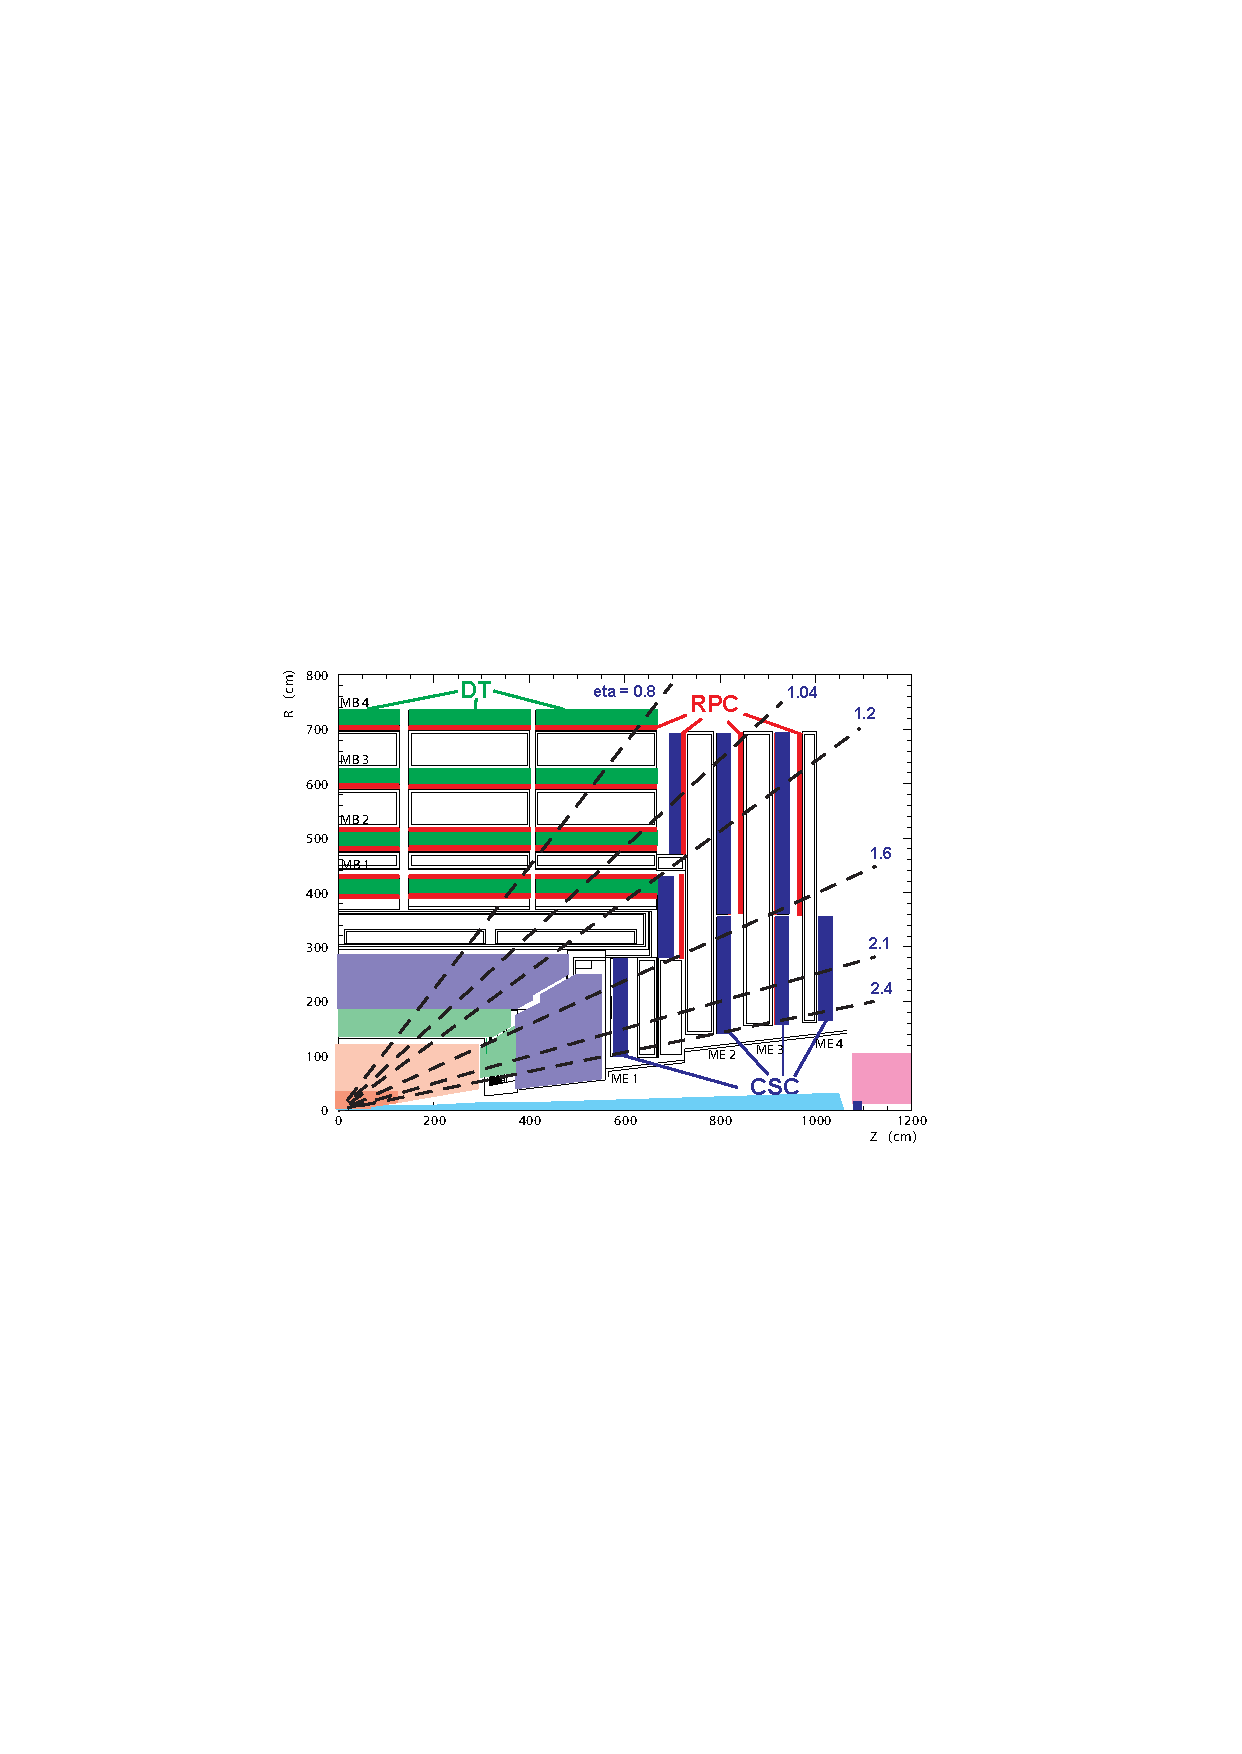
\includegraphics{Detector/Figures/Muon}}

\caption{A quarterly schematic of the muon system showing the Drift Tubes(DT) in the central part, the Cathode Strip Chambers(CSC) in the outer part and the Resistive Plate Chambers(RPC). \cite{Bayatian:922757}.
  \label{fig:det_muon}}
  \end{center}
\end{figure}

The DT chambers are filled with a mixture of argon and carbon dioxide. The chambers themselves contain layers which are rotated against each other,
which allows measuring both the $\varphi$ and the $\eta$ projection of the track. The DTs are also used for triggering.

The CSCs are positioned at a right angle with respect to the DTs. The single chambers consist of six gas gaps each. The two coordinates of the track are determined by radial cathode strips and perpendicular anode wires.
The spatial resolution of both the CSCs and the DTs is in the range of $100-200 \; \si{\micro \meter}$, depending on $\eta$.

The RPC system consists of 480 chambers. Their very high time resolution in the sub nano second range allows them to be used for triggering and the association of single muon tracks with a specific bunch crossing.

\subsection{Triggering}
\label{set:det_trigger}

The LHC delivers a collision rate of $40 \;\si{\mega \hertz}$. In order to record the data as it is measured by the detector, this data volume has to be reduced to a manageable size by
only keeping those events for further study in which a relevant result is observed. A two-tiered triggering system is used to reduce the final rate of events to $100 \;\si{\hertz}$.
First the hardware-based Level-1 (L1) Trigger is used to reduce the number of events for the software-based high-level trigger (HLT) \cite{Bayatyan:706847,Tapper:2013yva}.

The L1 trigger consists of programmable electronics using information from the calorimeters as well as the muon system as shown in Figure \ref{fig:det_Trigger}. The L1 trigger is separated into the muon trigger and the calorimeter trigger. The tracking system is not used at this stage of triggering.
 The muon trigger combines track information from the CSCs, DTs and RPCs. It uses information from the calorimeters for the isolation of the muons.
The calorimeter trigger combines the ECAL, HCAL and HF. Besides muon triggers, algorithms targeting electrons/photons, taus, jets and the overall energy deposition in the detector are used. Requiring a muon to be contained within a jet allows to target jets originating from a b quark where the B-hadron decays further into a final state containing a muon.
The L1 trigger has a maximal latency of $3.8  \;\si{\micro \second}$ in which a trigger decision has to be delivered to the HLT.

\begin{figure}[htbp!]
  \begin{center}
      \resizebox{0.75 \textwidth}{!}{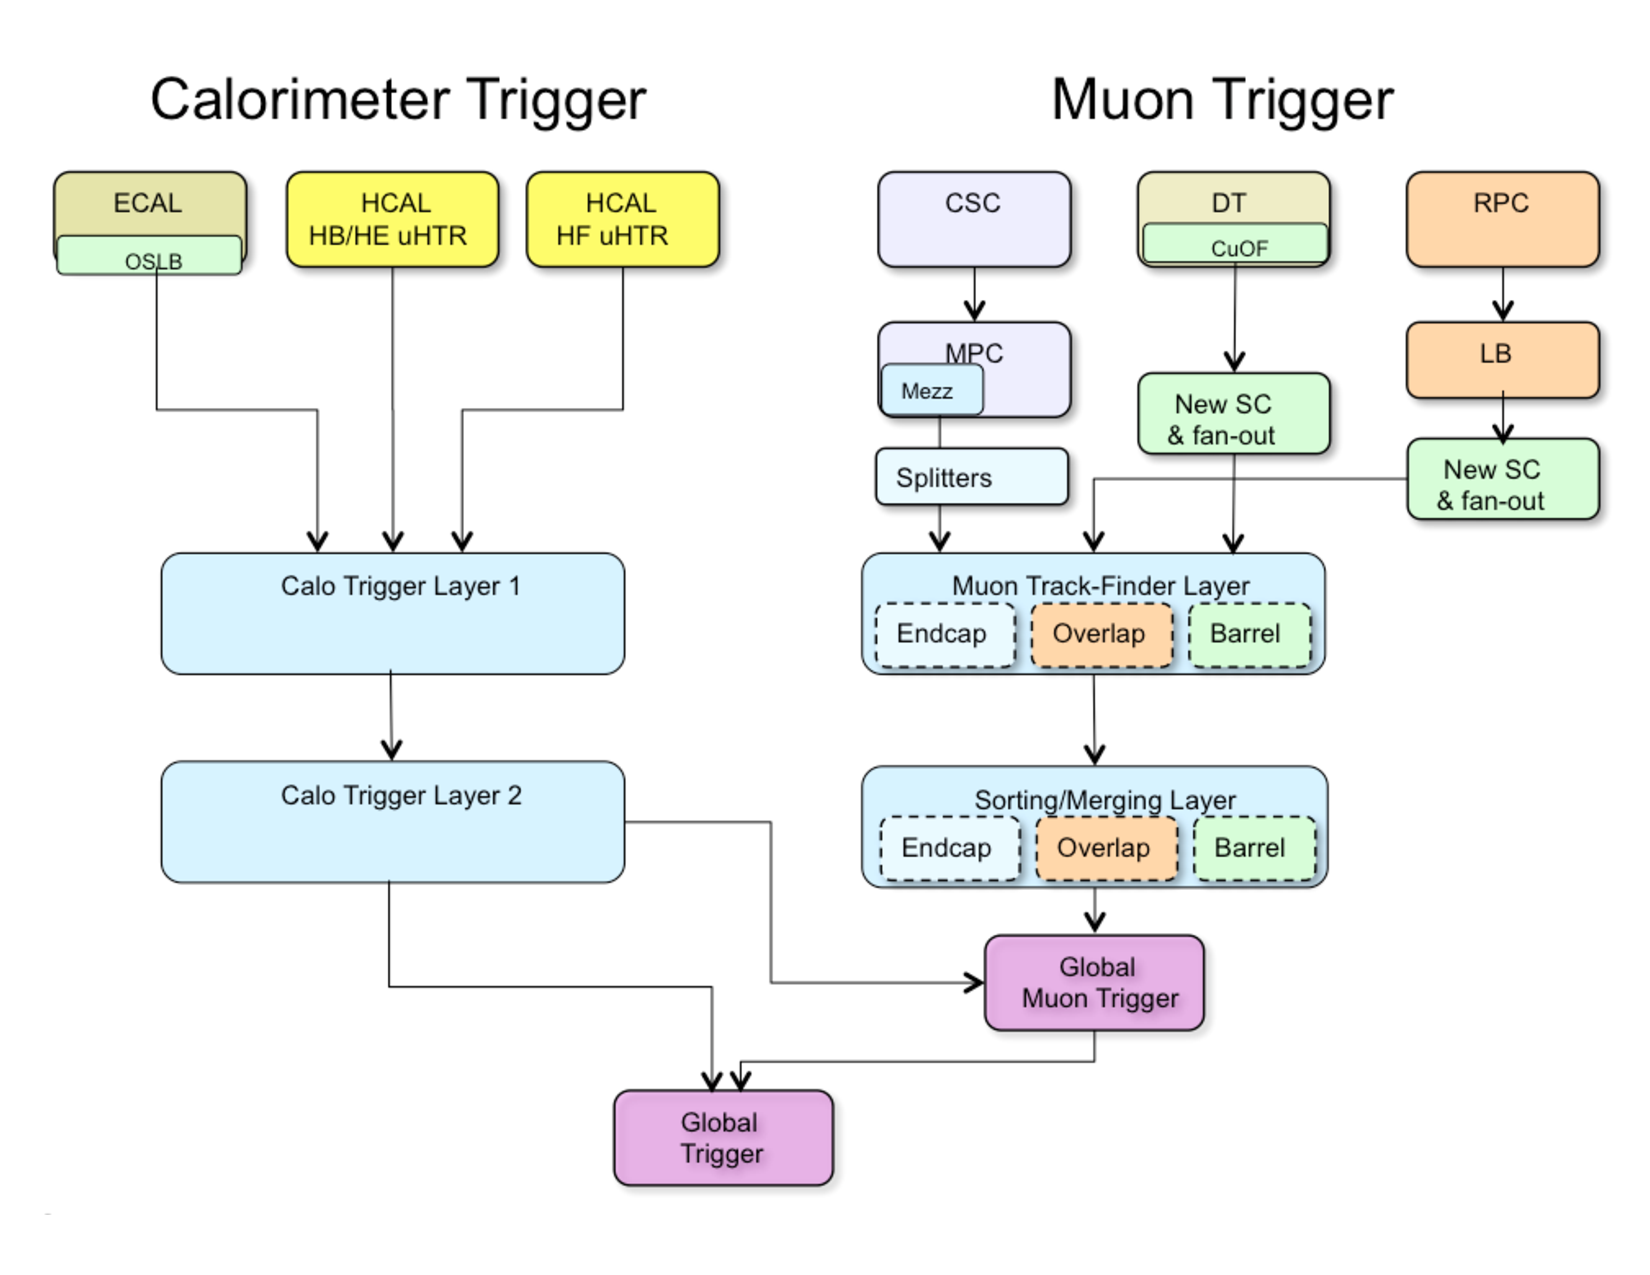
\includegraphics{Detector/Figures/Trigger}}

\caption{ Dataflow of the L1 trigger system showing the combination of information from the different subsystems \cite{Tapper:2013yva}.
  \label{fig:det_Trigger}}
  \end{center}
\end{figure}

The HLT is the second step of the triggering system. It reduces the number of events from $100 \; \si{\kilo \hertz}$ to $100 \; \si{\hertz}$.
Compared to the L1 trigger, it uses more sophisticated reconstruction techniques, which are generally close to the final reconstruction that is used for analysis.
The HLT starts from the L1 decision. It then combines information from the complete detector, including tracks, to reconstruct the respective particle in the path.
Finally, further thresholds on the kinematics, the isolation or the reconstruction quality are required. 
These steps are performed sequentially. If one step fails the sequence is stopped. 

In order to be able to reduce the rate of certain trigger paths for both the L1 and the HLT, some trigger paths only consider a fraction of events. This technique is called prescaling. If a trigger path is prescaled by two it only considers every second event.

A detailed study of the lepton triggers which are used in this analysis is presented in Chapter \ref{sec:Trigger}. The measurement of the trigger efficiency is 
discussed as well.


%!TEX root = ../thesis.tex
%*******************************************************************************
%****************************** Second Chapter *********************************
%*******************************************************************************

\chapter{Simulation and Reconstruction}

\section{Simulation}

\section{Reconstruction}

\subsection{The Particle Flow Algorithm}

\subsection{Electron Reconstruction}

\subsection{Muon Reconstruction}

\subsection{Identification of b-Jets}


%!TEX root = ../thesis.tex
%*******************************************************************************
%*********************************** First Chapter *****************************
%*******************************************************************************

\chapter{Trigger Efficiency measurement}  %Title of the First Chapter

The uncertainty on the trigger efficiency determination has been one of the dominant systematic uncertainties in \sttbar measurements.
Consequently, measuring the trigger efficiency with the highest possible precision is an important part of improving the precision of these
measurements. In the measurement the simulation is rescaled according to the difference between the trigger efficiency in data and simulation. 
So the trigger efficiency needs to be measured independently in both data and simulation.

This chapter describes the trigger selection used in this measurement and how this selection can already help to improve
the later efficiency measurement (see Section \ref{sec:TriggerSel}). It is further explained how the efficiency of this trigger selection is measured(see Section \ref{sec:TriggerMetMethod}). In order to estimate the precision of this measurement the trigger efficiency
is also measured with another method (see Section \ref{sec:TriggerTPMethod}). The two results are finally compared (see Section \ref{sec:TriggerComp}) and the chapter concludes with the final scale factor between data and simulation (see Section \ref{sec:TrigSF}). 



%********************************** %First Section  **************************************
\section{Trigger Selection} %Section - 1.1 
\label{sec:TriggerSel}

The trigger selection is optimized for maximum efficiency. This allows to use a high amount of data in the measurement and reduces the uncertainty on the trigger efficieny. as a higher efficiency leads to a lower statistical uncertainty due to the statistical properties of the binomial distribution.
The efficiency itself is measured with respect to the reconstruced (also called offline) objects (see Section XX for details
on this reconstruction).

For a di-lepton selection the starting point are of course the di-lepton triggers. There are different triggers depending on the flavor of each of the
two leptons. These triggers typically have assymetric cuts on the \pt of the two leptons, so the leading lepton has a significantly higher pt requirement than
the trailing lepton. In general the quantities reconstructed for the trigger are slightly different from the objects used in the offline analysis. This
leads to an in-efficiency of the trigger compared to the offline selection close to the kinematic requirements for the trigger objects.

In the case of the di-lepton trigger this mainly effects the efficiency at the cut-offs in \pt for the two leptons. One way to mitigate this is to
require a higher offline \pt for the leptons than is required by the trigger \todo{Ref to selection}.
Another way to reduce this inefficiency is to combine the di-lepton trigger with other triggers which only depend on one lepton, mitigating any
influence of the second lepton. This leads to a combination of di-lepton and single lepton triggers with a logical 'OR' in the trigger selection.
In general only unprescaled triggers are used in this analysis.

This combination increases the trigger efficiency by $\sim 10 \; \%$ compared to onyl using the di-lepton trigger.
This is shown in Figure \ref{fig:TriggerSel} for a dataset taken in 2016 in Run B to F.

\begin{figure}[htbp!]
  \begin{center}
    \resizebox{0.48 \textwidth}{!}{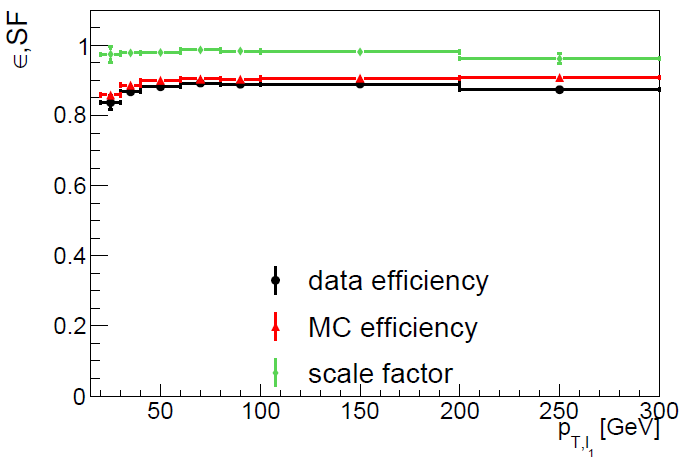
\includegraphics{Trigger/Figures/Trigger_pt_nosilep.png}}
    \resizebox{0.48 \textwidth}{!}{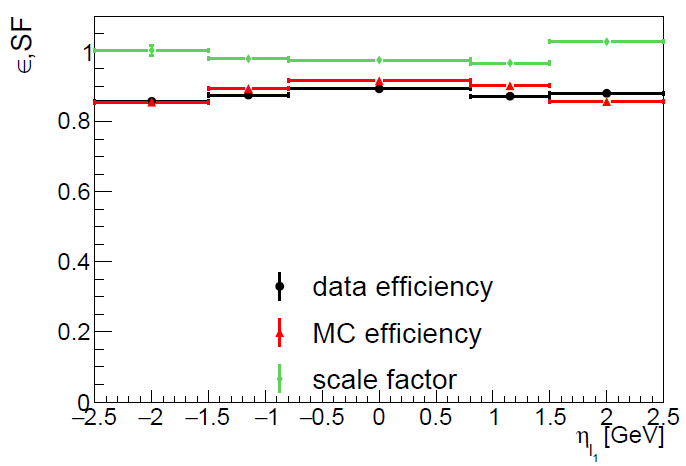
\includegraphics{Trigger/Figures/Trigger_eta_nosilep.png}}
    \resizebox{0.48 \textwidth}{!}{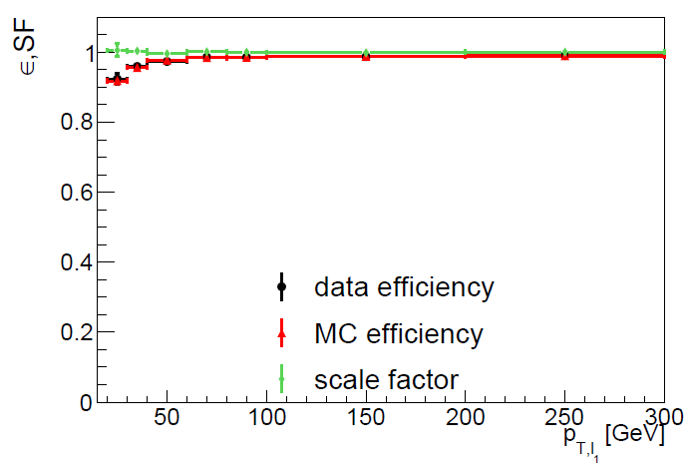
\includegraphics{Trigger/Figures/Trigger_pt.png}}
    \resizebox{0.48 \textwidth}{!}{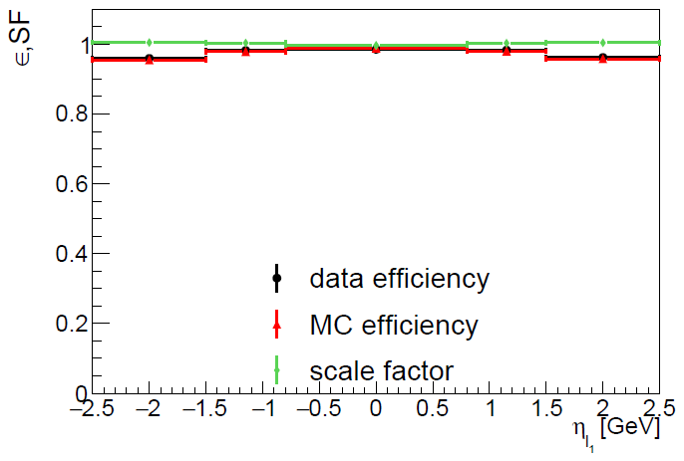
\includegraphics{Trigger/Figures/Trigger_eta.png}}
      \caption{Efficiencies of the trigger selection in the \emu channel for simulation and data and the corresponding scale factor. The top row shows the efficiency when using dilepton triggers only, while the bottom row shows
      the efficiency for a combination of dilepton and single lepton triggers. The left row shows the efficiency depending on the \pt of the leading lepton. The right column shows the efficiency depending on the $\eta$ of the leading lepton. }  
       \label{fig:TriggerSel}
  \end{center}
\end{figure}


The final trigger selection is a bit more complicated because we use unprescaled triggers with the most relaxed requirements possible.
This results in the trigger selection shown in Table \ref{tab:triggerSel} for each of the three di-lepton channels.
Double counting events is prevented by explicitly requiring triggers on their respective dataset, but vetoing them on the other datasets.

 \begin{table}[hbt]
    \centering
    \caption{The trigger selection that is applied on data. It can differ between the different run periods because of changing prescales.}
    \label{tab:triggerSel}
     \begin{tabular}
            {c|c|c}
            channel & run & trigger \\
            \hline
             \mumu & B-G & HLT\_Mu17\_TrkIsoVVL\_Mu8\_TrkIsoVVL \\
              & B-G & HLT\_Mu17\_TrkIsoVVL\_TkMu8\_TrkIsoVVL \\
              & H & HLT\_Mu17\_TrkIsoVVL\_Mu8\_TrkIsoVVL\_DZ \\
              & H & HLT\_Mu17\_TrkIsoVVL\_TkMu8\_TrkIsoVVL\_DZ \\
              & B-H & HLT\_IsoMu24 \\
              & B-H & HLT\_IsoTkMu24 \\
            \hline
             \ee &  B-H & HLT\_Ele23\_Ele12\_CaloIdL\_TrackIdL\_IsoVL\_DZ \\
              &  B-H & HLT\_Ele27\_WPTight\_Gsf \\
            \hline
             \empm & B-G & HLT\_Mu23\_TrkIsoVVL\_Ele12\_CaloIdL\_TrackIdL\_IsoVL \\
              & B-G & HLT\_Mu8\_TrkIsoVVL\_Ele23\_CaloIdL\_TrackIdL\_IsoVL \\
              & H & HLT\_Mu23\_TrkIsoVVL\_Ele12\_CaloIdL\_TrackIdL\_IsoVL\_DZ \\
              & H & HLT\_Mu8\_TrkIsoVVL\_Ele23\_CaloIdL\_TrackIdL\_IsoVL\_DZ \\
              & B-H & HLT\_Ele27\_WPTight\_Gsf \\
              & B-H & HLT\_IsoMu24 \\
              & B-H & HLT\_IsoTkMu24 \\
    \end{tabular}
\end{table}







%********************************** %Second Section  *************************************
\section{Method: Independent Triggers} %Section - 1.2
\label{sec:TriggerMetMethod}

In this analysis the trigger efficiency is mainly measured using a dataset taken with an orthogonal trigger selection.
In general this allows to measure the trigger efficiency without bias with the same method in data and simulation independently 
of each other. It is important that these independent triggers are indeed as independent from the dilepton triggers as possible
and for simplicity they should also be unprescaled in the full run range.  This allows to measure the trigger efficiency in the same
way in both data and simulation.

Here triggers based on missing transverse energy (\ETm) are used. They are especially usefull for a \ttbar analysis, 
as dileptonic \ttbar events should produce \ETm due to the two neutrinos. This allows to measure the trigger efficiency for data
in an event sample which at least contains \ttbar events. The efficiency in simulation can be measured on a sample of \ttbar events.
The correlation between the \ETm and dilepton triggers is studied in simulation and found to be minimal.

The trigger efficiency is then measured according to the formula given in Equation \ref{eq:TriggerEff}, where $N$ denotes the number of 
events fullfilling the given requirements.

\begin{equation}
\varepsilon_{trig} = \frac{N(\mathrm{Offline Selection + \ETm \; Trigger + Measured Trigger})}{N(\mathrm{Offline Selection + \ETm \; Trigger})}
\label{eq:TriggerEff}
\end{equation}

The efficiency is measured for each event, so the resulting scale factors to correct simulation to data are applied per event as well.
This is especially useful if a combination of multiple triggers is used in the selection.

The statistical uncertainty is calculated assuming a binomial distribution using the Clopper-Pearson method \todo{cit PDG}. It offers at least nominal coverage 
of the given confidence level and presents the conservative option to estimate these uncertainties. 

Results for efficiencies and scale factors for the \ee, \mumu and \emu channel are shown in figures \ref{fig:MET_ee},\ref{fig:MET_mumu} and \ref{fig:MET_emu} respectively.

\begin{figure}[htbp!]
  \begin{center}
    \resizebox{0.48 \textwidth}{!}{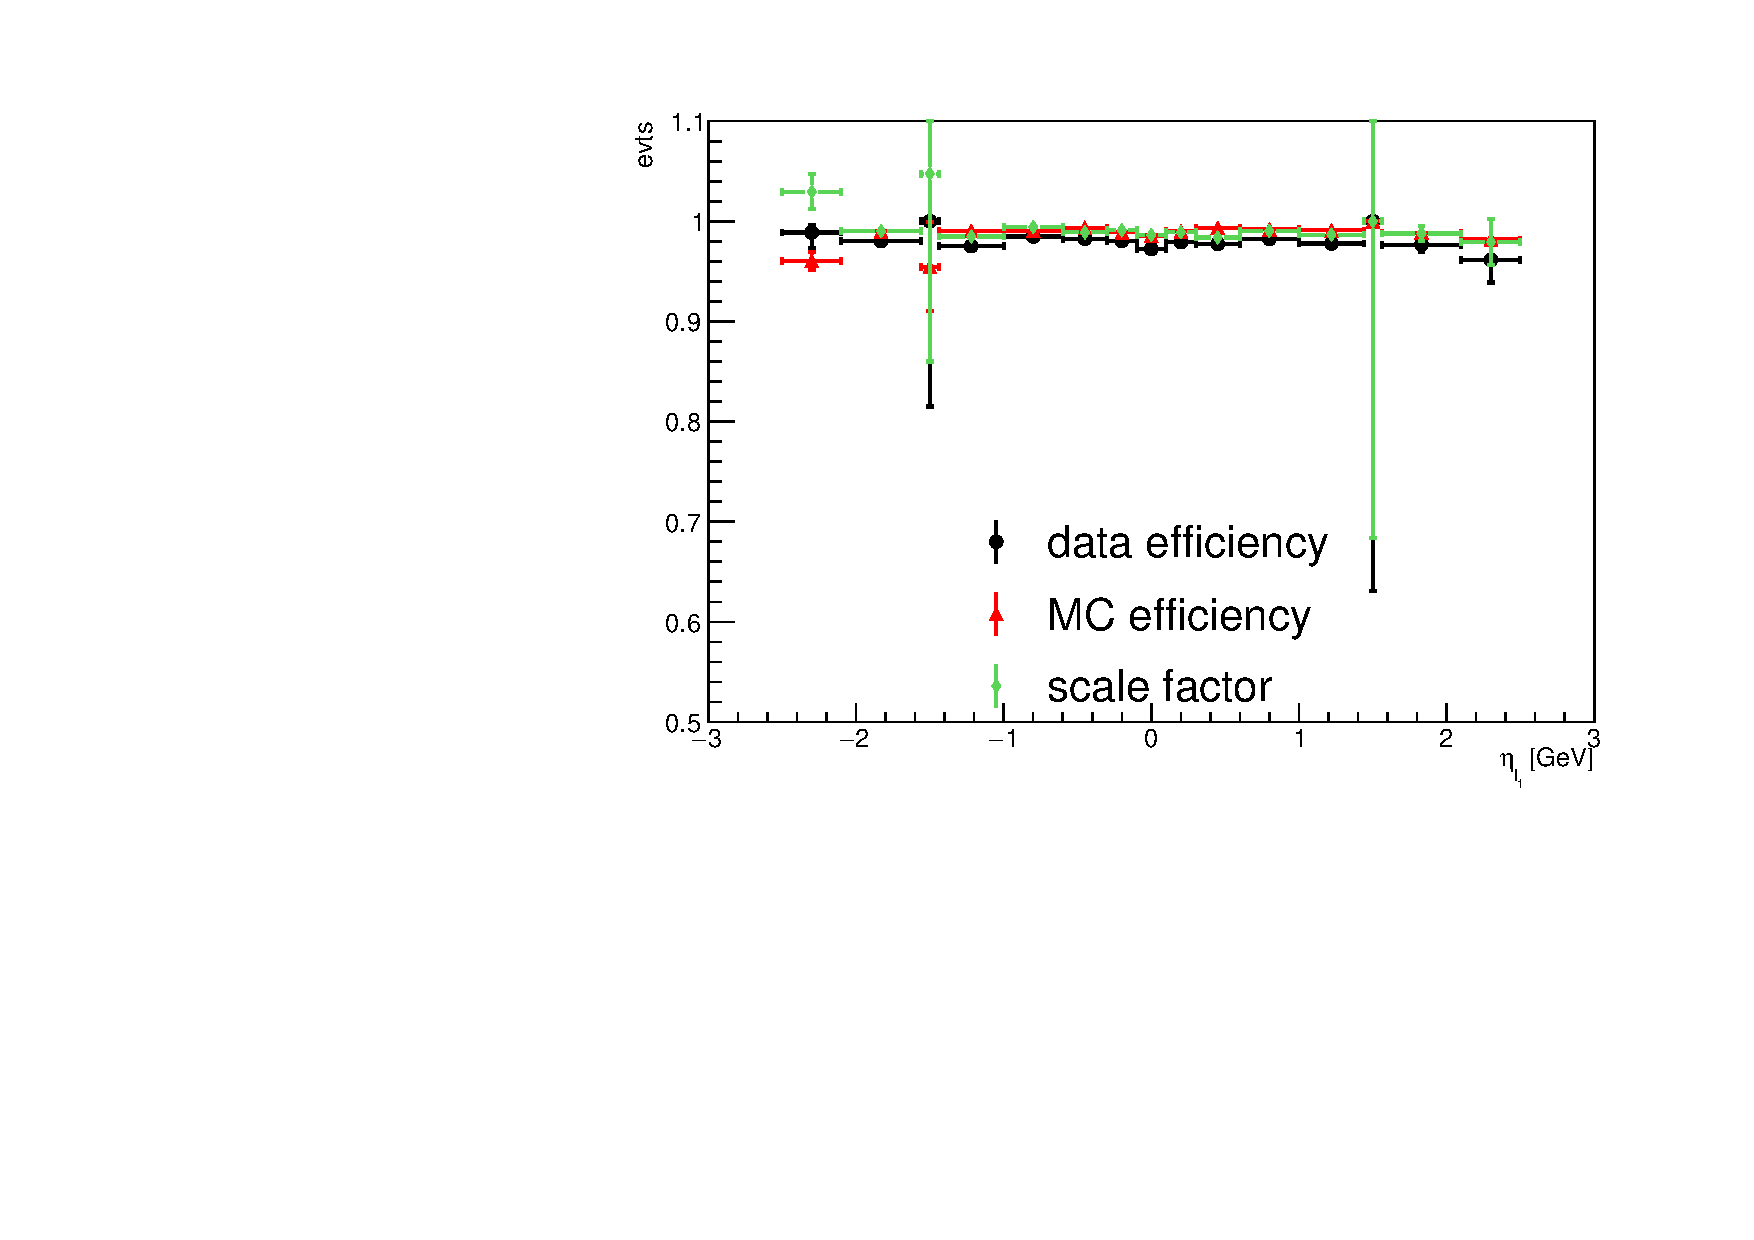
\includegraphics{Trigger/Figures/MET/ee/leading_eta}}
    \resizebox{0.48 \textwidth}{!}{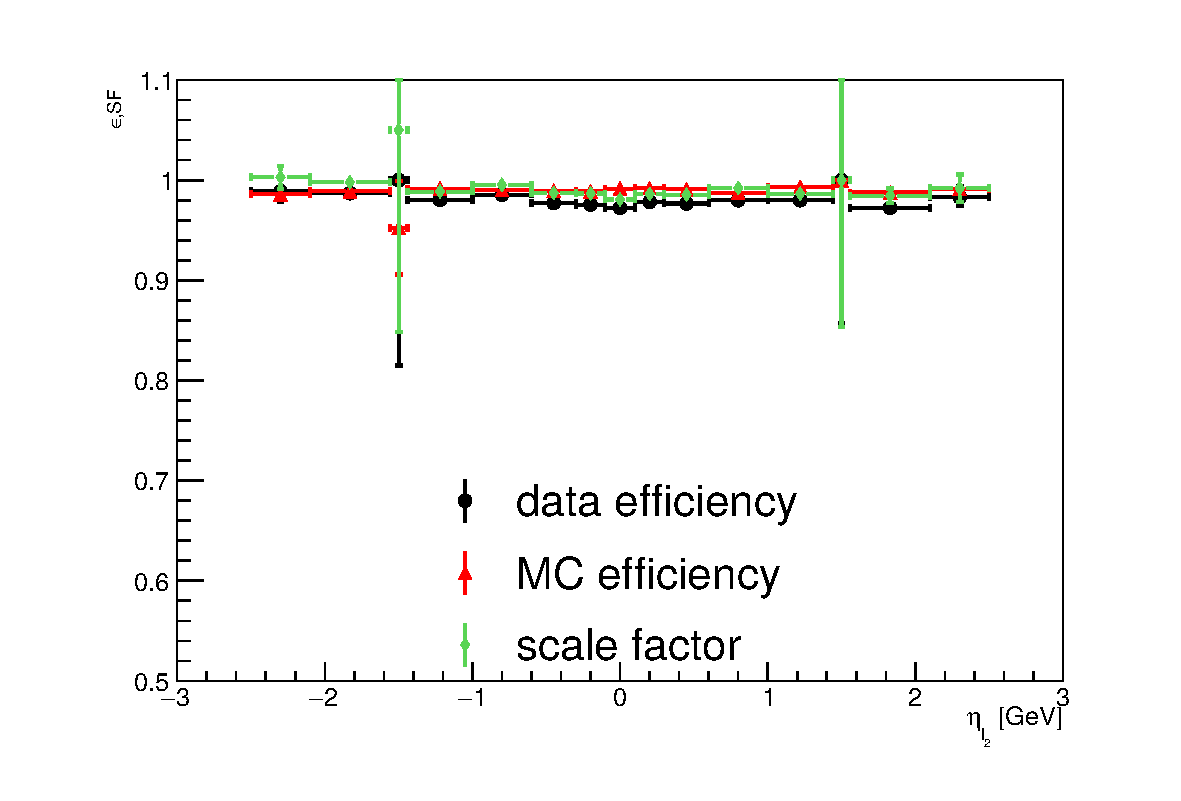
\includegraphics{Trigger/Figures/MET/ee/seleading_eta}}
    \resizebox{0.48 \textwidth}{!}{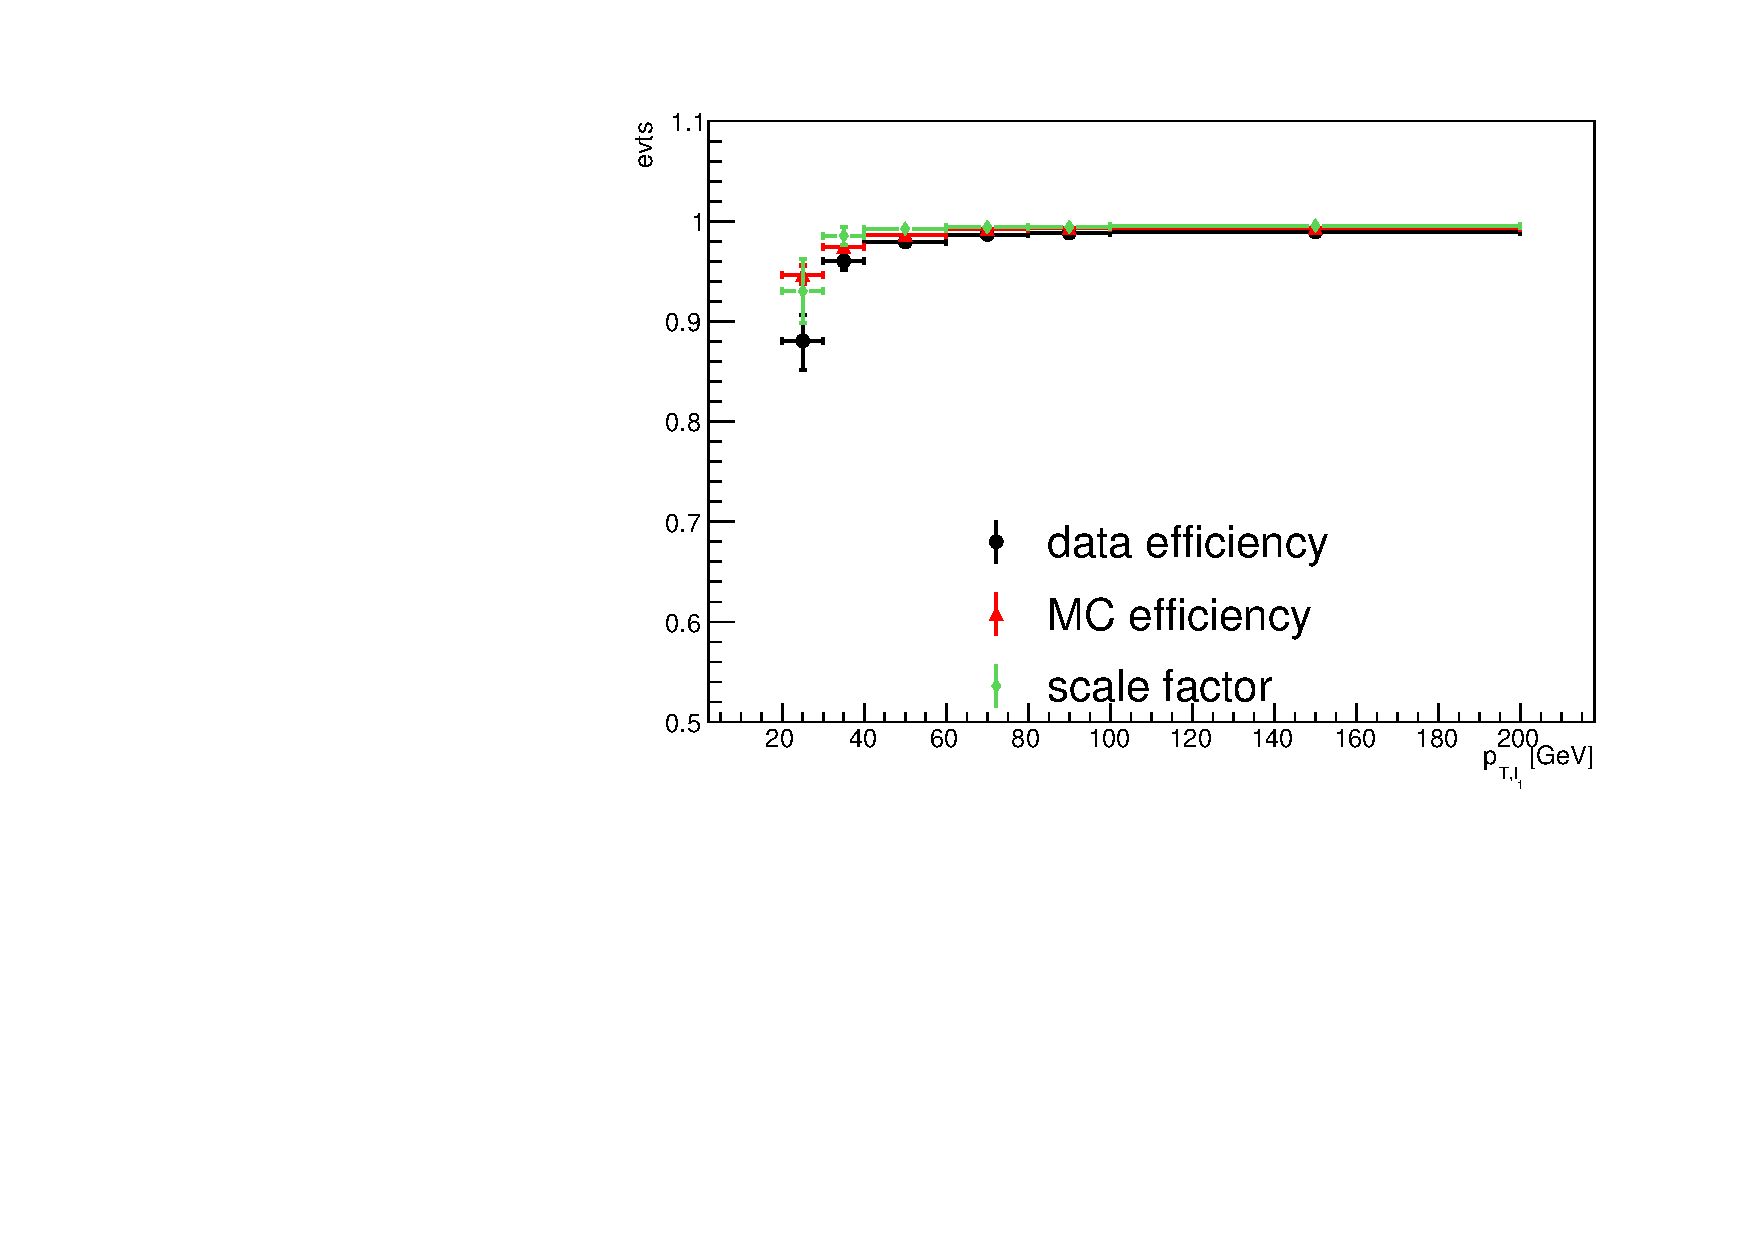
\includegraphics{Trigger/Figures/MET/ee/leading_pt}}
    \resizebox{0.48 \textwidth}{!}{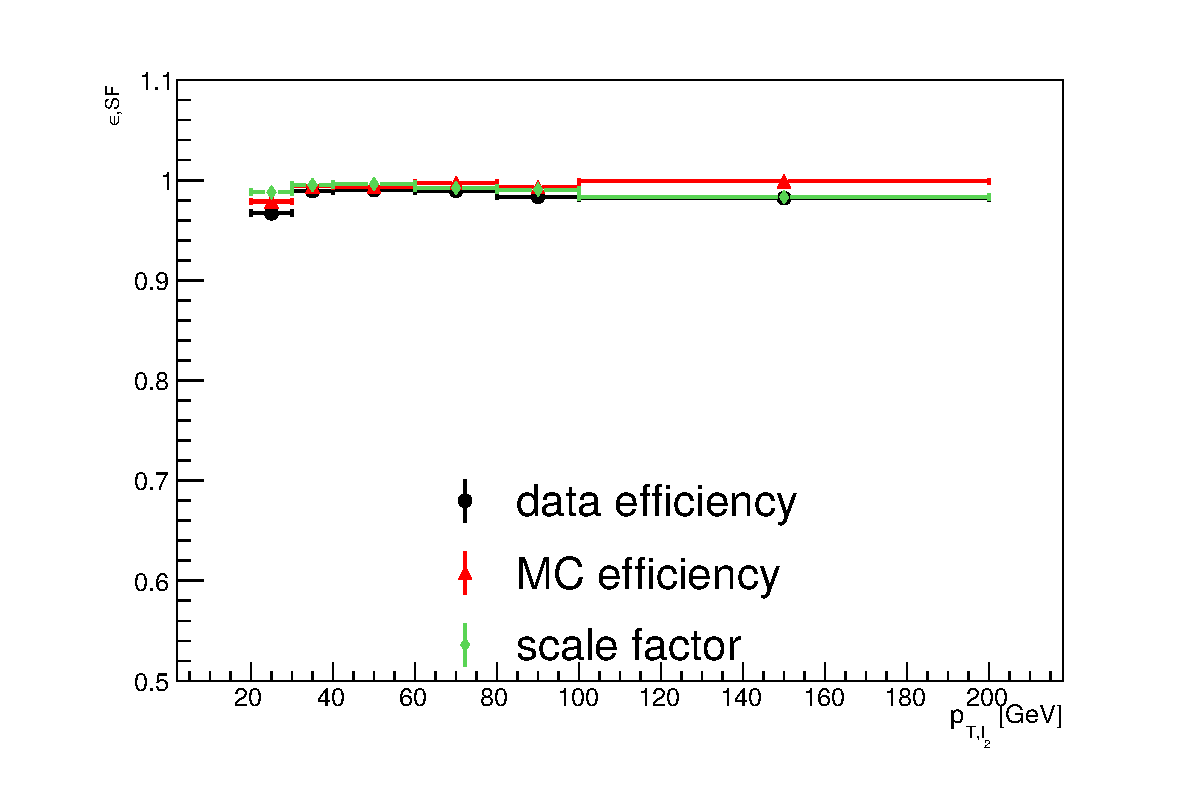
\includegraphics{Trigger/Figures/MET/ee/seleading_pt}}
    \resizebox{0.48 \textwidth}{!}{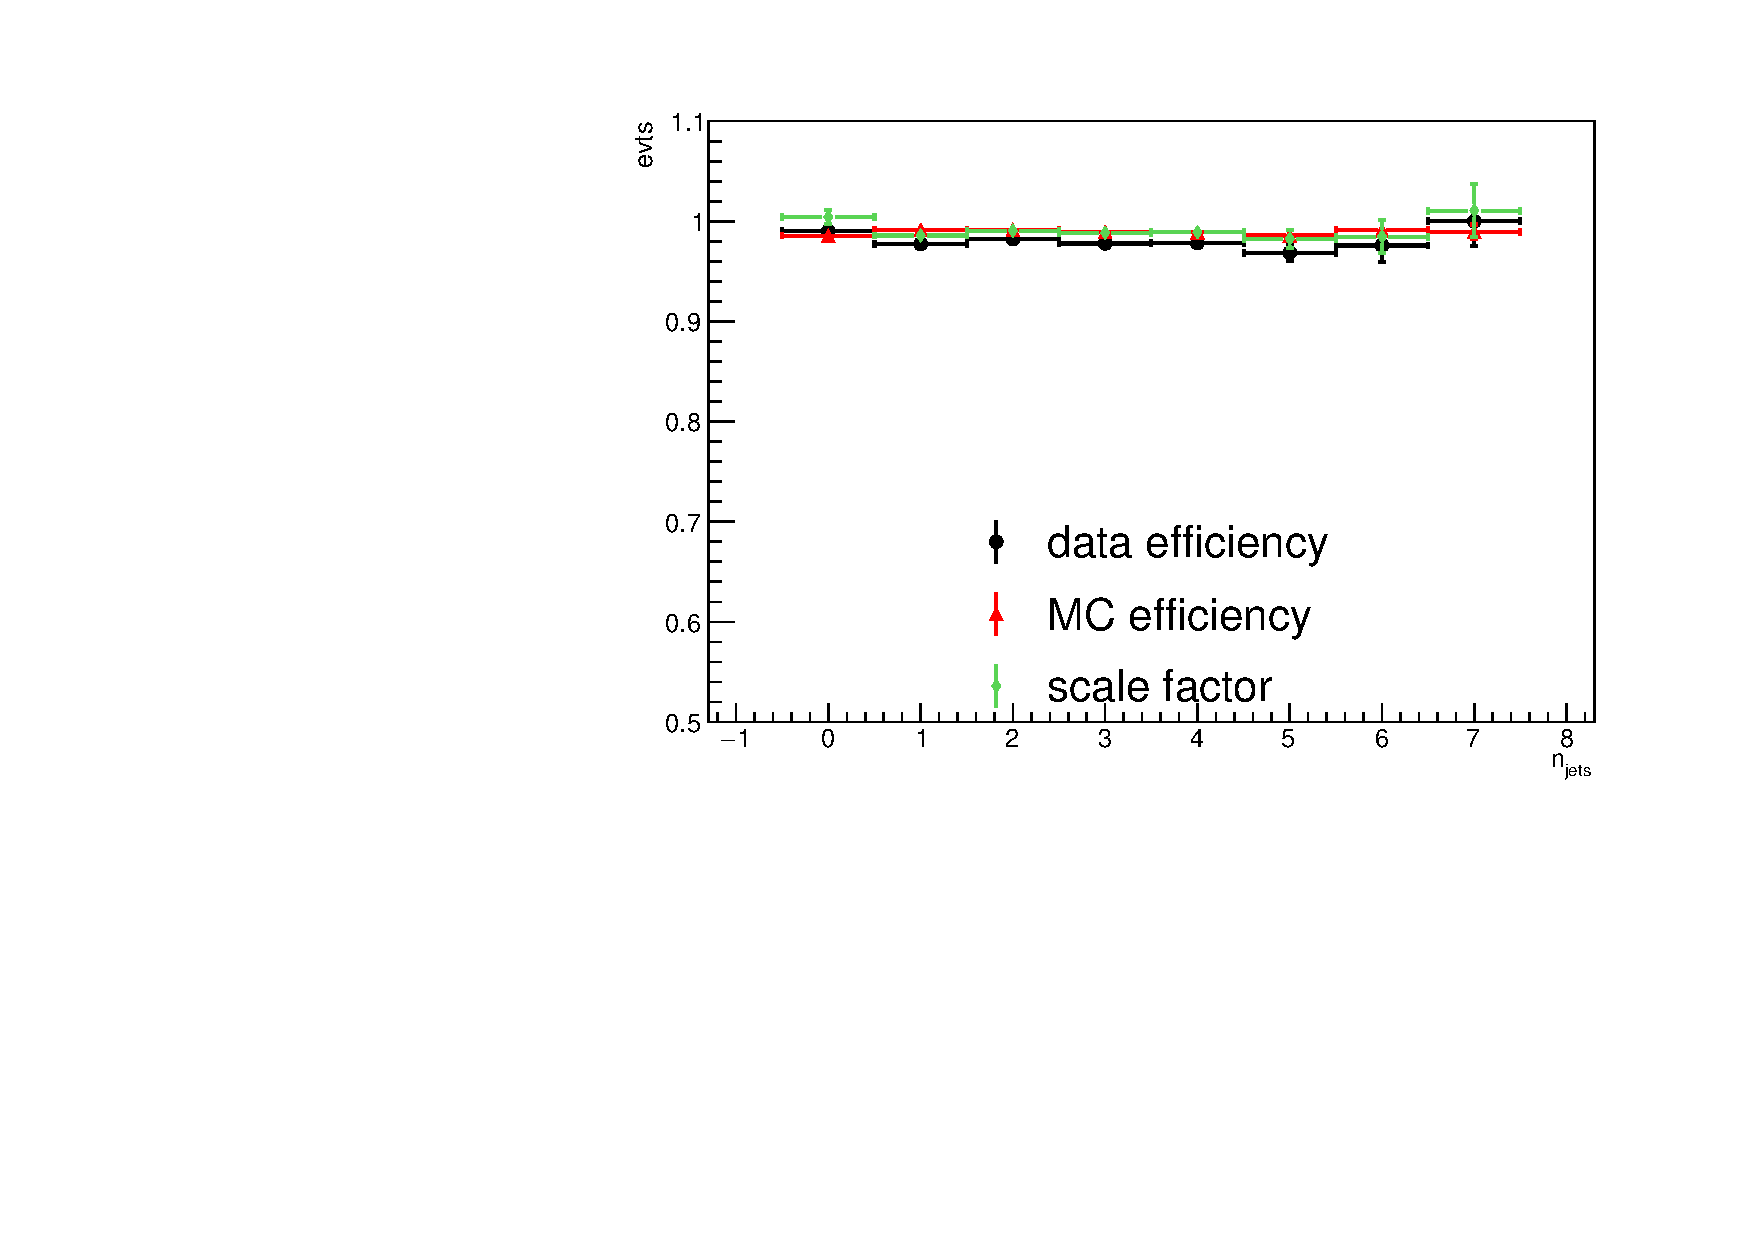
\includegraphics{Trigger/Figures/MET/ee/jet_multi}}
    \resizebox{0.48 \textwidth}{!}{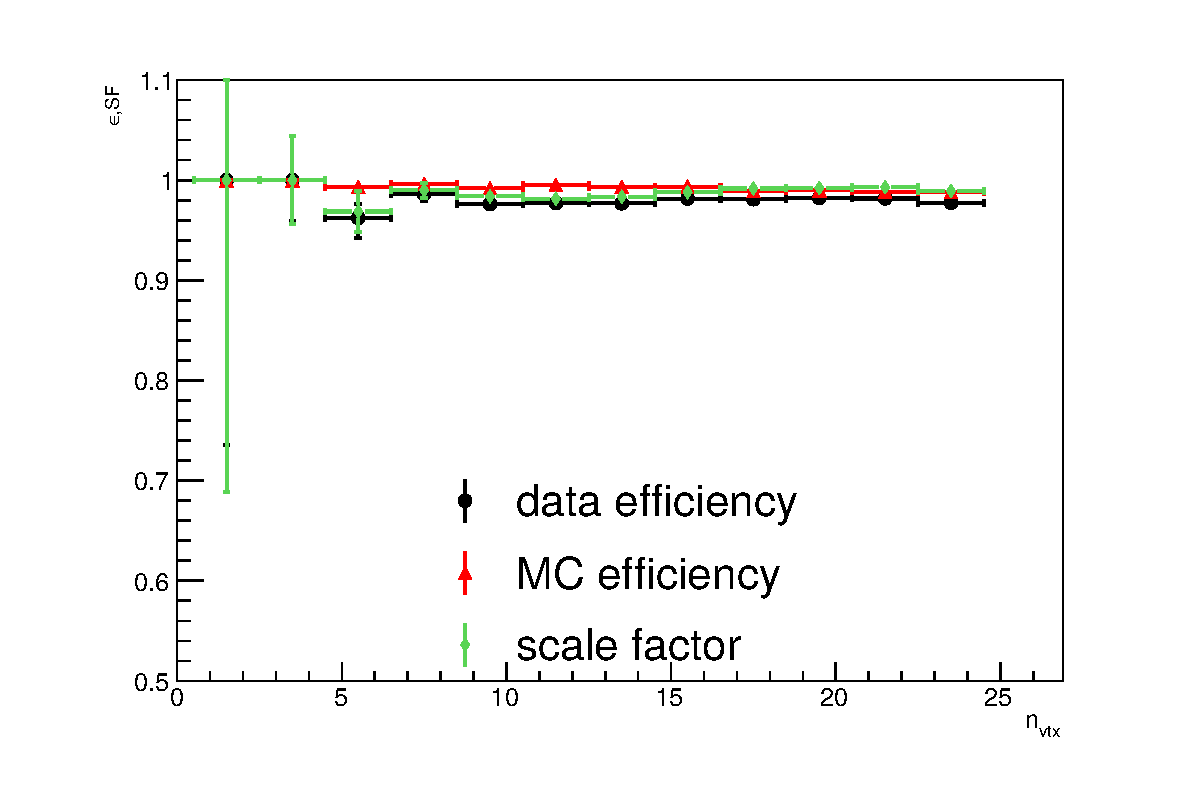
\includegraphics{Trigger/Figures/MET/ee/vertex_multi}}  
      \caption{Efficiencies of the trigger selection in the \ee channel for simulation and data and the corresponding scale factor. The top row shows the efficiency depending on $\eta$ of the leading (left) and trailing (right) lepton. The middle row shows the effciency \pt of the leading (left) and trailing (right) lepton. The bottom rwo shows the efficiency depending on the jet multiplicity on the left and the vertex multiplicity on the right.
       The error bars denote statistical uncertainties. }  
      
    \label{fig:MET_ee}
  \end{center}
\end{figure}

\begin{figure}[htbp!]
  \begin{center}
    \resizebox{0.48 \textwidth}{!}{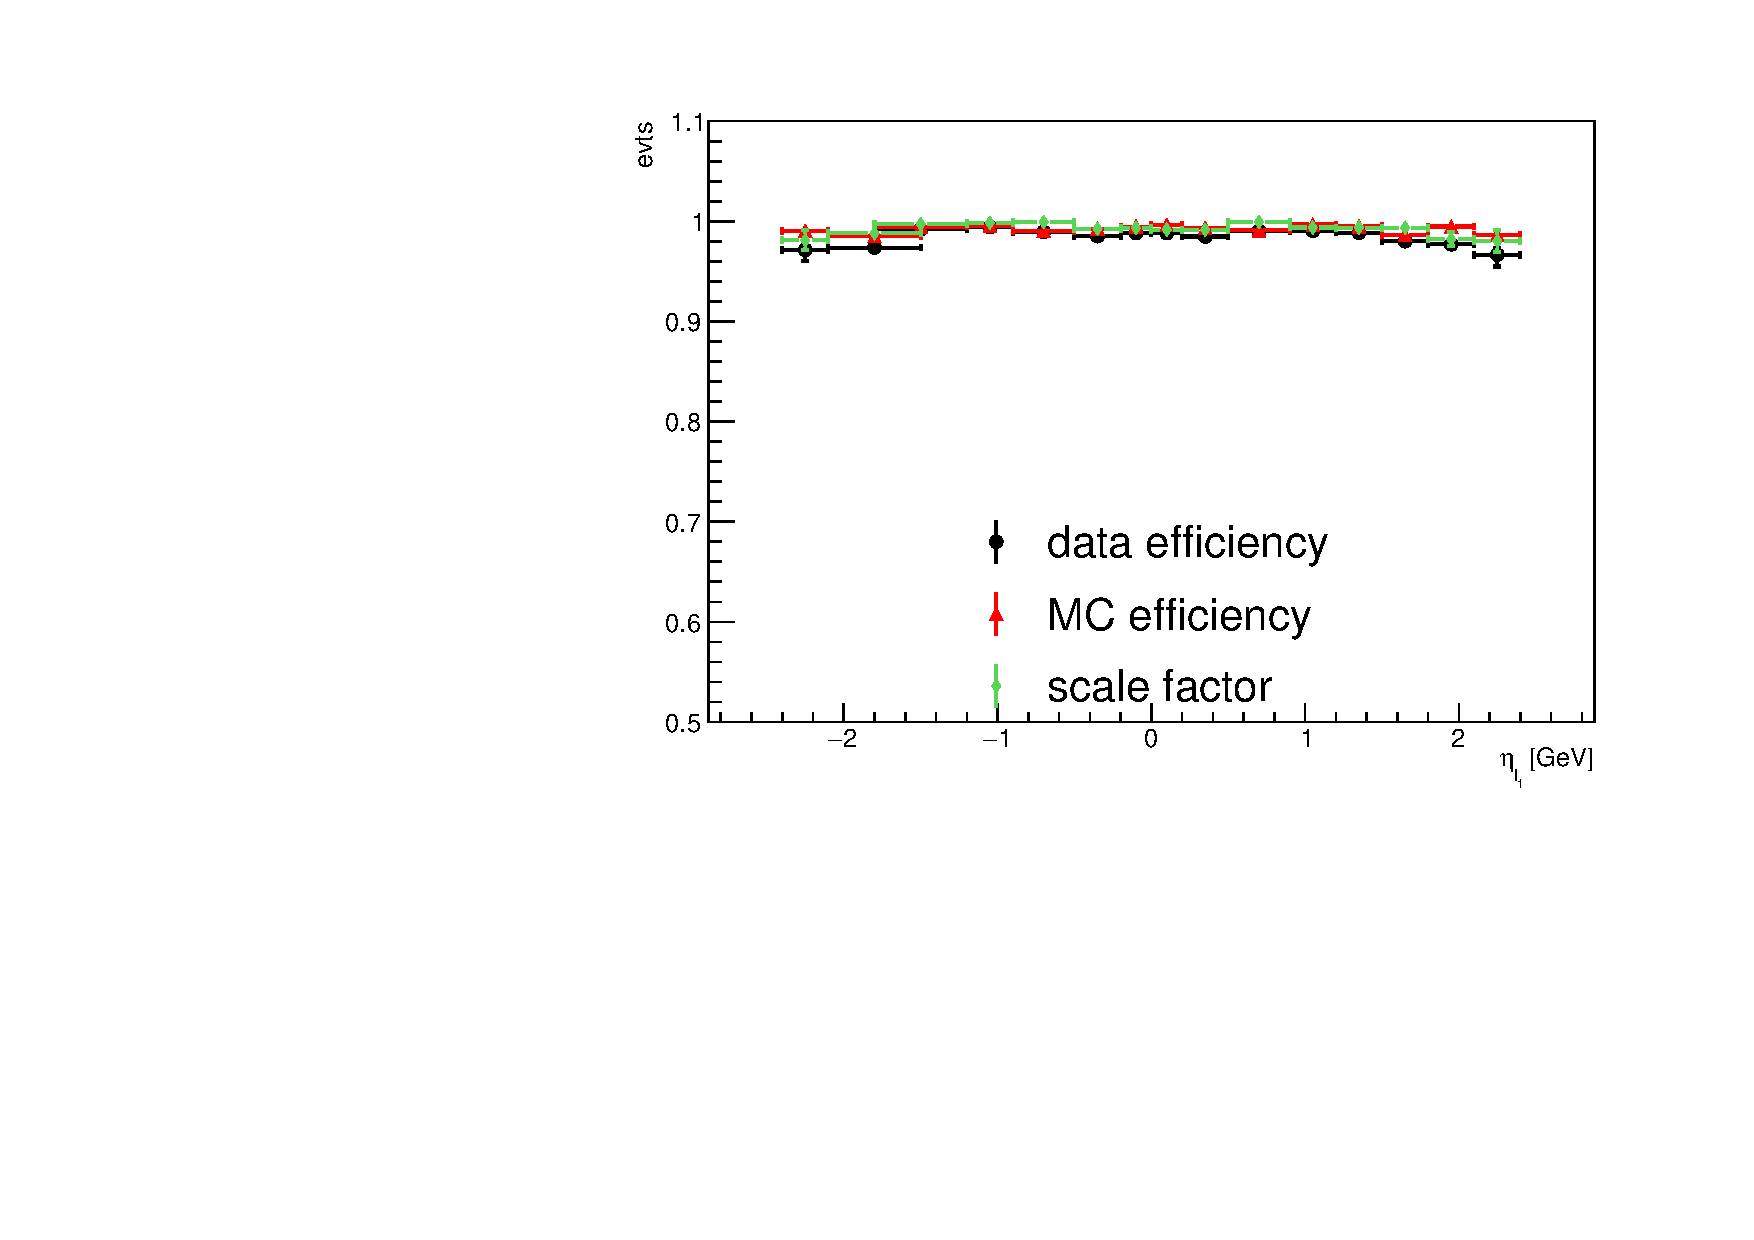
\includegraphics{Trigger/Figures/MET/mumu/leading_eta}}
    \resizebox{0.48 \textwidth}{!}{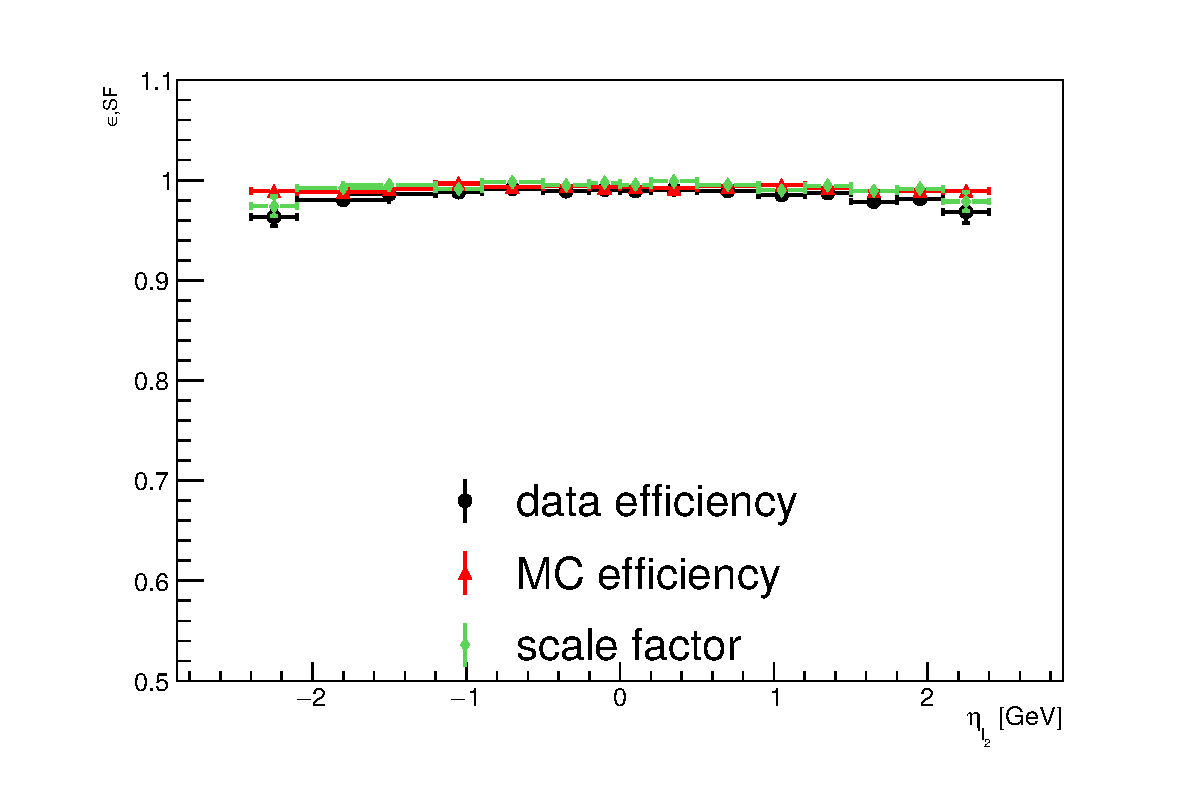
\includegraphics{Trigger/Figures/MET/mumu/seleading_eta}}
    \resizebox{0.48 \textwidth}{!}{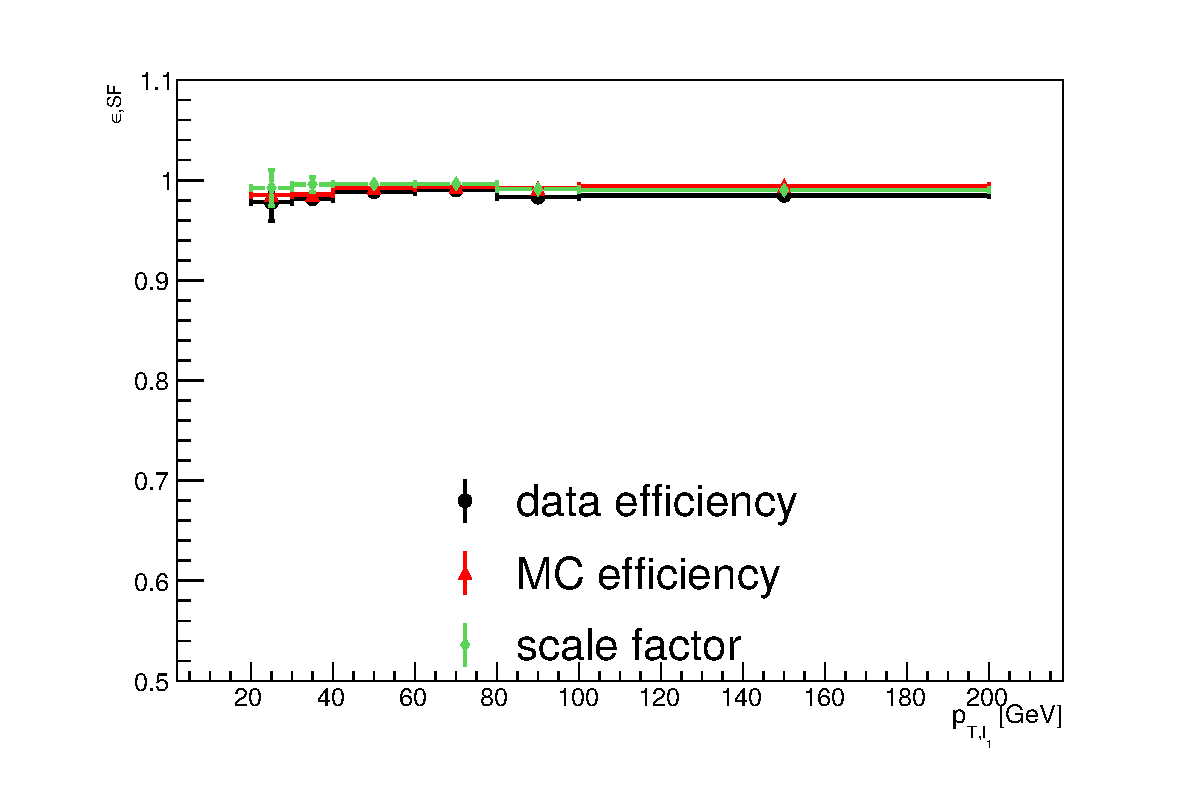
\includegraphics{Trigger/Figures/MET/mumu/leading_pt}}
    \resizebox{0.48 \textwidth}{!}{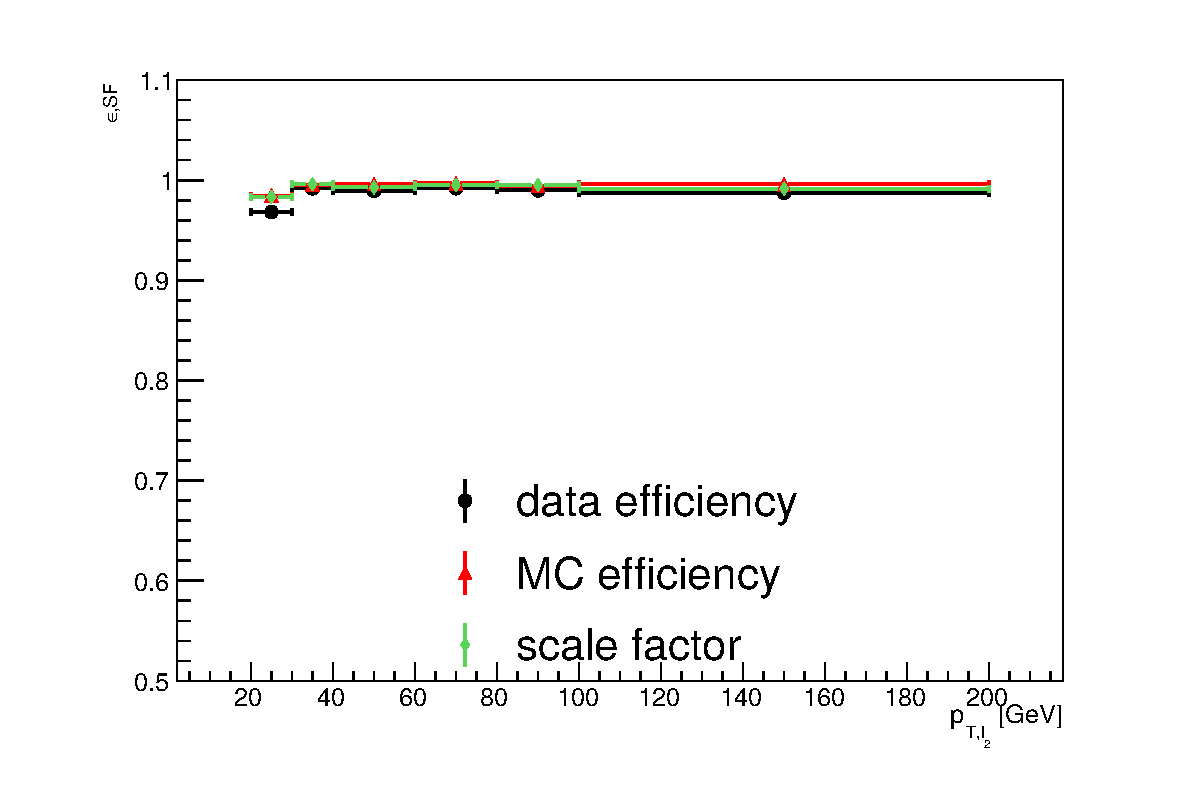
\includegraphics{Trigger/Figures/MET/mumu/seleading_pt}}
    \resizebox{0.48 \textwidth}{!}{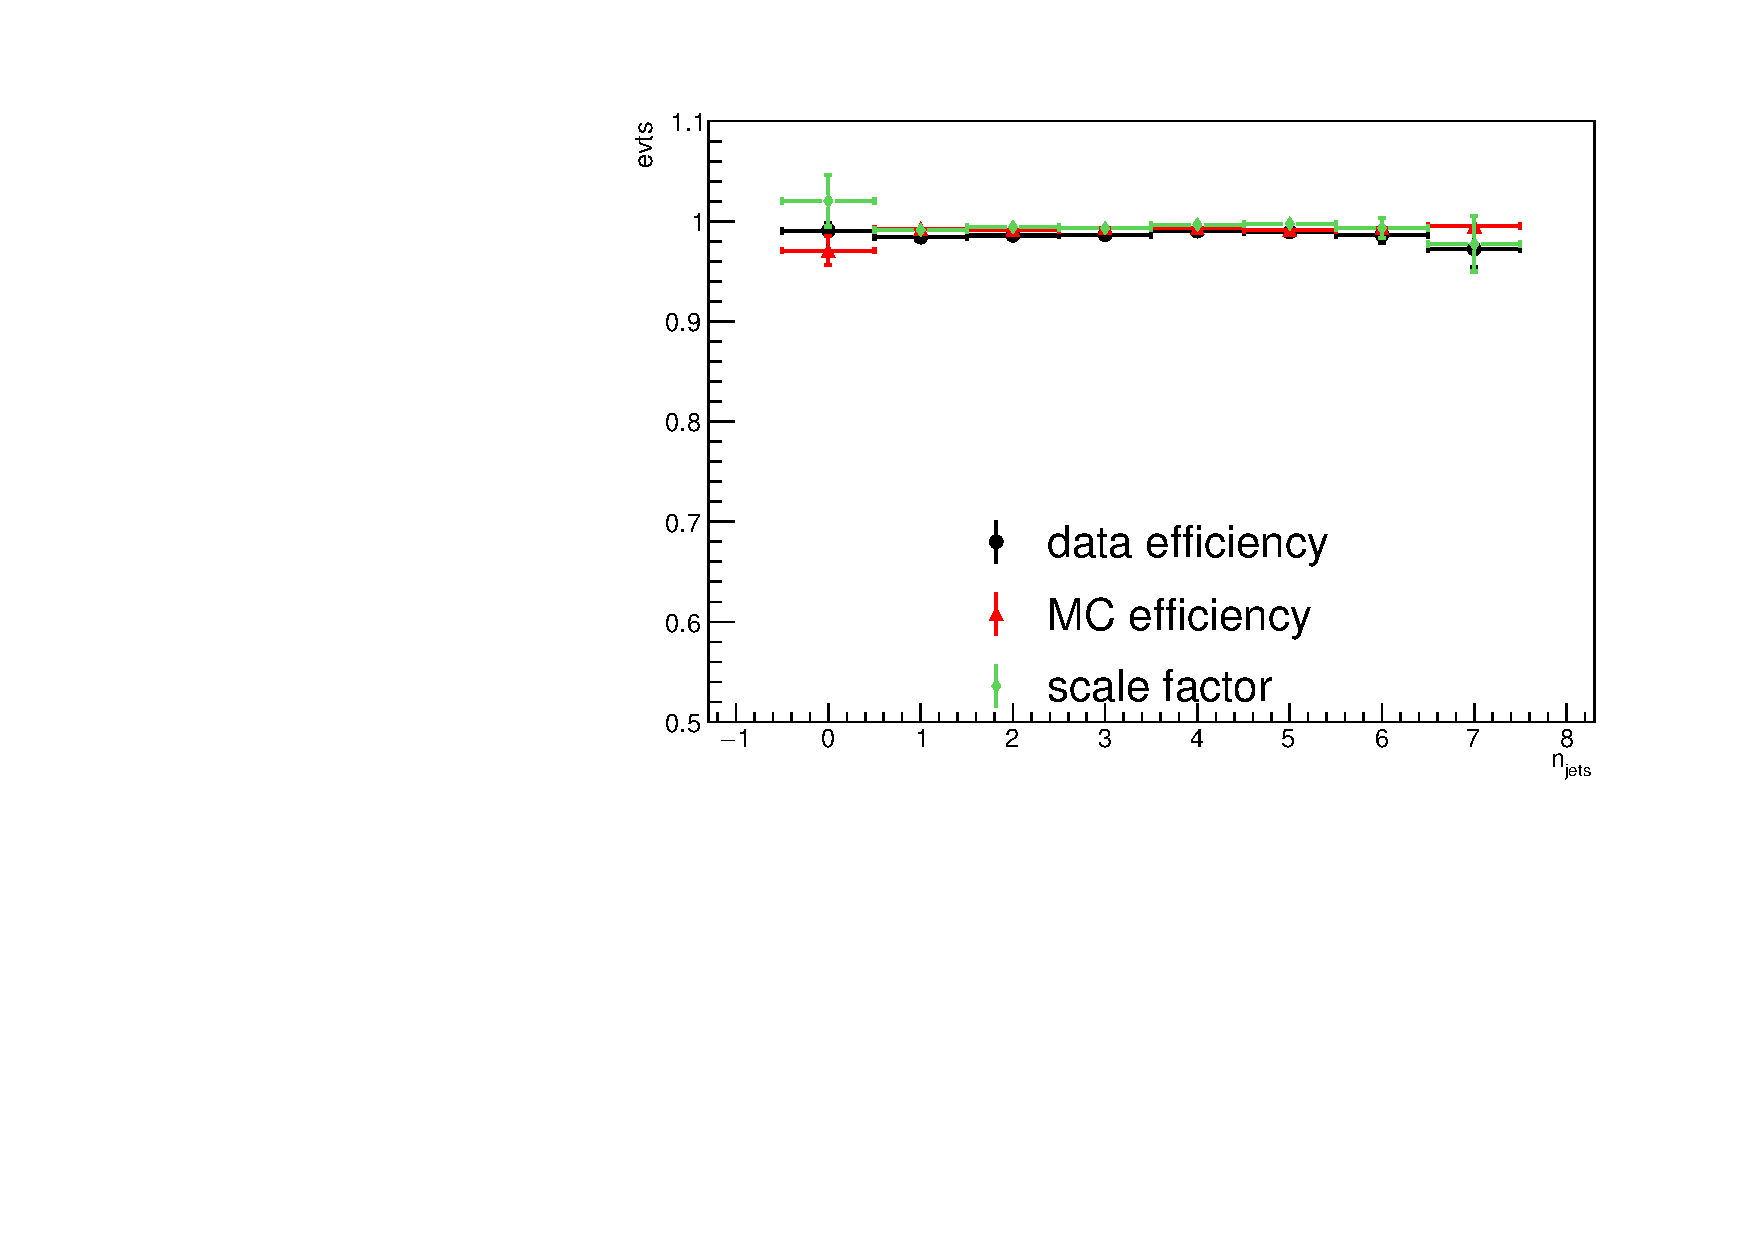
\includegraphics{Trigger/Figures/MET/mumu/jet_multi}}
    \resizebox{0.48 \textwidth}{!}{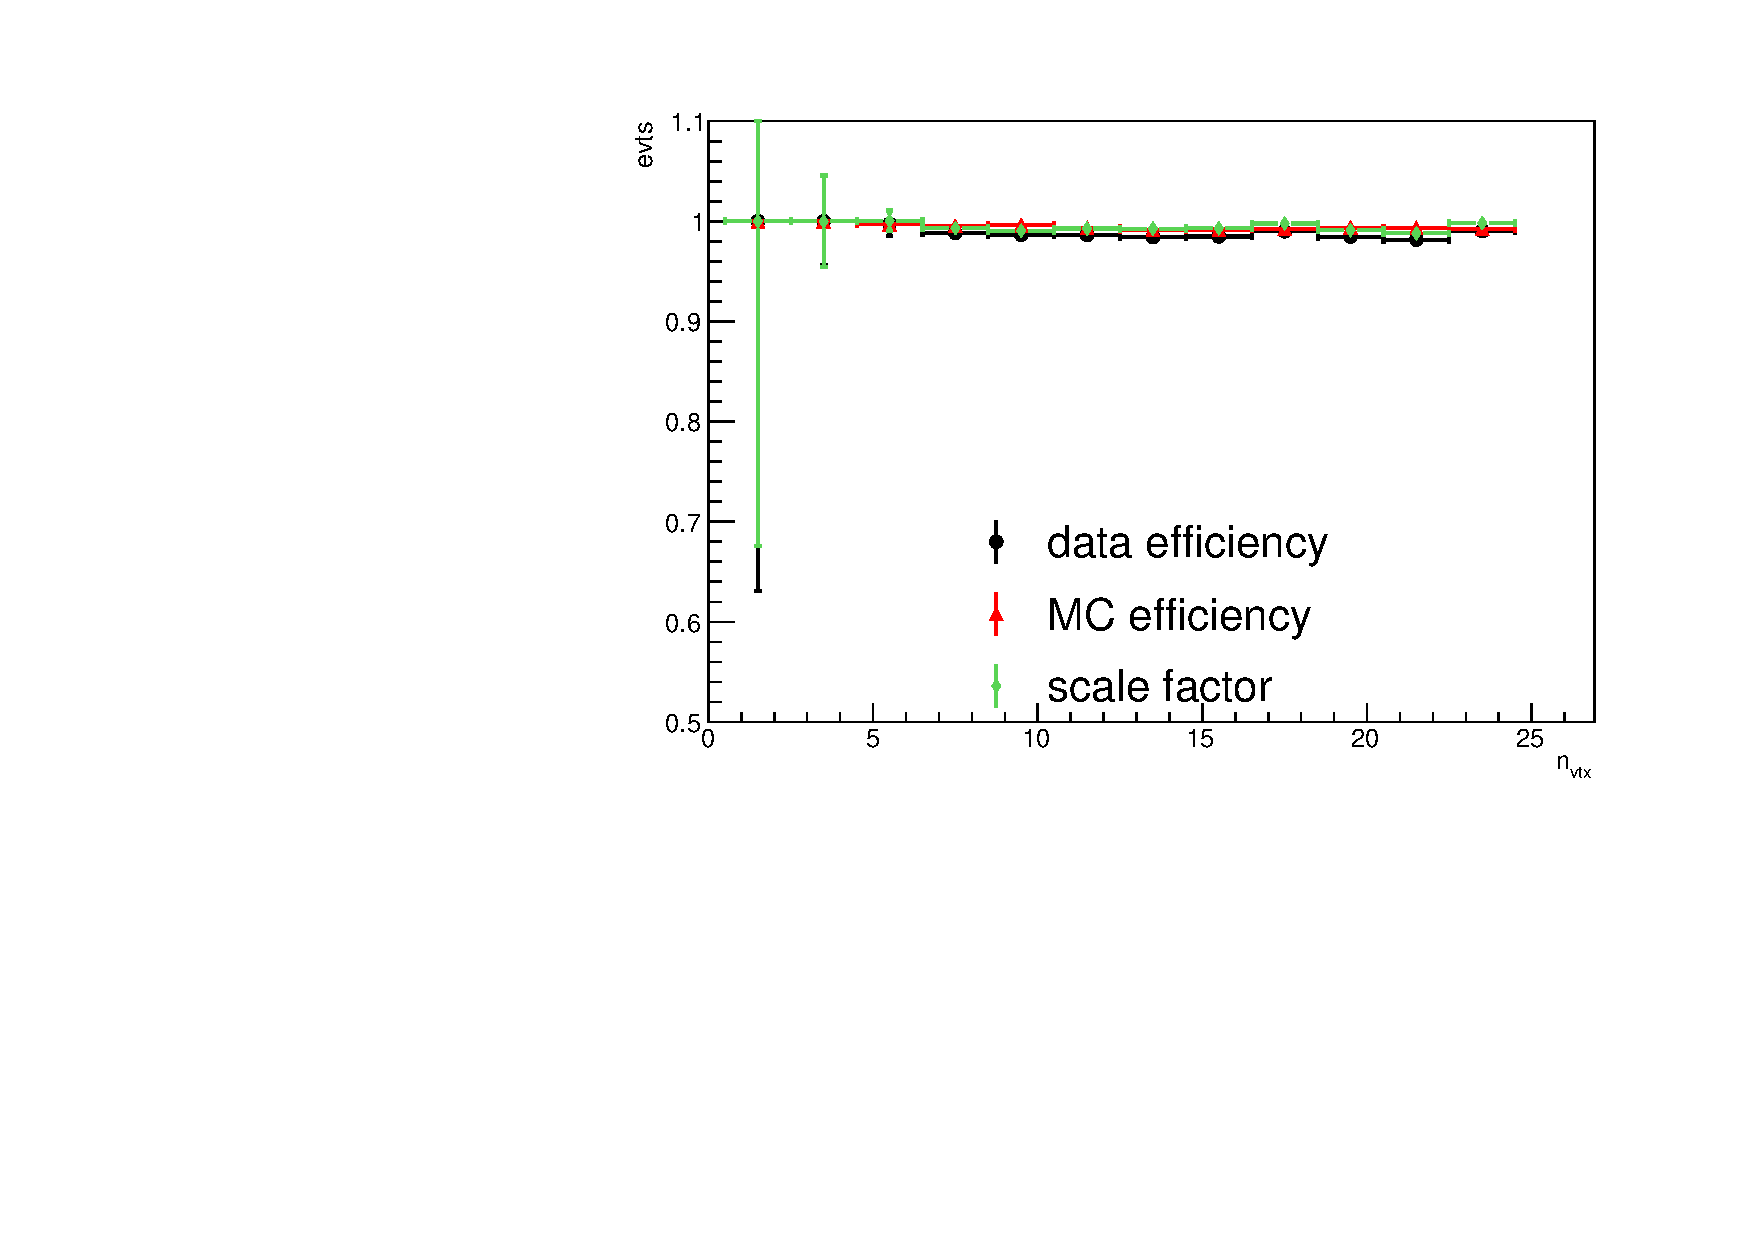
\includegraphics{Trigger/Figures/MET/mumu/vertex_multi}}  
      \caption{Efficiencies of the trigger selection in the \mumu channel for simulation and data and the corresponding scale factor. The top row shows the efficiency depending on $\eta$ of the leading (left) and trailing (right) lepton. The middle row shows the effciency \pt of the leading (left) and trailing (right) lepton. The bottom rwo shows the efficiency depending on the jet multiplicity on the left and the vertex multiplicity on the right.
      The error bars denote statistical uncertainties. }  
      
    \label{fig:MET_mumu}
  \end{center}
\end{figure}

\begin{figure}[htbp!]
  \begin{center}
    \resizebox{0.48 \textwidth}{!}{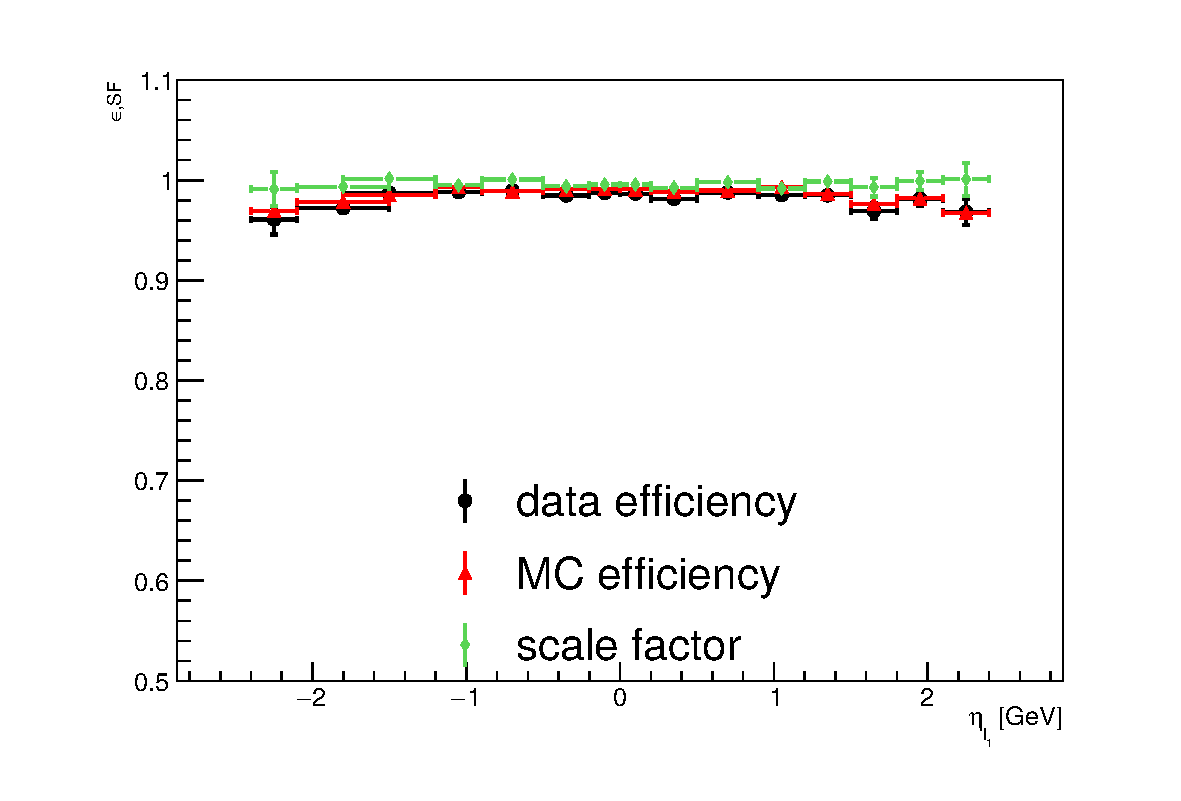
\includegraphics{Trigger/Figures/MET/emu/leading_eta}}
    \resizebox{0.48 \textwidth}{!}{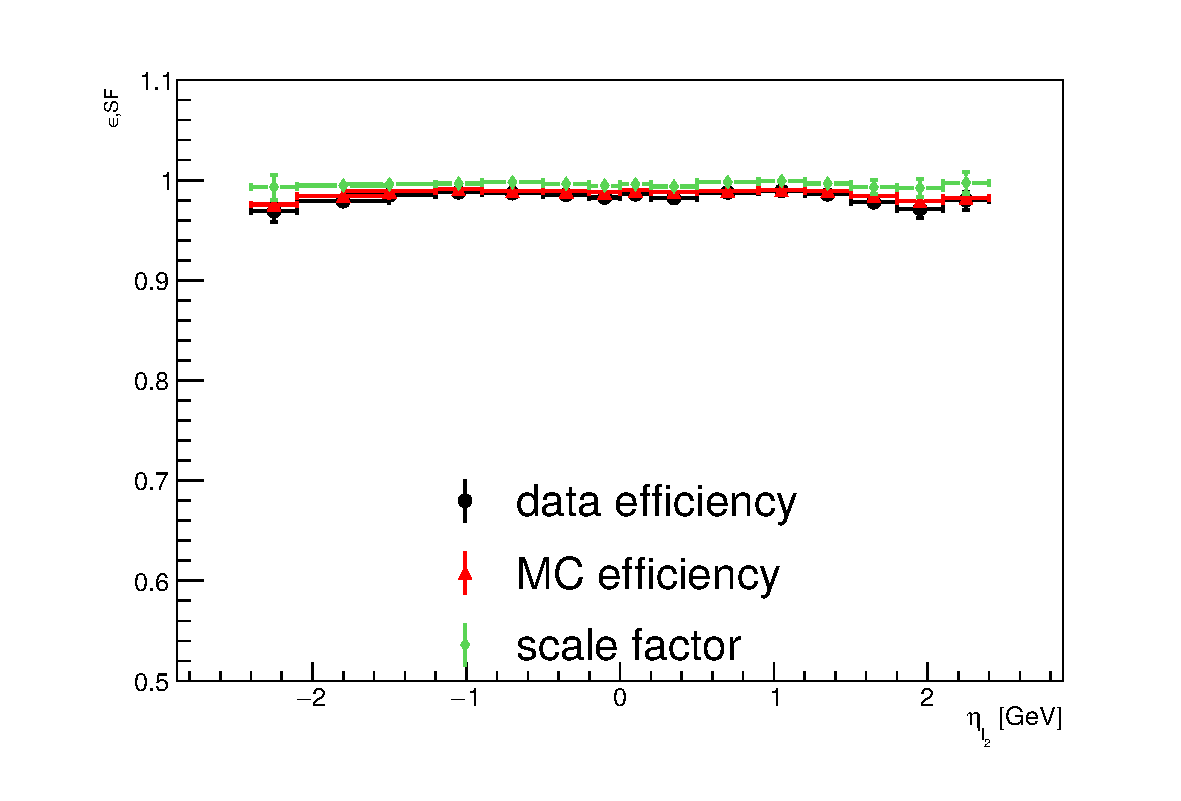
\includegraphics{Trigger/Figures/MET/emu/seleading_eta}}
    \resizebox{0.48 \textwidth}{!}{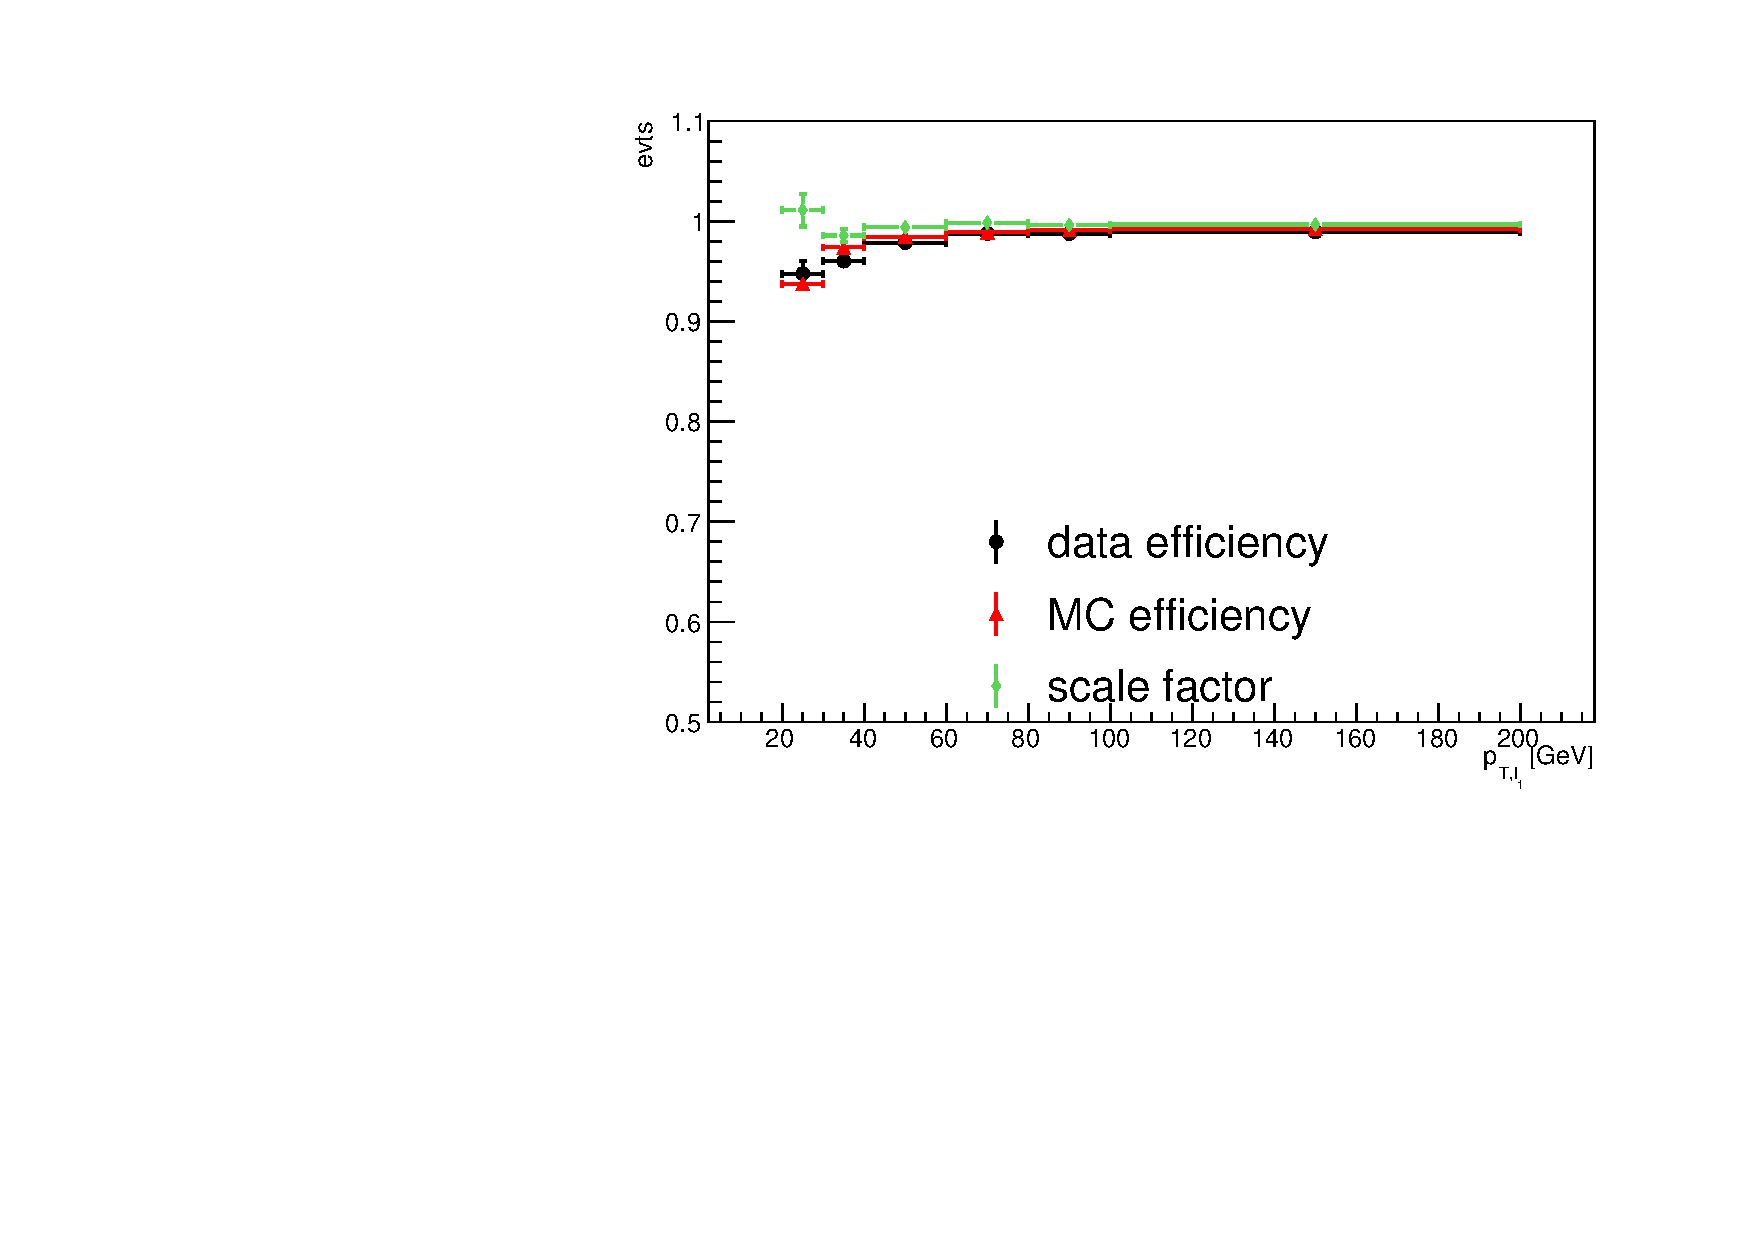
\includegraphics{Trigger/Figures/MET/emu/leading_pt}}
    \resizebox{0.48 \textwidth}{!}{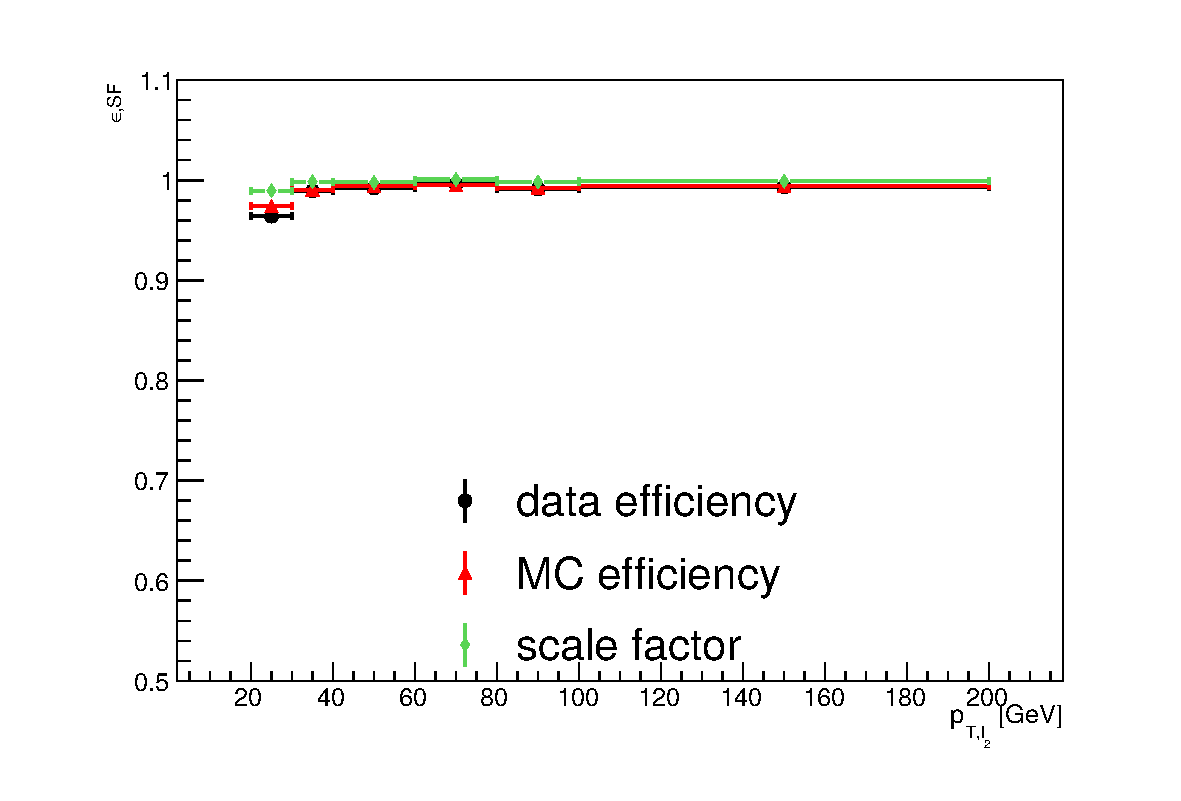
\includegraphics{Trigger/Figures/MET/emu/seleading_pt}}
    \resizebox{0.48 \textwidth}{!}{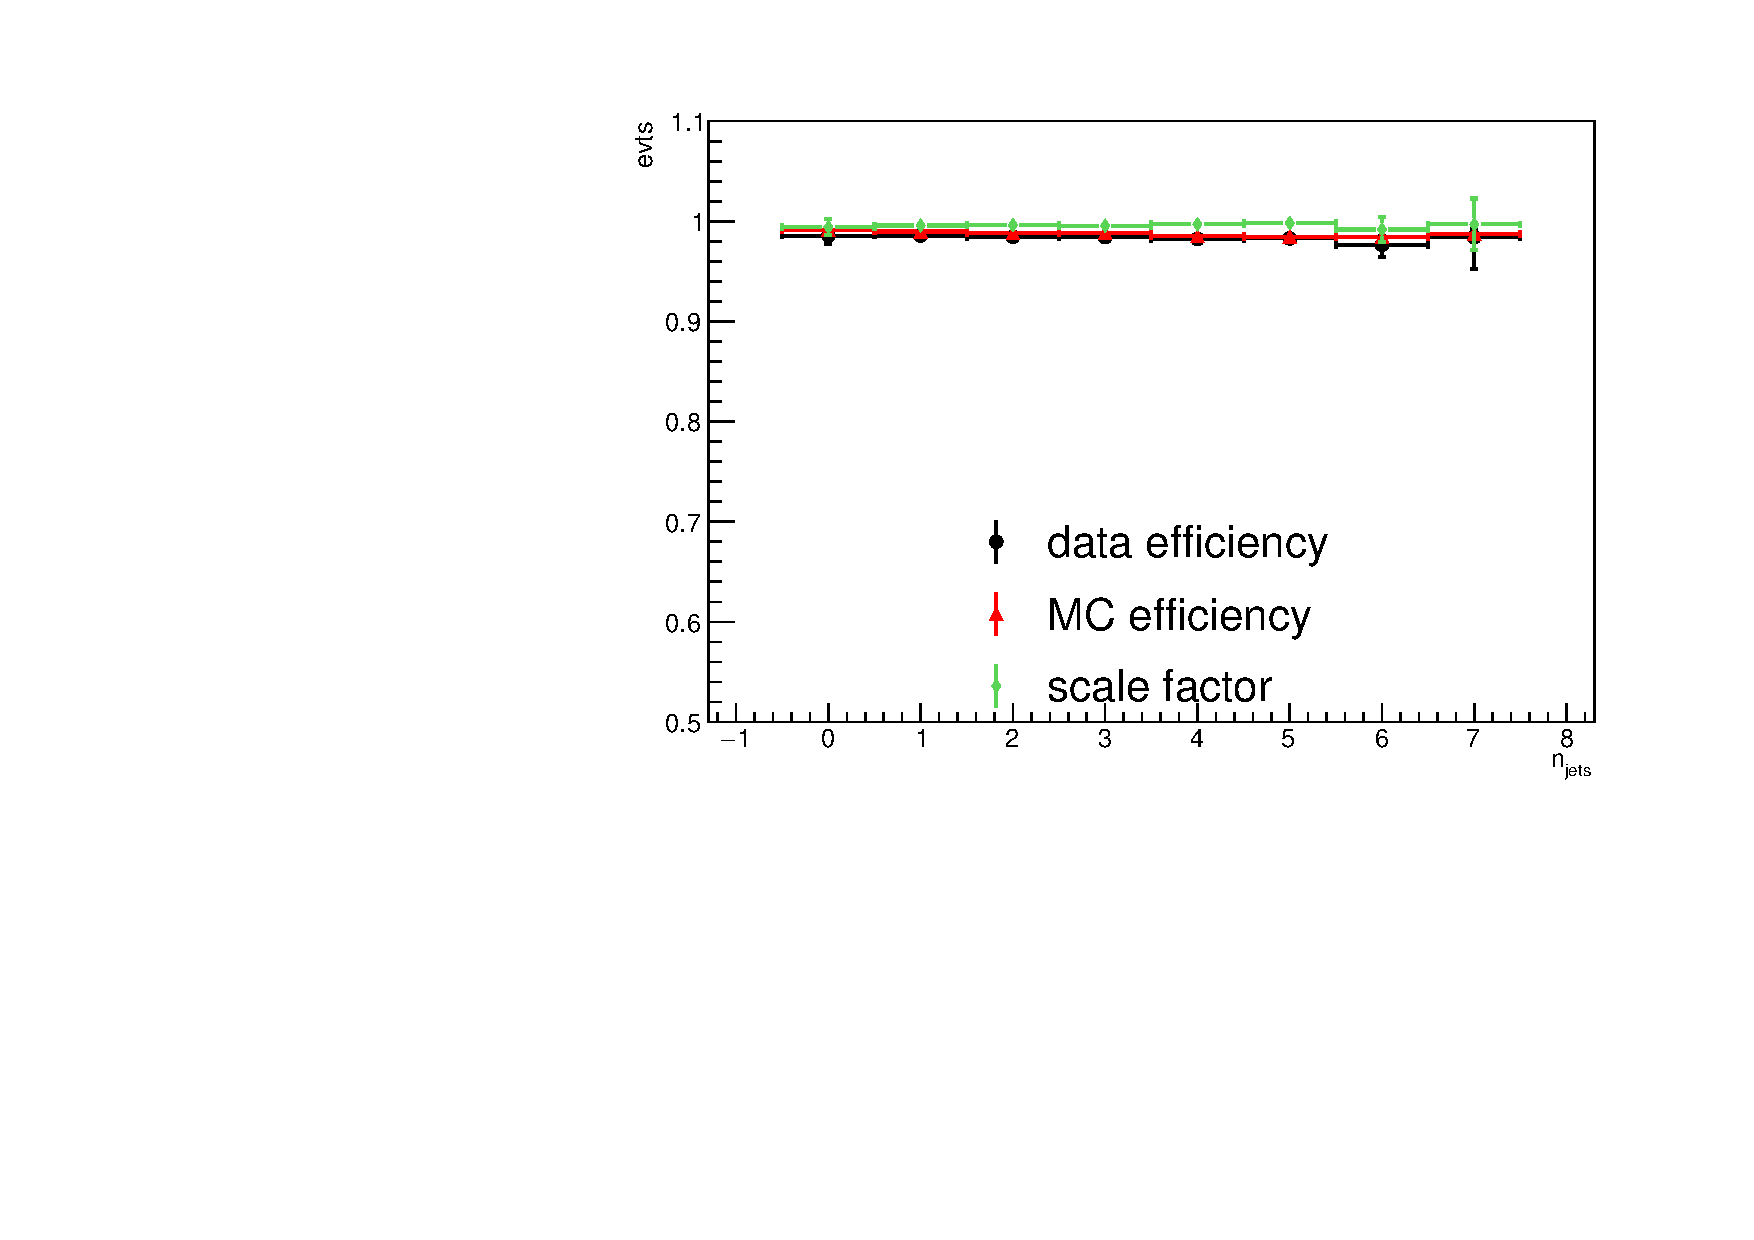
\includegraphics{Trigger/Figures/MET/emu/jet_multi}}
    \resizebox{0.48 \textwidth}{!}{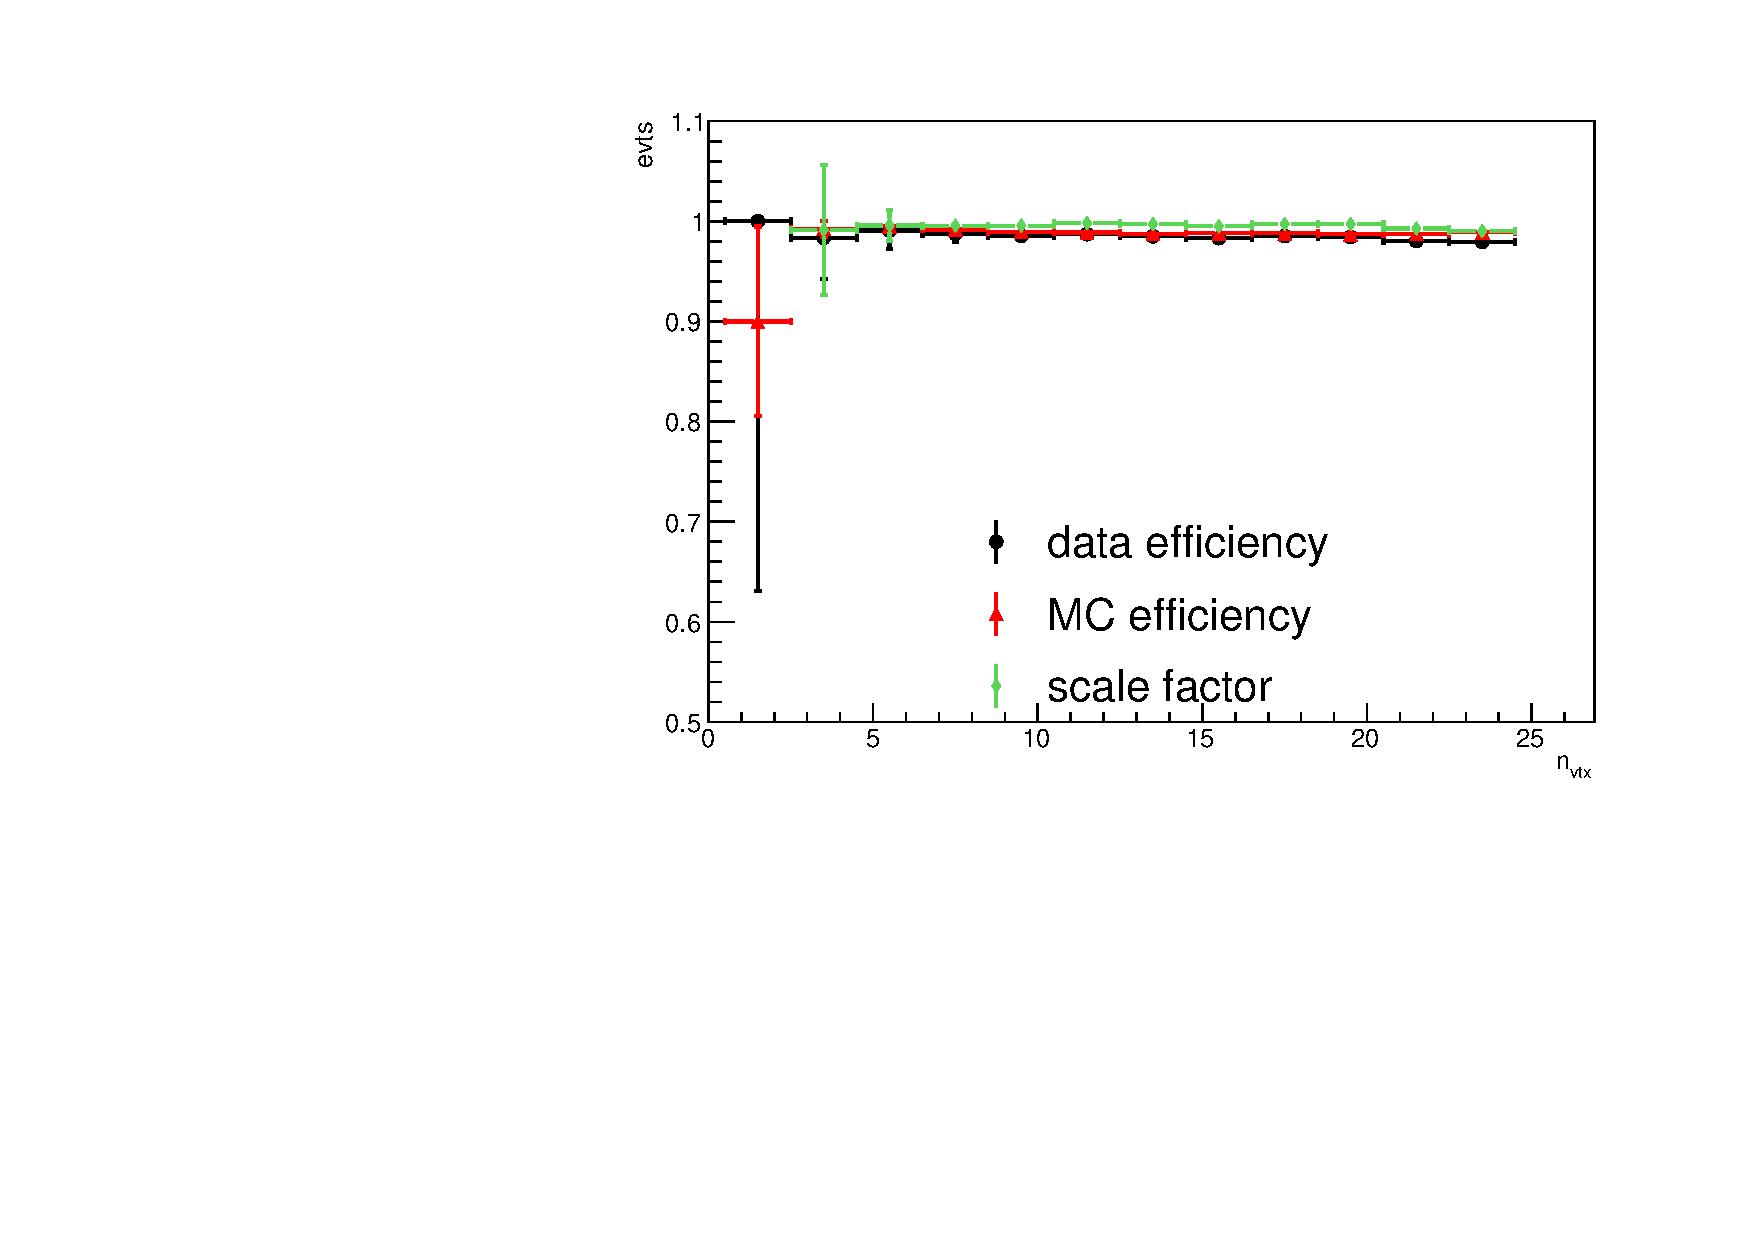
\includegraphics{Trigger/Figures/MET/emu/vertex_multi}}  
      \caption{Efficiencies of the trigger selection in the \emu channel for simulation and data and the corresponding scale factor. The top row shows the efficiency depending on $\eta$ of the leading (left) and trailing (right) lepton. The middle row shows the effciency \pt of the leading (left) and trailing (right) lepton. The bottom rwo shows the efficiency depending on the jet multiplicity on the left and the vertex multiplicity on the right.
      The error bars denote statistical uncertainties. }  
      
    \label{fig:MET_emu}
  \end{center}
\end{figure}


%********************************** % Third Section  *************************************
\section{Method: Tag and Probe}  %Section - 1.3 
\label{sec:TriggerTPMethod}

In order to provide an alternative and totally independent trigger efficiency measurement the Tag and Probe method is used.
Here the trigger efficiency can be measured independently in data and simulation by using the decay of the Z-boson into two leptons.

In general one of the leptons (the Tag) is required to pass a tight selection. This selection includes matching the offline lepton to the lepton reconstructed at trigger level by requiring the two to have a maximum distance and difference in \pt. The second lepton (the Probe) is only required to pass a very loose selection, so it should be as unbiased as possible. The invariant mass of the two leptons then needs to be within the Z-mass window, in which case it can generally be assumed that the leptons are real leptons and not fakes.
In order to measure the efficiency of a certain requirement the probe can then either fullfill it ("passing probe") or fail it ("failing probe"). The efficiency is then determined by dividing the number of passing probes by all probes.

A residual fake contamination is determined by fitting both background and signal distributions for passing and failing probes. The background distribution is often described by an exponential function. The signal has a more complicated functional form, it can for example be parametrized by a double voigtian function. When the efficiency is measured on data it is also possible to fit templates from MC.
In contrast for the efficiency determination in simulation a fit is sometimes not needed as the fake contamination can be negligible.

The efficiency is measured differentialy depending on kinematic properties of the lepton. It commonly depends on both the $\eta$ and the \pt of the lepton. 

In contrast to the efficiency measurement using orthogonal triggers (see Section \ref{sec:TriggerMetMethod}) the Tag and Probe measurement depends on a specific lepton. It measures the efficiency for each lepton, consequently several measurements have to be combined for a multi lepton trigger or an efficiency measurement with multiple triggers (see Section \ref{sec:TriggerComp}). 

Examples for the efficiency measurement in one bin as well as the overall scale factor for the muonic part ("muon leg") of the\\ HLT\_Mu23\_TrkIsoVVL\_Ele12\_CaloIdL\_TrackIdL\_IsoVL trigger both for data and simulation and the resulting overall scale factors are shown in Figure \ref{fig:TP_Mu23}.

\begin{figure}[htbp!]
  \begin{center}
    \resizebox{0.48 \textwidth}{!}{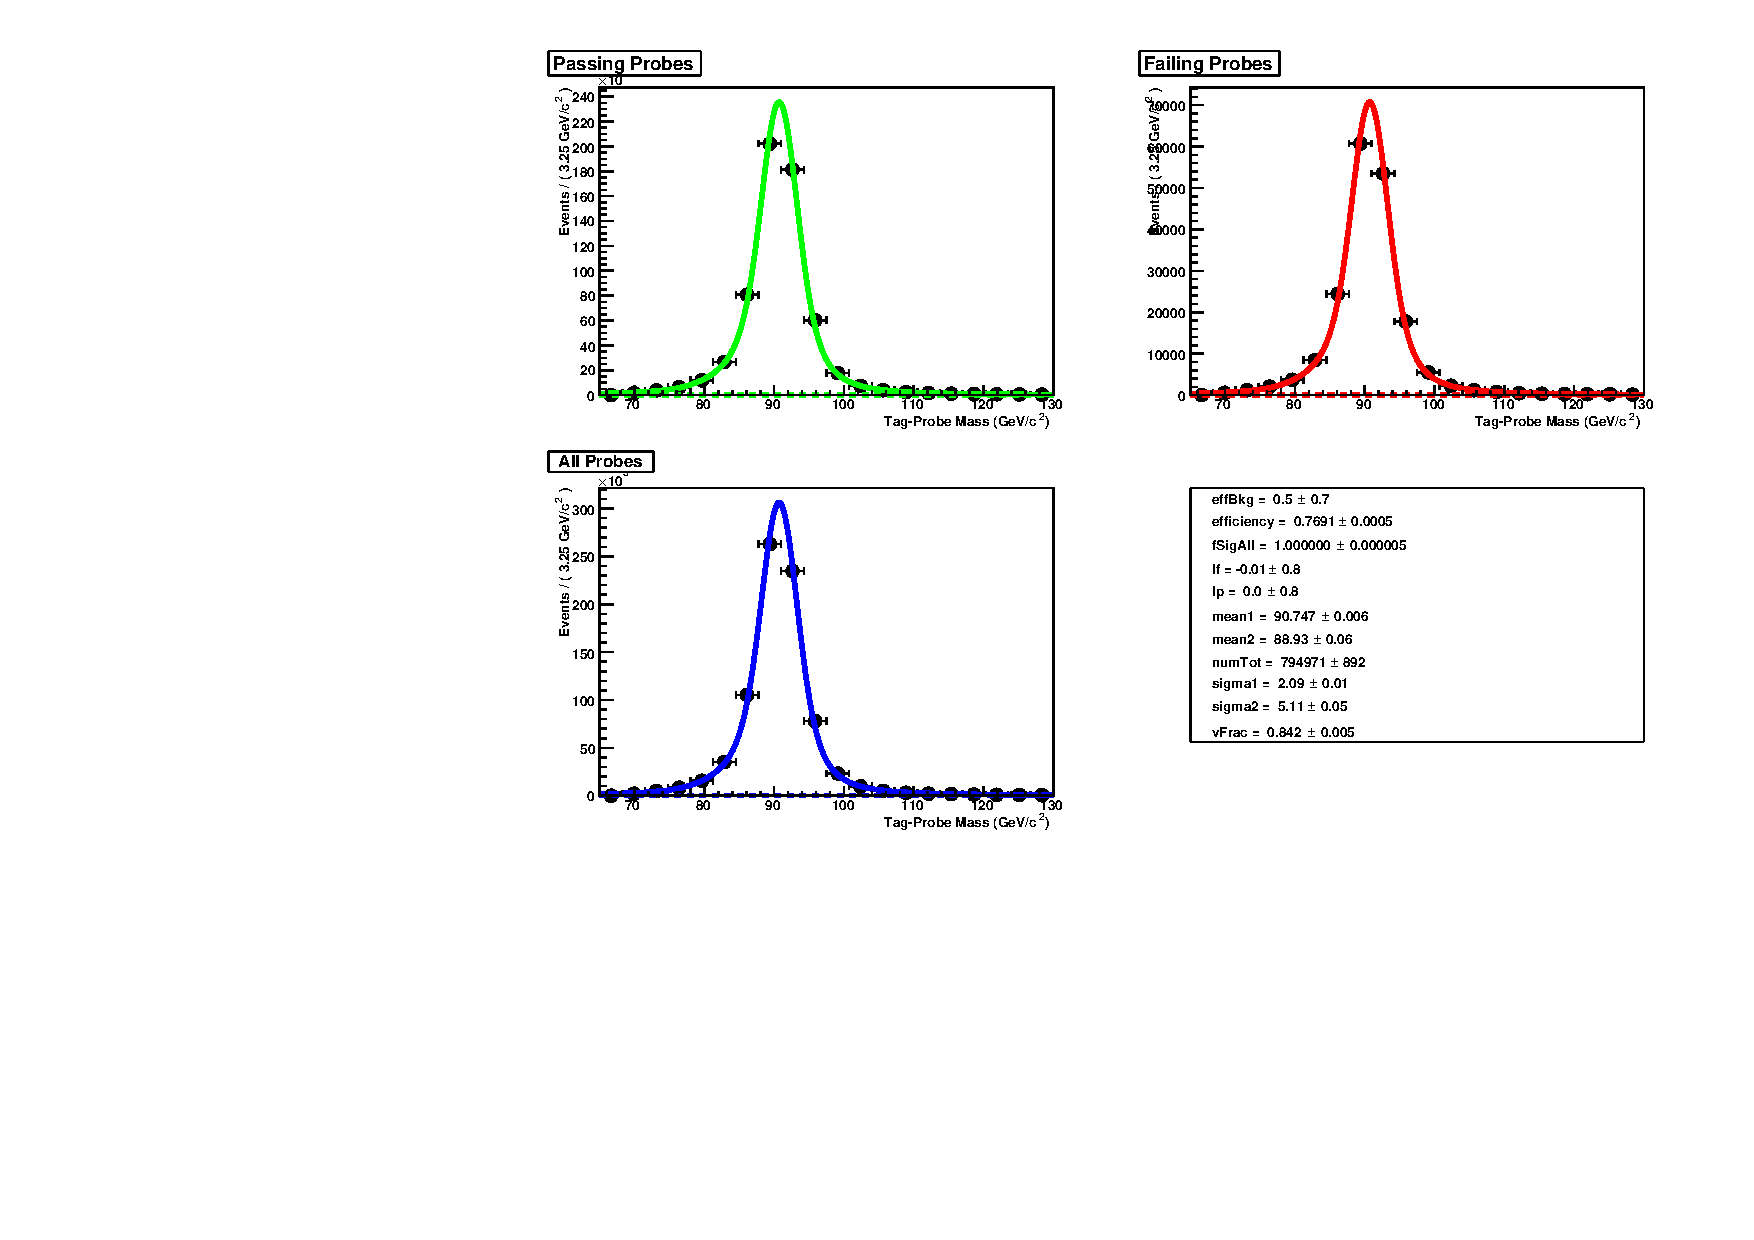
\includegraphics{Trigger/Figures/TaP/Mu23_data_fits}}
    \resizebox{0.48 \textwidth}{!}{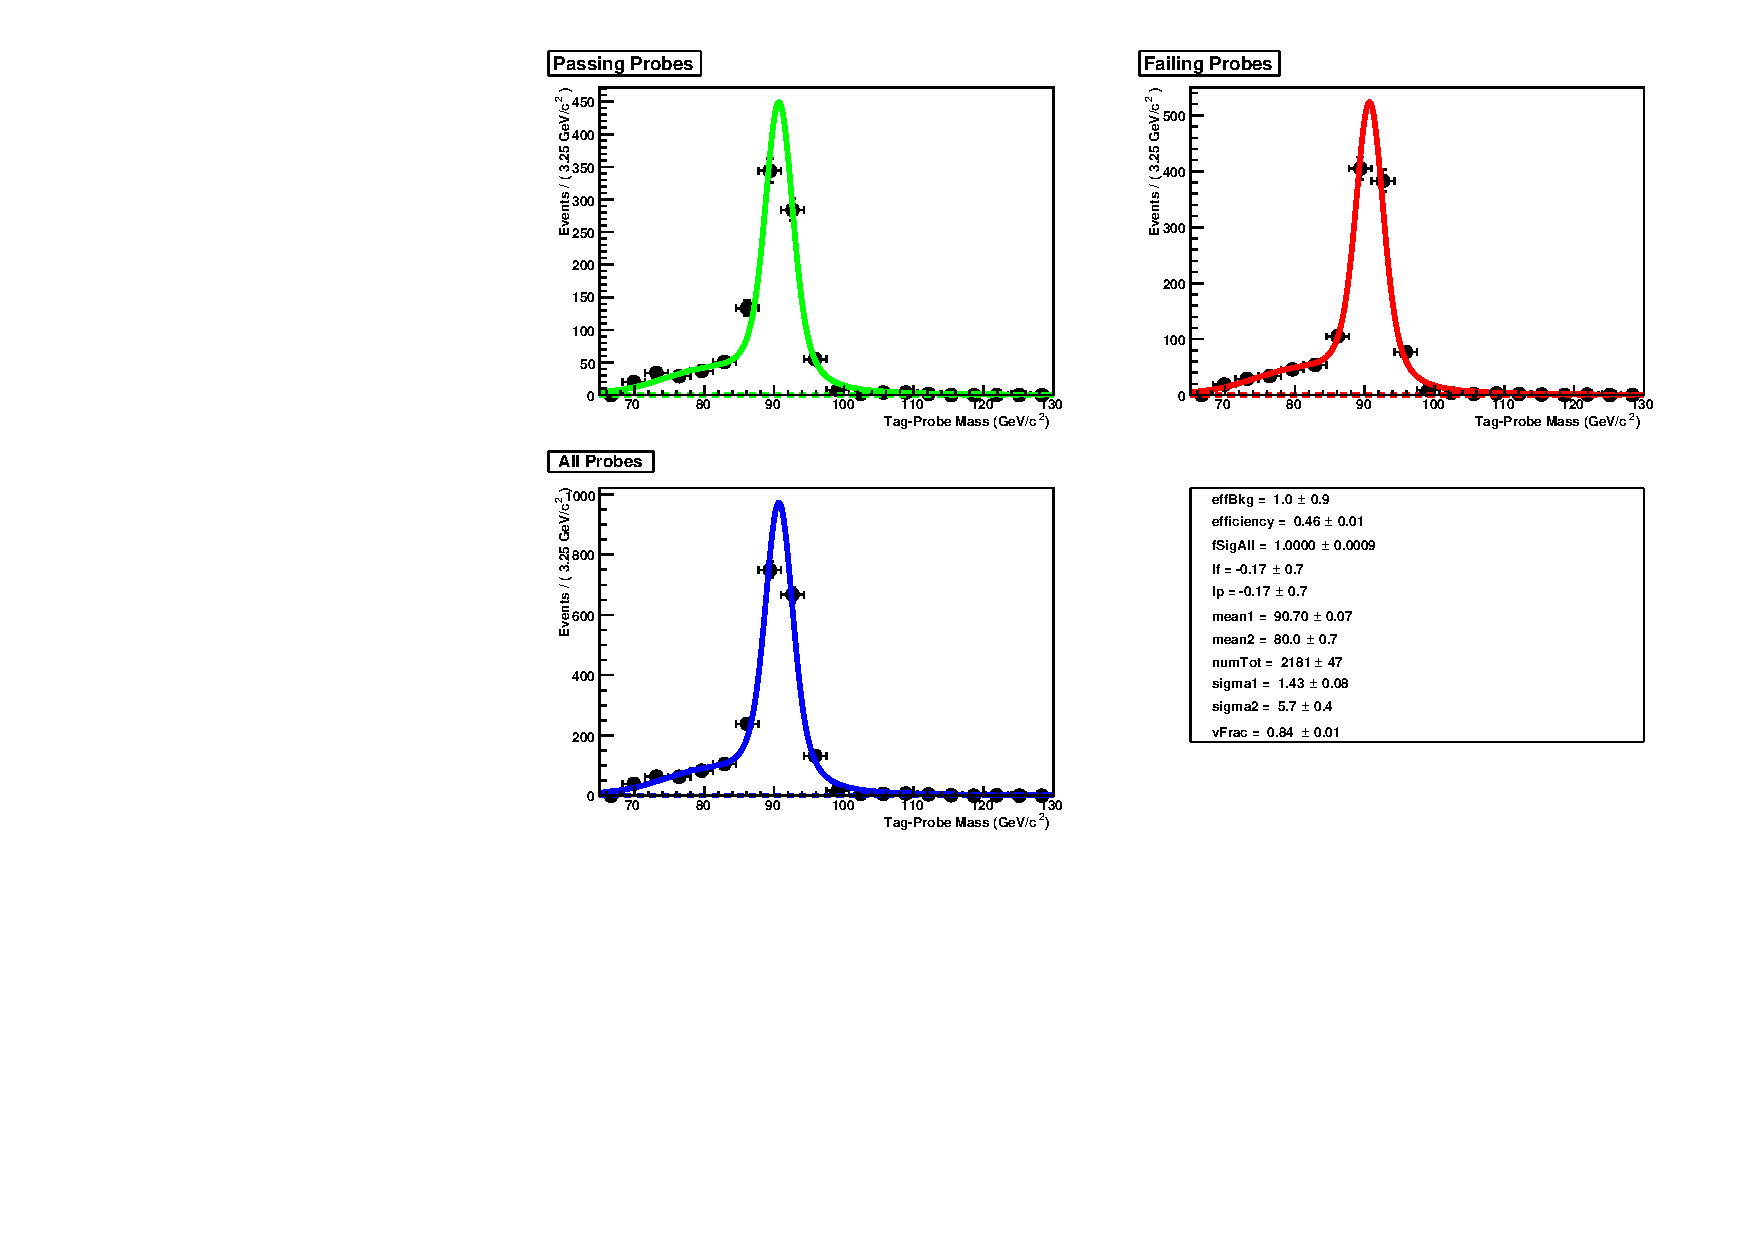
\includegraphics{Trigger/Figures/TaP/Mu23_MC_fits}}\\
    \resizebox{0.48 \textwidth}{!}{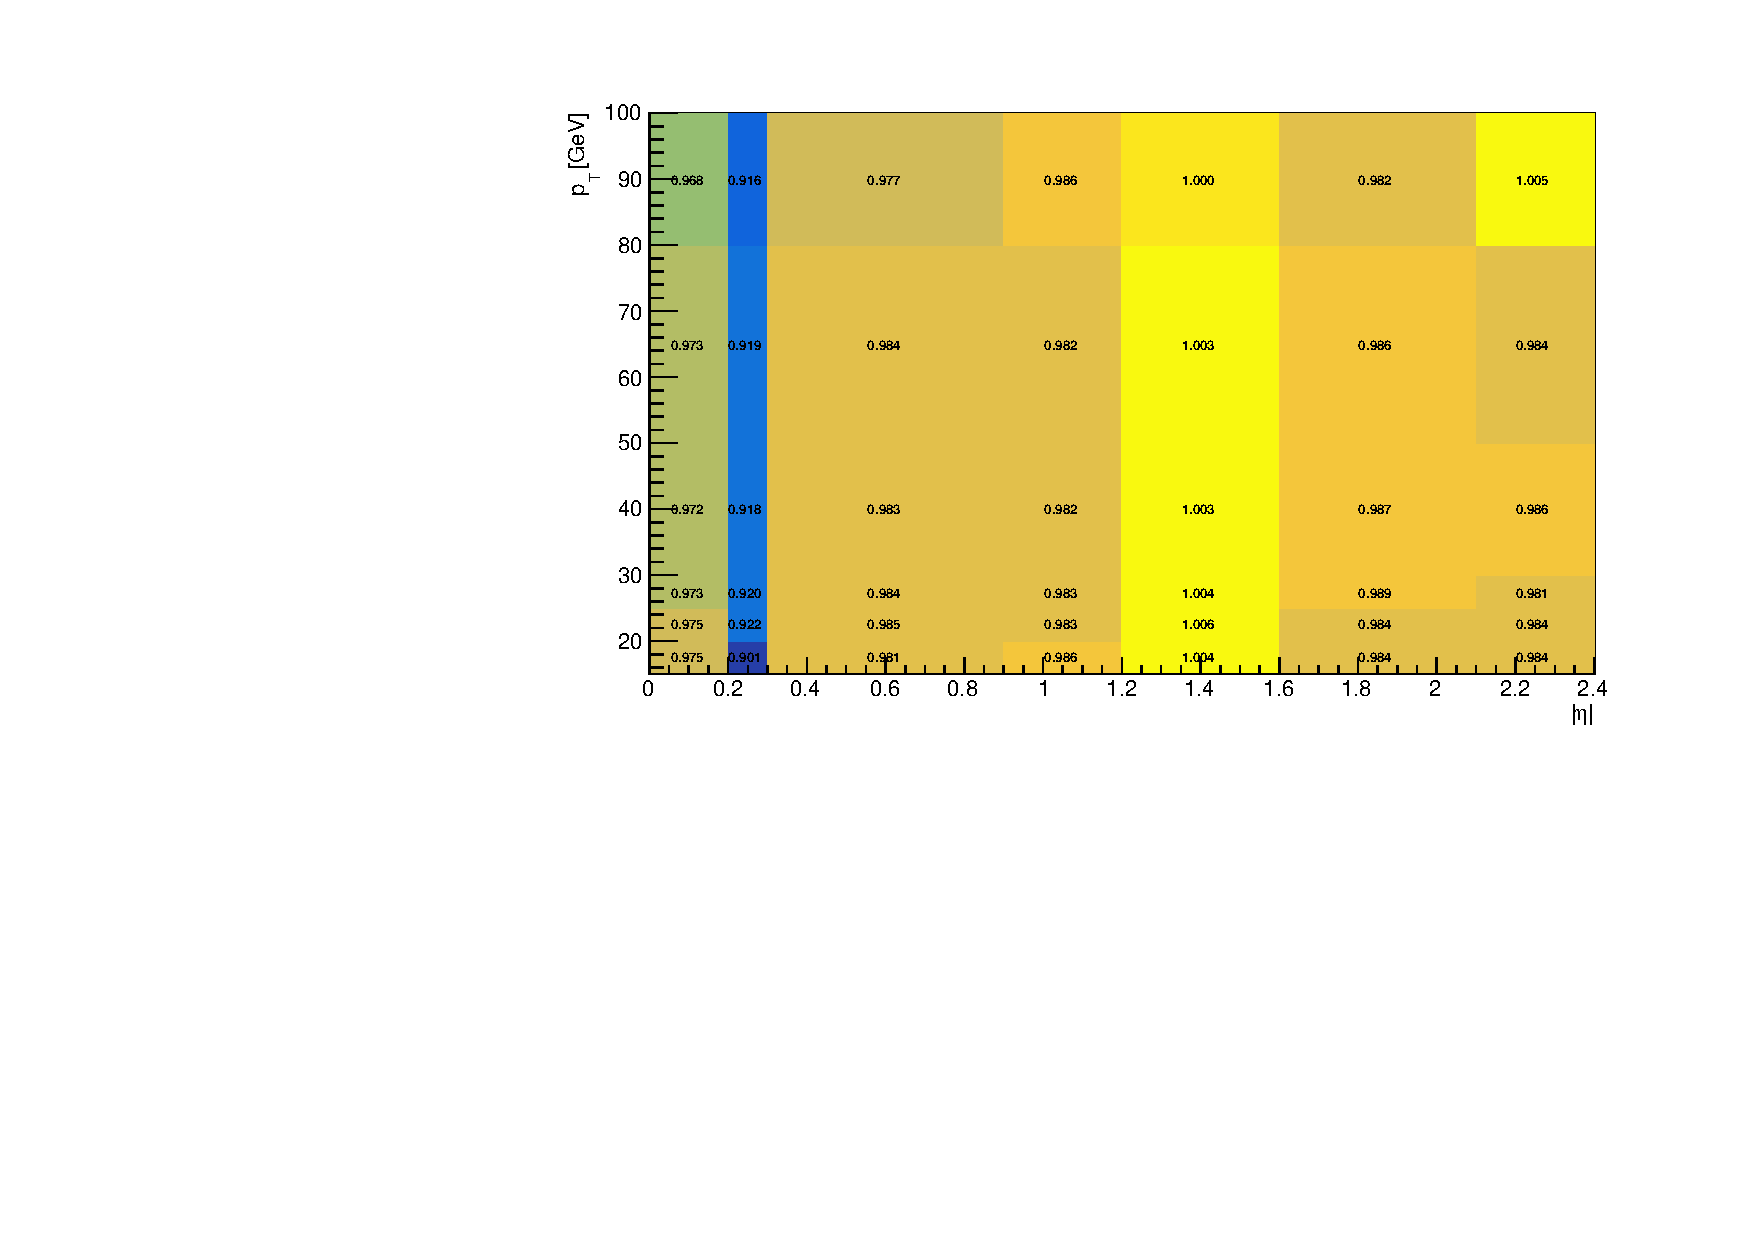
\includegraphics{Trigger/Figures/TaP/Mu23_sf}}
      \caption{Results of the trigger efficiency measurement with the Tag and Probe method for the Mu23 trigger leg. The upper row shows the measurement for one bin for each data (left) and simulation (right). The lower row shows 
       the scale factor between data and simulation binned in $\eta$ and \pt. }  
    \label{fig:TP_Mu23}
  \end{center}
\end{figure}

For the efficiency measurement the electron part ("electron leg") of the\\ HLT\_Mu8\_TrkIsoVVL\_Ele23\_CaloIdL\_TrackIdL\_IsoVL trigger for data and simulation and the corresponding scale factors sre shown in Figure \ref{fig:TP_Ele23}.
Here the efficiency on simulation is not determined with a fit, but by counting the events.

\begin{figure}[htbp!]
  \begin{center}
    \resizebox{0.6 \textwidth}{!}{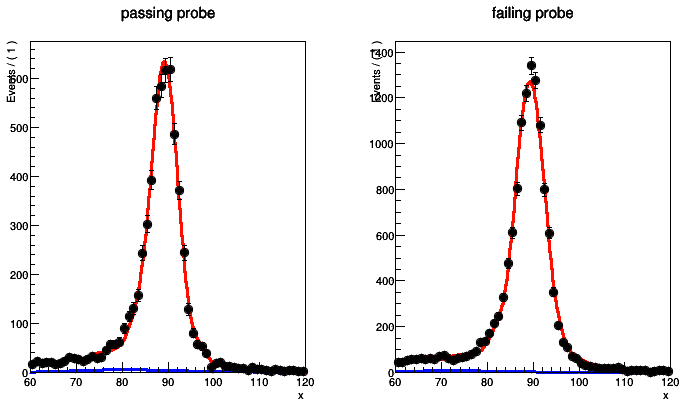
\includegraphics{Trigger/Figures/TaP/ele_plots_only}}
    \resizebox{0.39 \textwidth}{!}{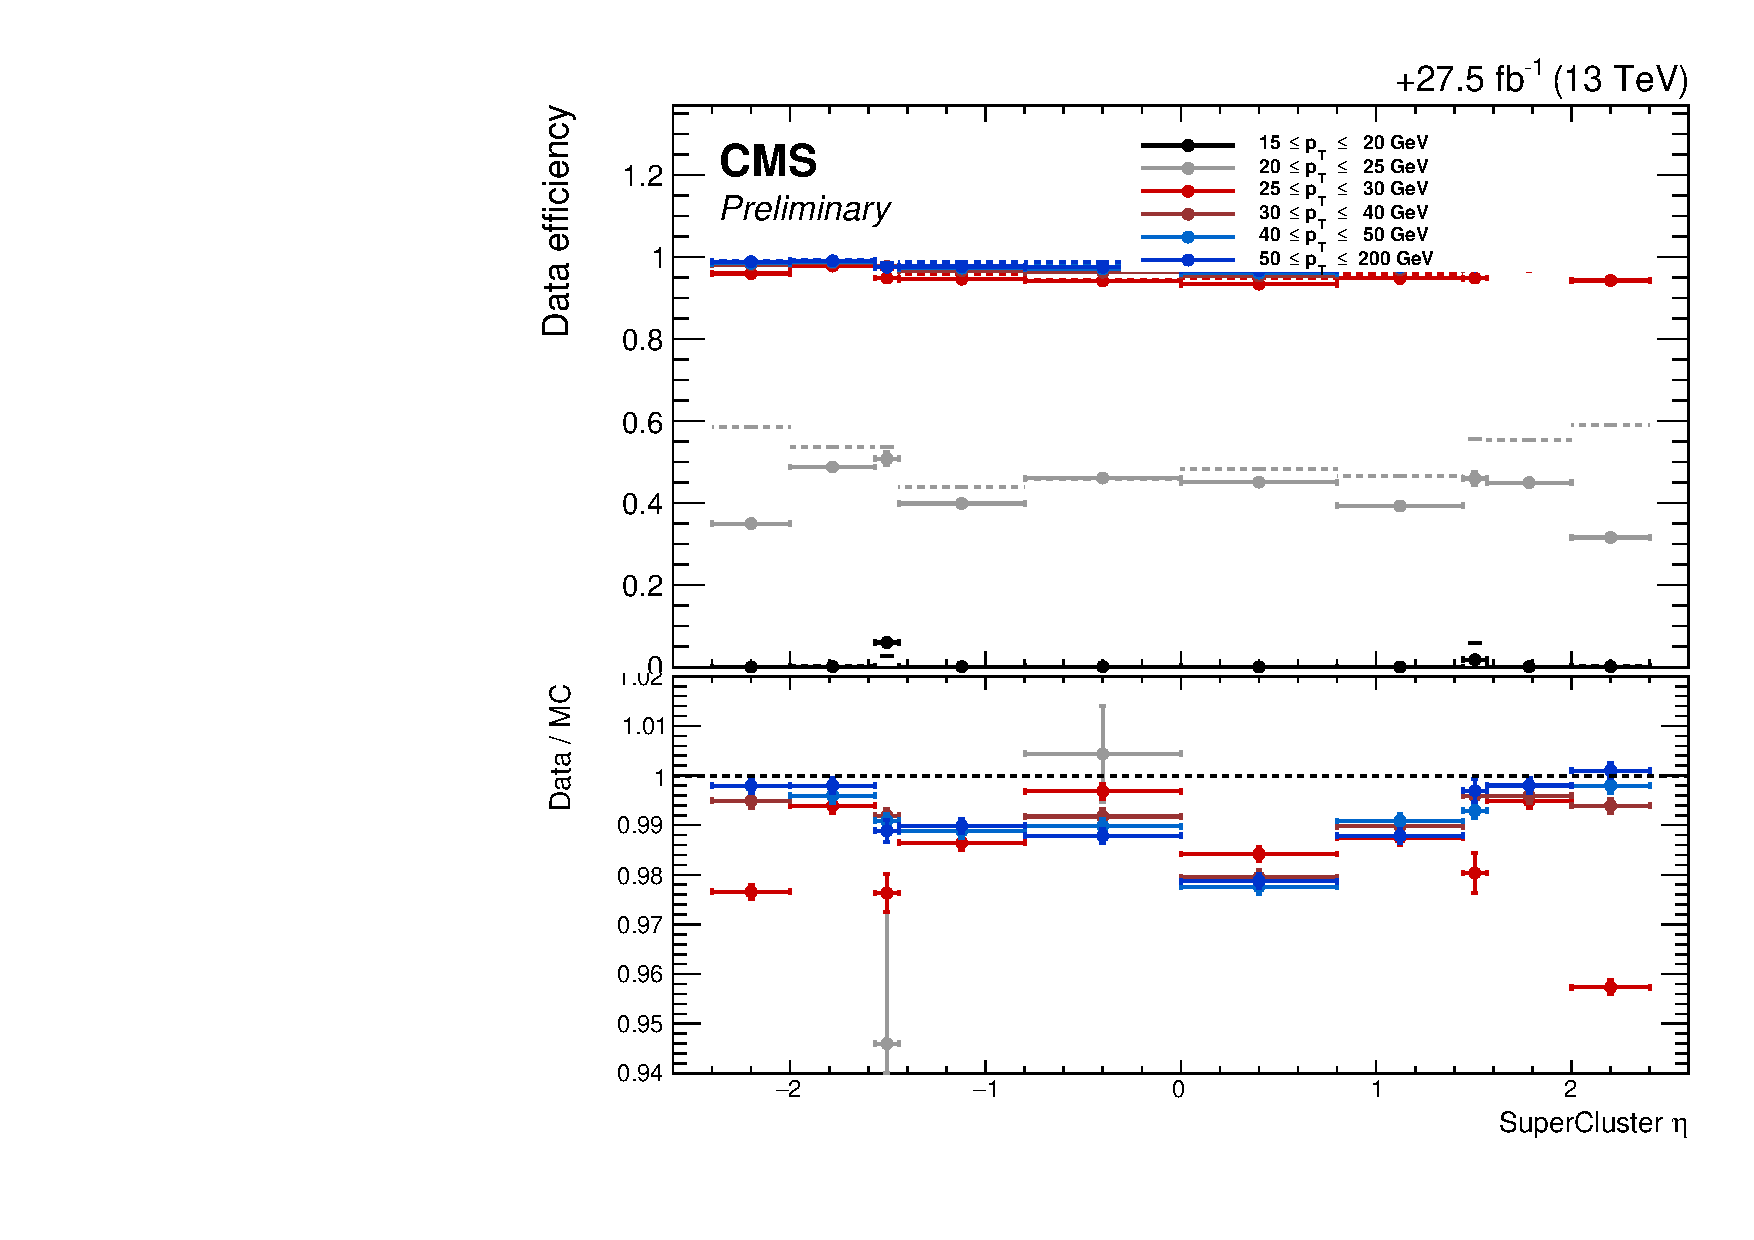
\includegraphics{Trigger/Figures/TaP/Ele23_data_eff}}
      \caption{Results of the trigger efficiency measurement with the Tag and Probe method for the Ele23 trigger leg. In the left plot the fit for one example bin in data is shown. The right plot shows the efficiency in data and simulation in bins of $\eta$ with multiple colored graphs showing the \pt dependence. Below that the scale factors are shown in the same format. }  
    \label{fig:TP_Ele23}
  \end{center}
\end{figure}


%********************************************** Fourth Section


\section{Comparison of Trigger Efficiency Measurements}
\label{sec:TriggerComp}

The two trigger efficiency measurements described in Sections \ref{sec:TriggerMetMethod} and \ref{sec:TriggerMetMethod} have one fundamental difference: The orthogonal trigger method measures the trigger efficiency for a complete trigger selection (multiple triggers) and per each event, which is mainly defined by the existence of two isolated leptons fullfilling some kinematic cuts. In contrast, the Tag and Probe method measures the trigger efficiency for each lepton of each trigger separately. 

These per leg efficiencies need to be combined to the efficiency for each di-lepton trigger. This is done by multiplying the efficiencies of the single trigger legs considering them to be uncorrelated. 
Then the efficiencies of each of the lepton triggers involved in the trigger selection needs to be combined. Since they are combined with a logical OR, this is done by multiplying the in-efficiencies of the trigger as in Equation \ref{eq:TPcombine}.

\begin{equation}
\varepsilon(trig_{combined}) = 1- (1-\varepsilon(trig_A))\cdot(1- \varepsilon(trig_B))
\label{eq:TPcombine}
\end{equation}

The combined trigger efficiency measured with the Tag and Probe method can be applied per event for the complete trigger selection. It can be then be compared to the trigger efficiency measured with the independent triggers.
For this comparison both efficiencies are applied to the same simulated \ttbar sample. These \ttbar events are required to contain an electron and a muon \textbf{TODO: reference to selection} and the trigger efficiency scale factors are applied depending on $\eta$ of these leptons.
After the rescaling, properties of these two sets of \ttbar events are compared as shown in Figure \ref{fig:Clos_emu}.

The distributions are consistent with each other in nearly the whole range of phase space. The largest disagreement is found for events with electrons with $\pt<20\GeV$, but these events are not considered for the final trigger efficiency scale factors. This agreement shows that there is no systematic difference between the two methods to measure a trigger efficiency in the \ttbar phase space. This does not necessarily apply to any other possible phase space, but the trigger efficiency measurement here specifically applies to the \ttbar phase space. This agreement is considered for the determination of the systematic uncertainties on the trigger efficiency.

\begin{figure}[htbp!]
  \begin{center}
    \resizebox{0.48 \textwidth}{!}{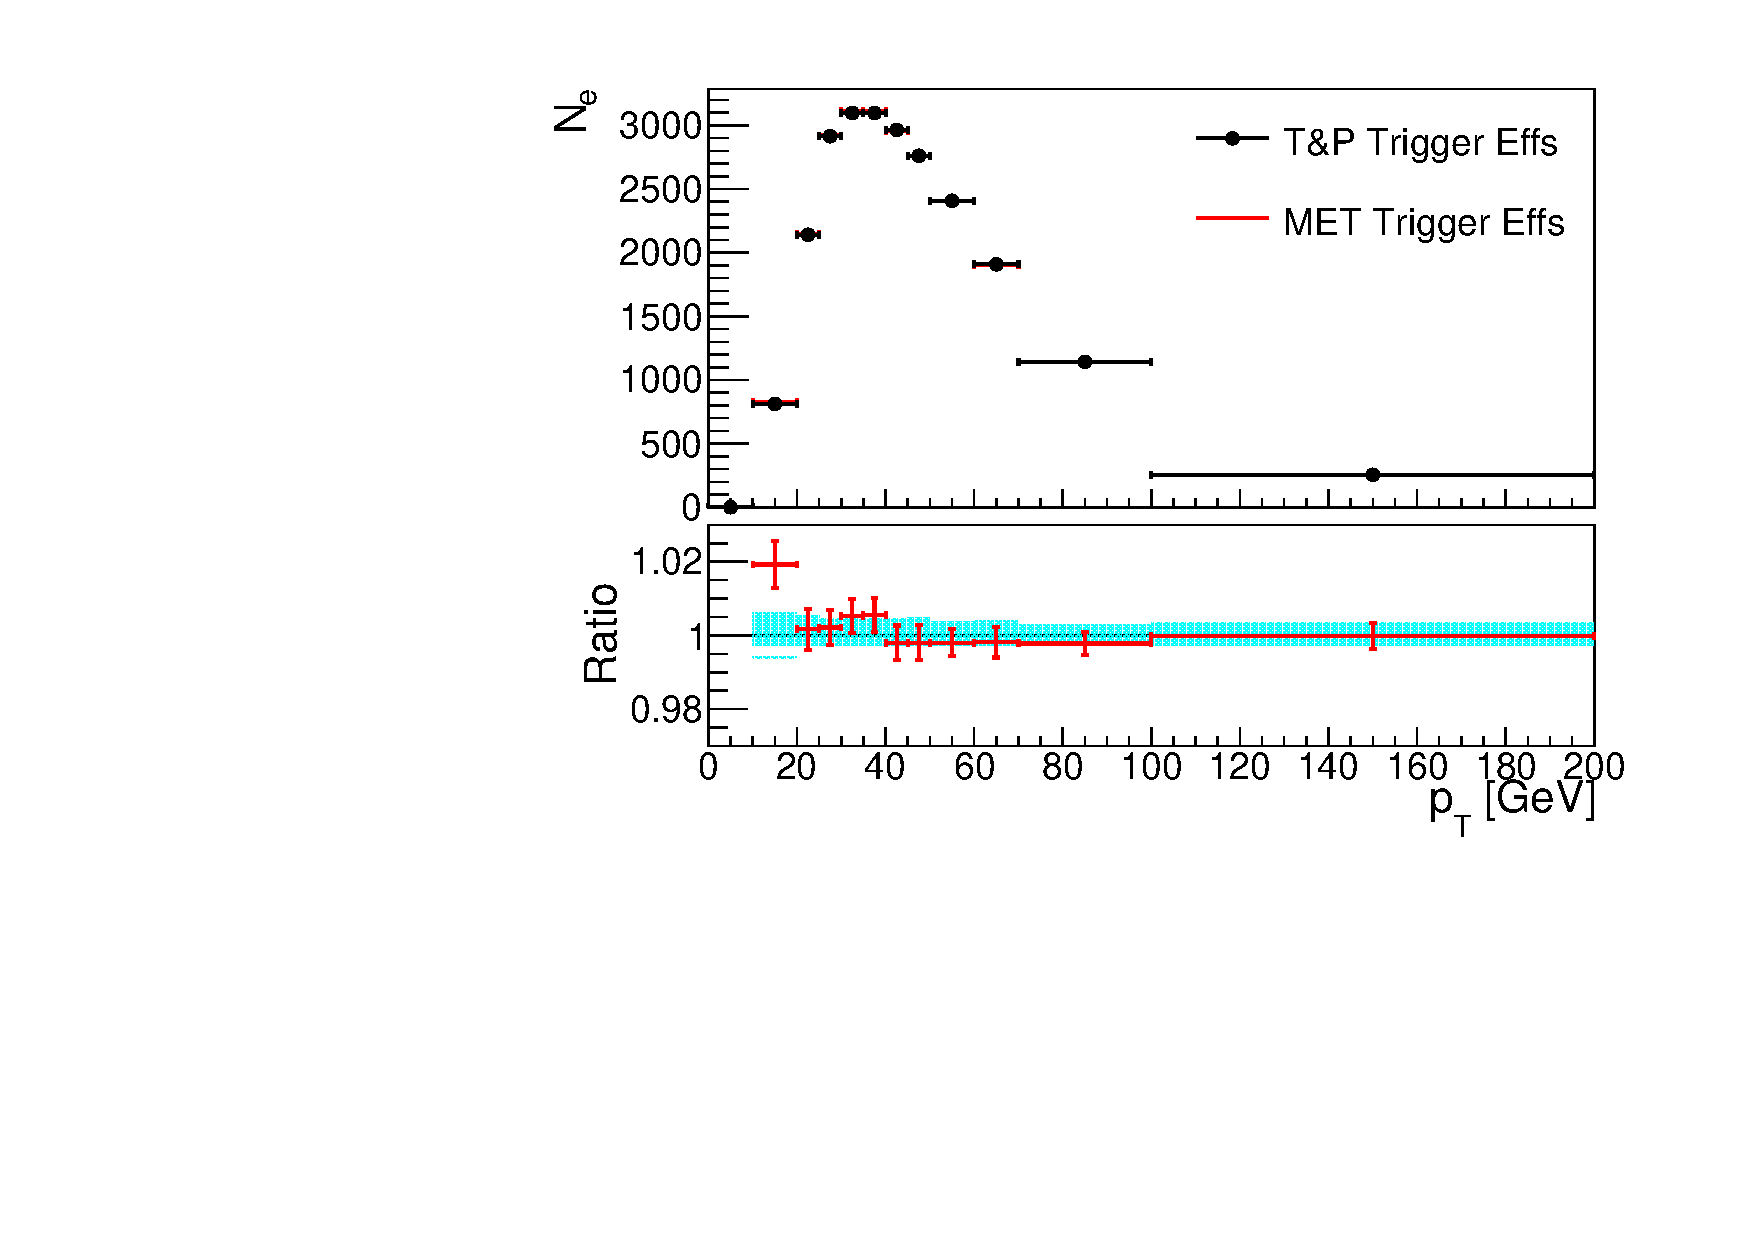
\includegraphics{Trigger/Figures/Clos/emu_ptele}}
    \resizebox{0.48 \textwidth}{!}{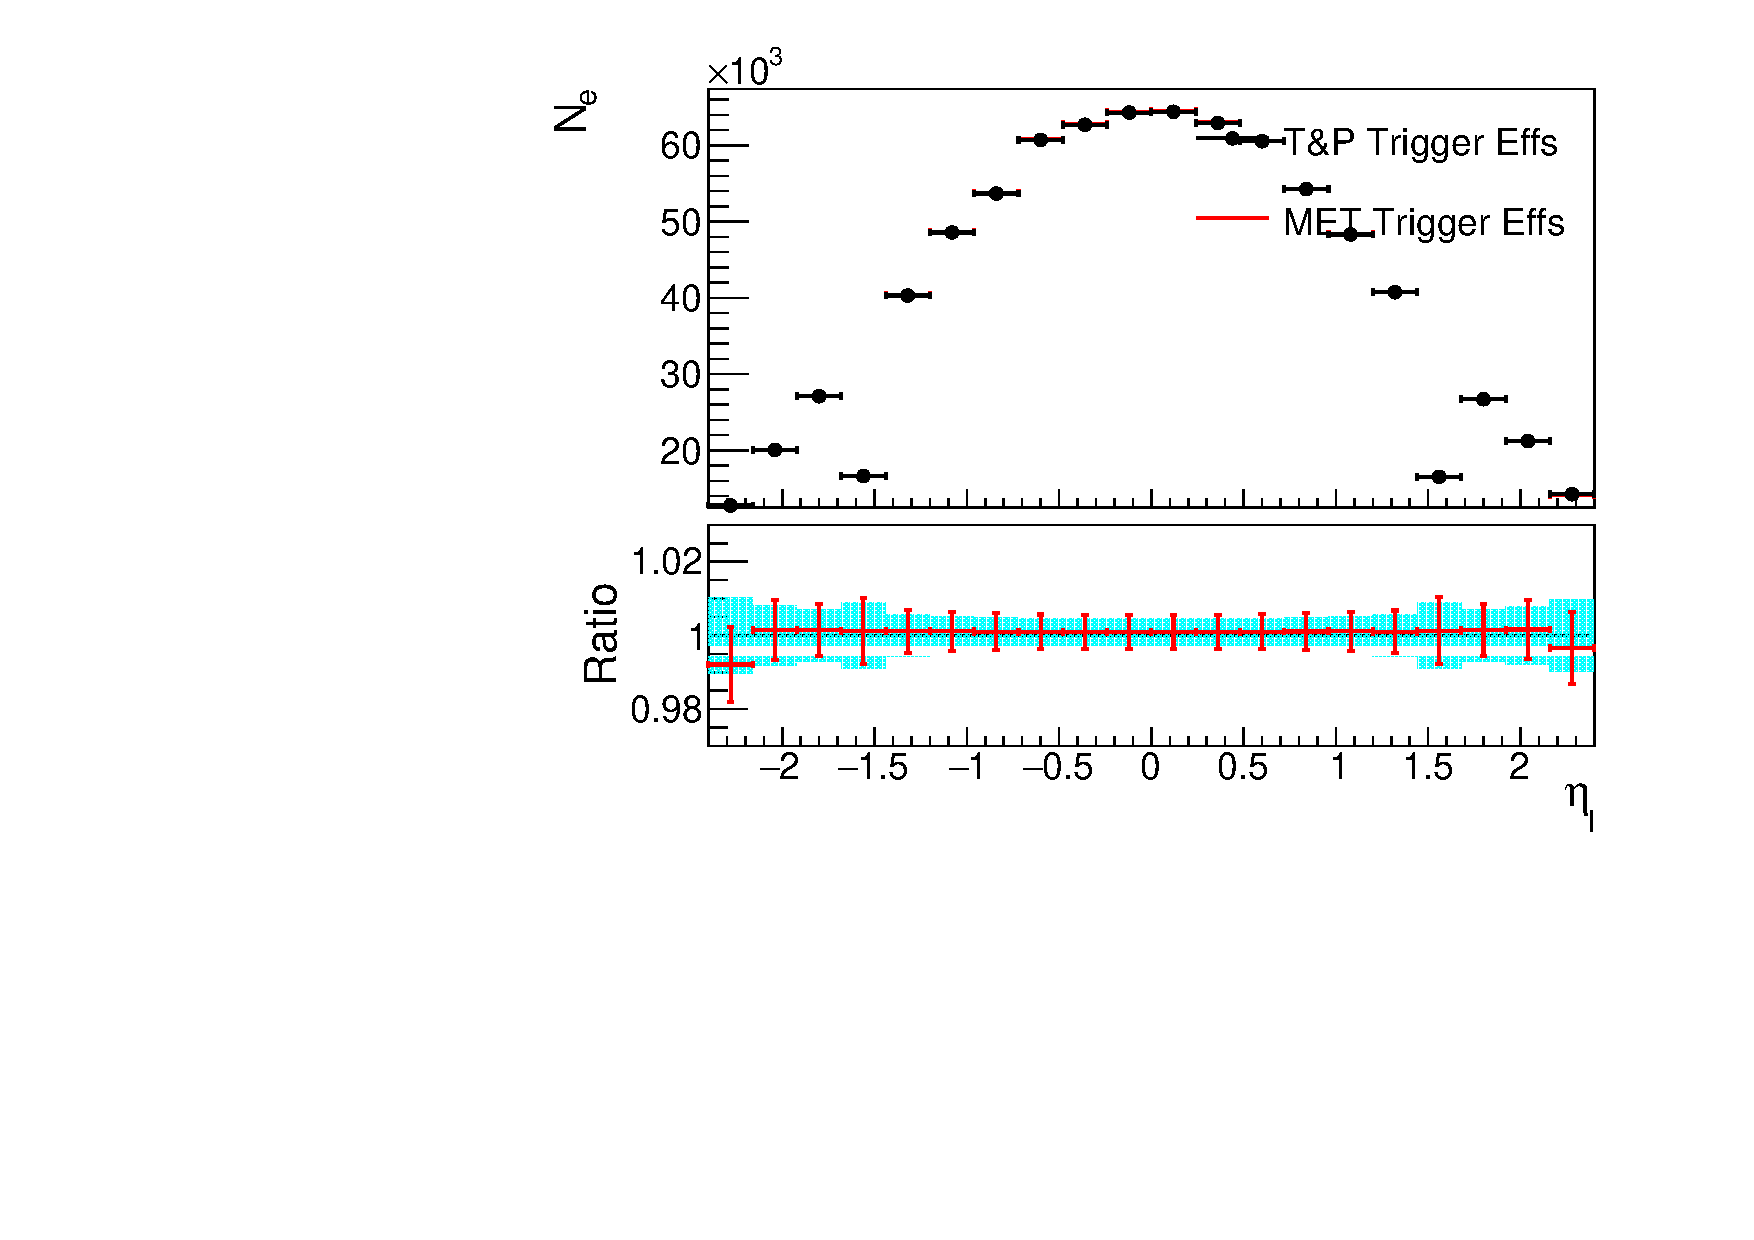
\includegraphics{Trigger/Figures/Clos/emu_etaele}}\\
    \resizebox{0.48 \textwidth}{!}{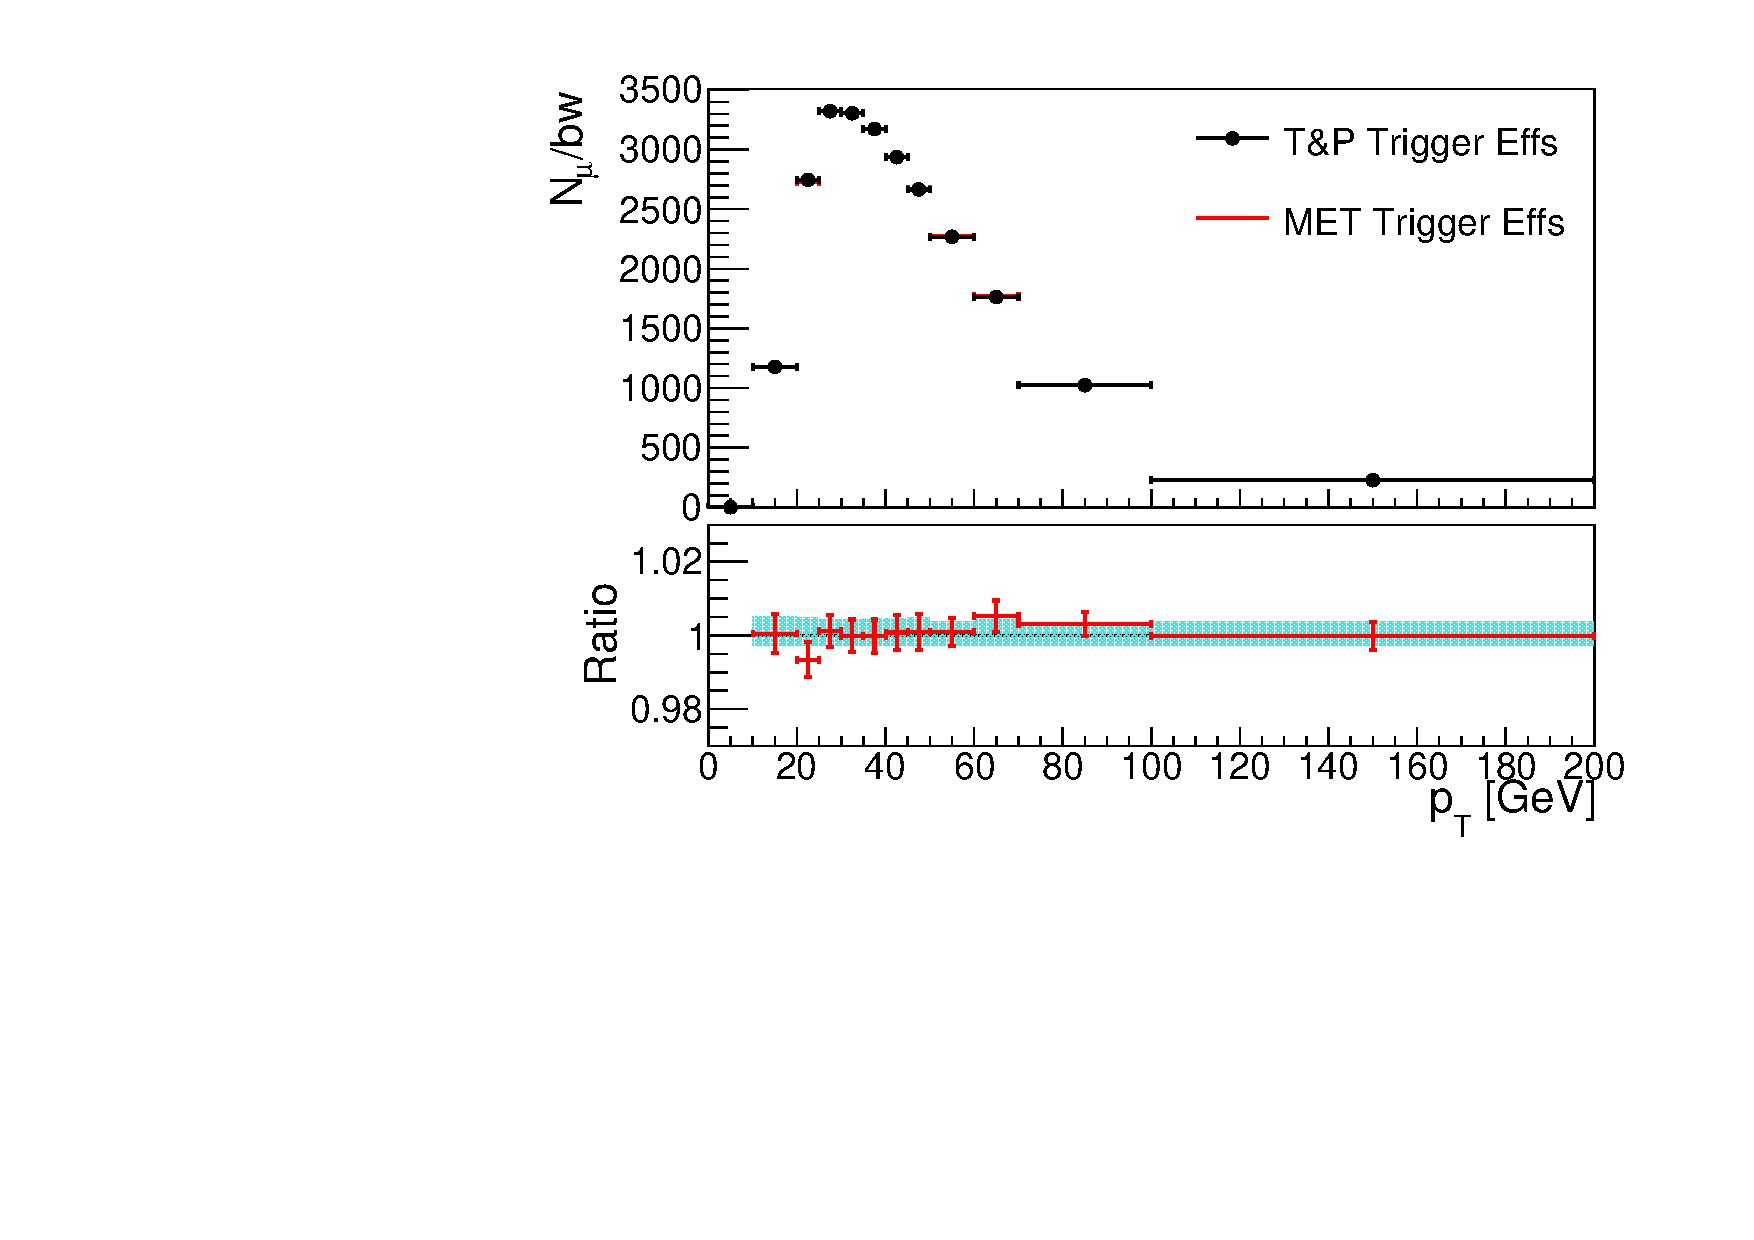
\includegraphics{Trigger/Figures/Clos/emu_ptmu}}
    \resizebox{0.48 \textwidth}{!}{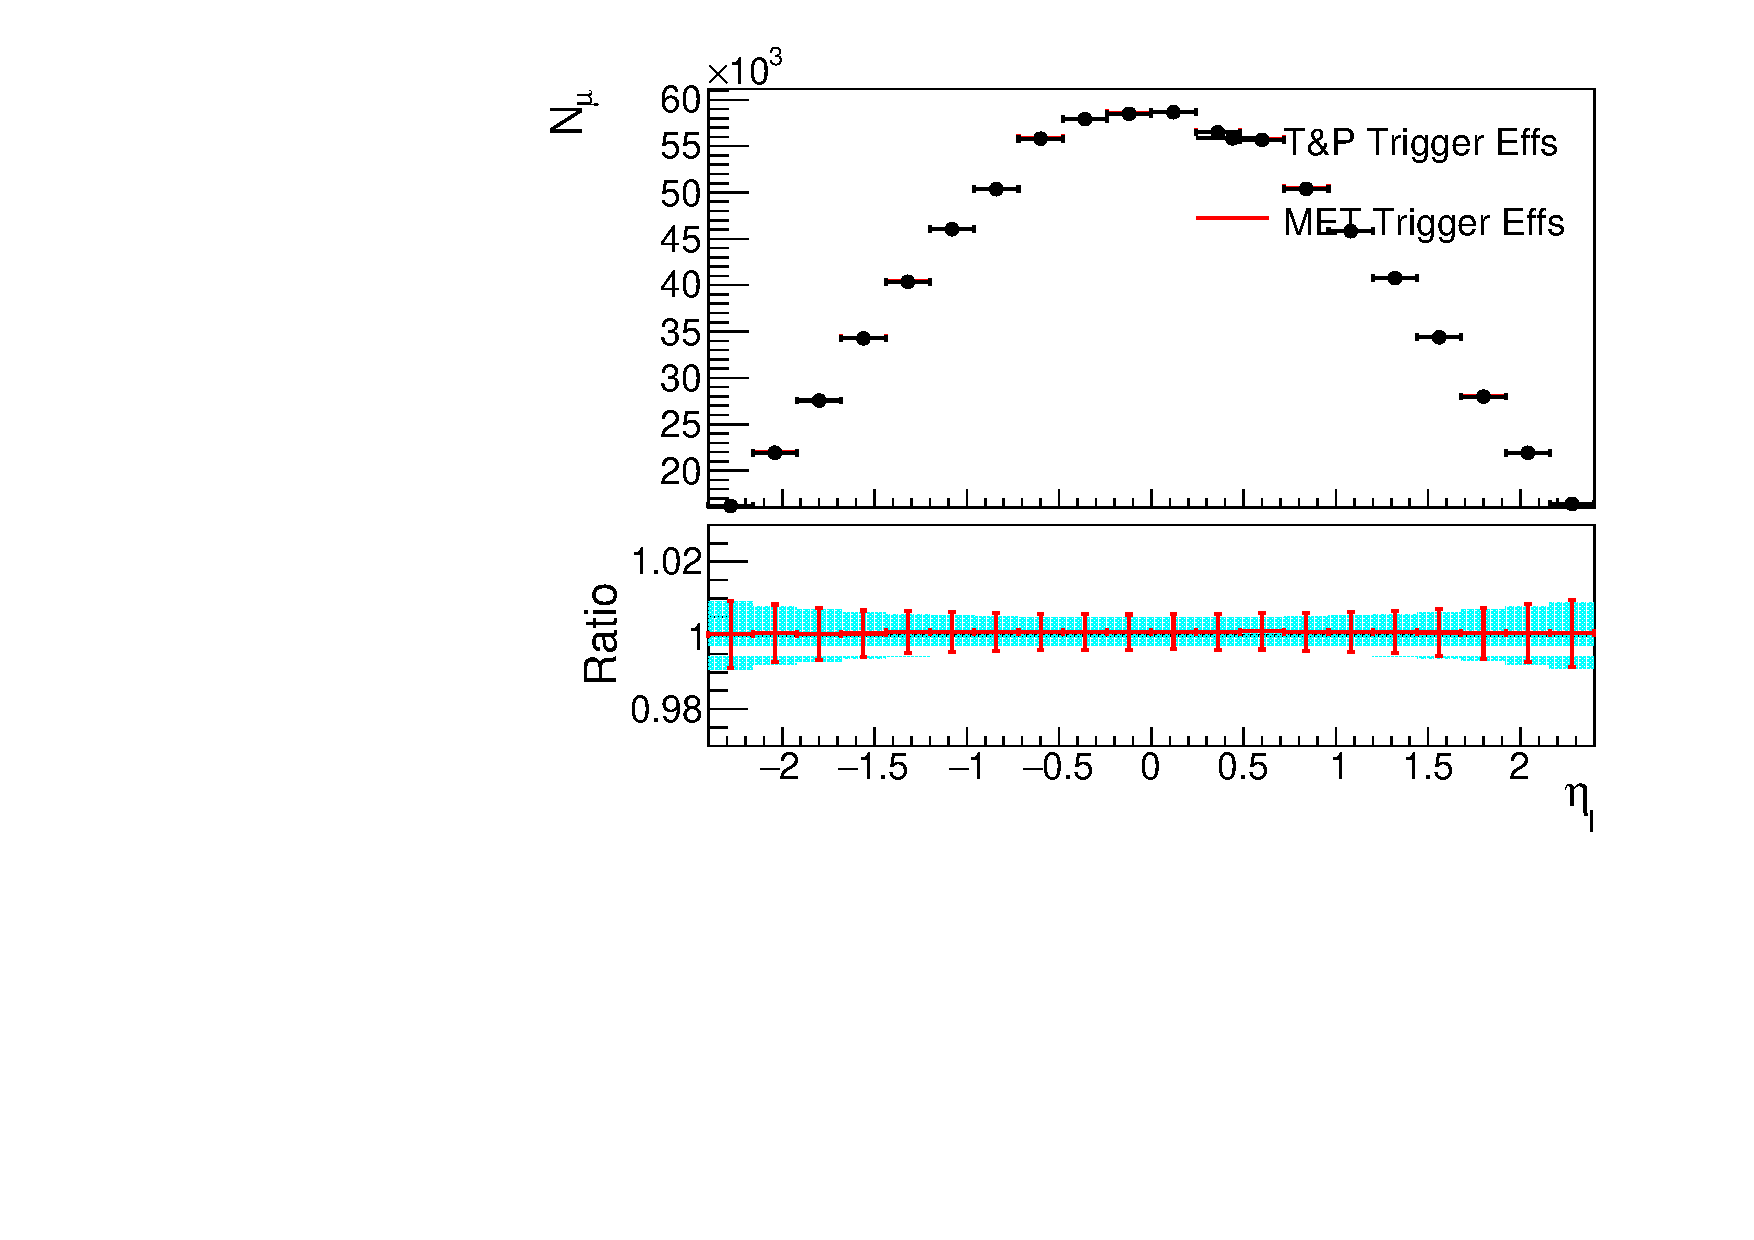
\includegraphics{Trigger/Figures/Clos/emu_etamu}} \\
    \resizebox{0.48 \textwidth}{!}{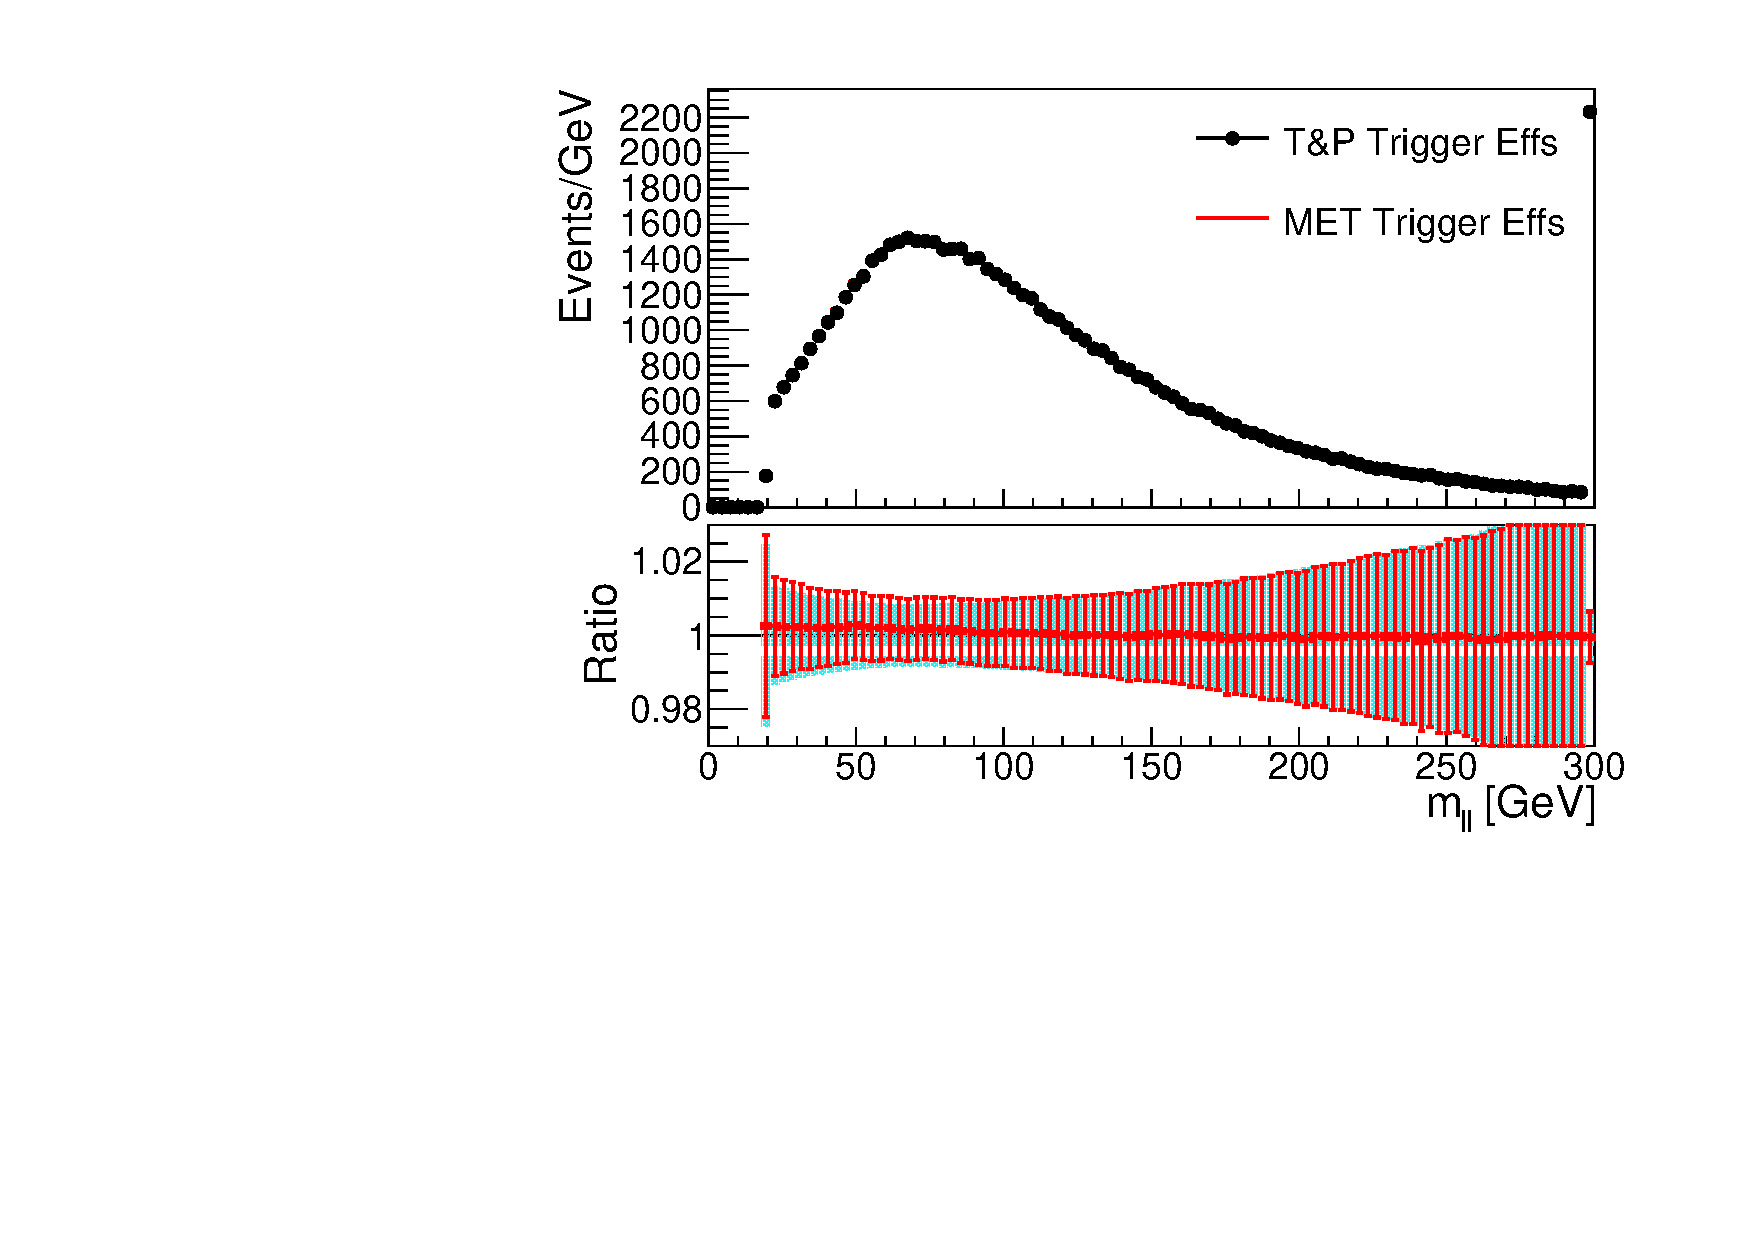
\includegraphics{Trigger/Figures/Clos/emu_mll}}
    \resizebox{0.48 \textwidth}{!}{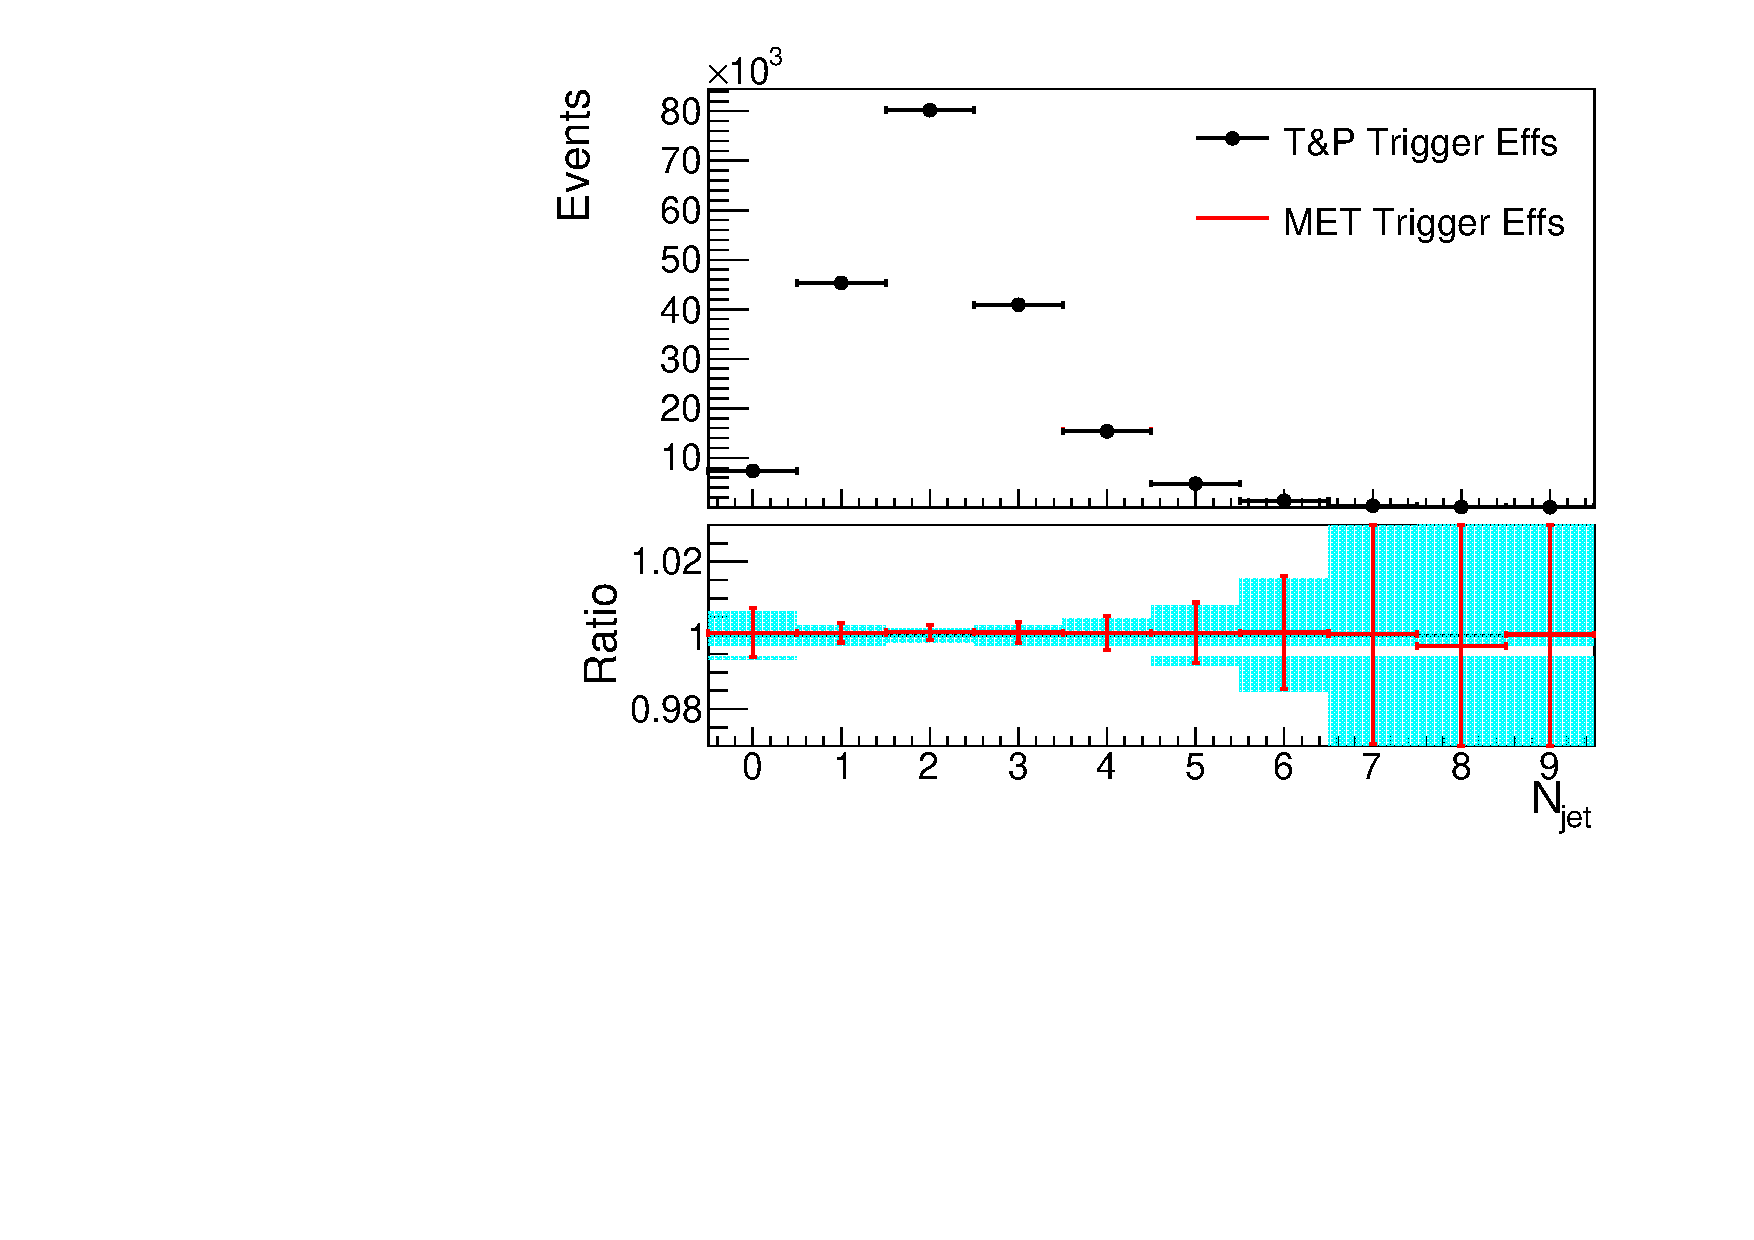
\includegraphics{Trigger/Figures/Clos/emu_njets}}        
      \caption{Comparison of \ttbar simulation reweighted according to the trigger efficiencies measured with the Tag and Probe method and with independent \ETm triggers.
       The top row shows the comparison in bins of \pt (left) and $\eta$ (right) of the electron. The middle row shows it in bins of \pt (left) and $\eta$ (right) of the muon. The bottom row shows it in bins of the invariant mass of the dilepton system(left) and the number of jets (right). The uncertainties shown are statistical. The lower panels show the ratio of the distribution reweighted with the efficiency from the \ETm trigger method divided by the distribution reweighted by the Tag and Probe method. }  
    \label{fig:Clos_emu}
  \end{center}
\end{figure}

\section{Determination of the Trigger Scale Factor}

\label{sec:TrigSF}

The factor correcting the trigger efficiency in simulation to the data is determined using the independent trigger method described in Section \ref{sec:TriggerMetMethod}. 
As it measures the trigger efficiency directly per event for the complete trigger selection and does not require any additional assumptions on the correlations between the triggers or the respective parts of the triggers it is prefered to the Tag and Probe method. 

Based on the comparison of the two methods (see Section \ref{sec:TriggerComp}), a remaining systematic uncertainty of $0.3\;\%$ is applied in addition to the statistical uncertainty.
Systematic and statistic uncertainty are added up in quadrature. 

The scale factors are binned in $|\eta|$ of the two leptons. This provides a good compromise between covering disagreements between data and simulation seen in Section \ref{sec:TriggerMetMethod} and sufficient statistical power for each bin.

These scale factors are shown in Figure \ref{fig:TrigSF} .

\begin{figure}[htbp!]
  \begin{center}
    \resizebox{0.48 \textwidth}{!}{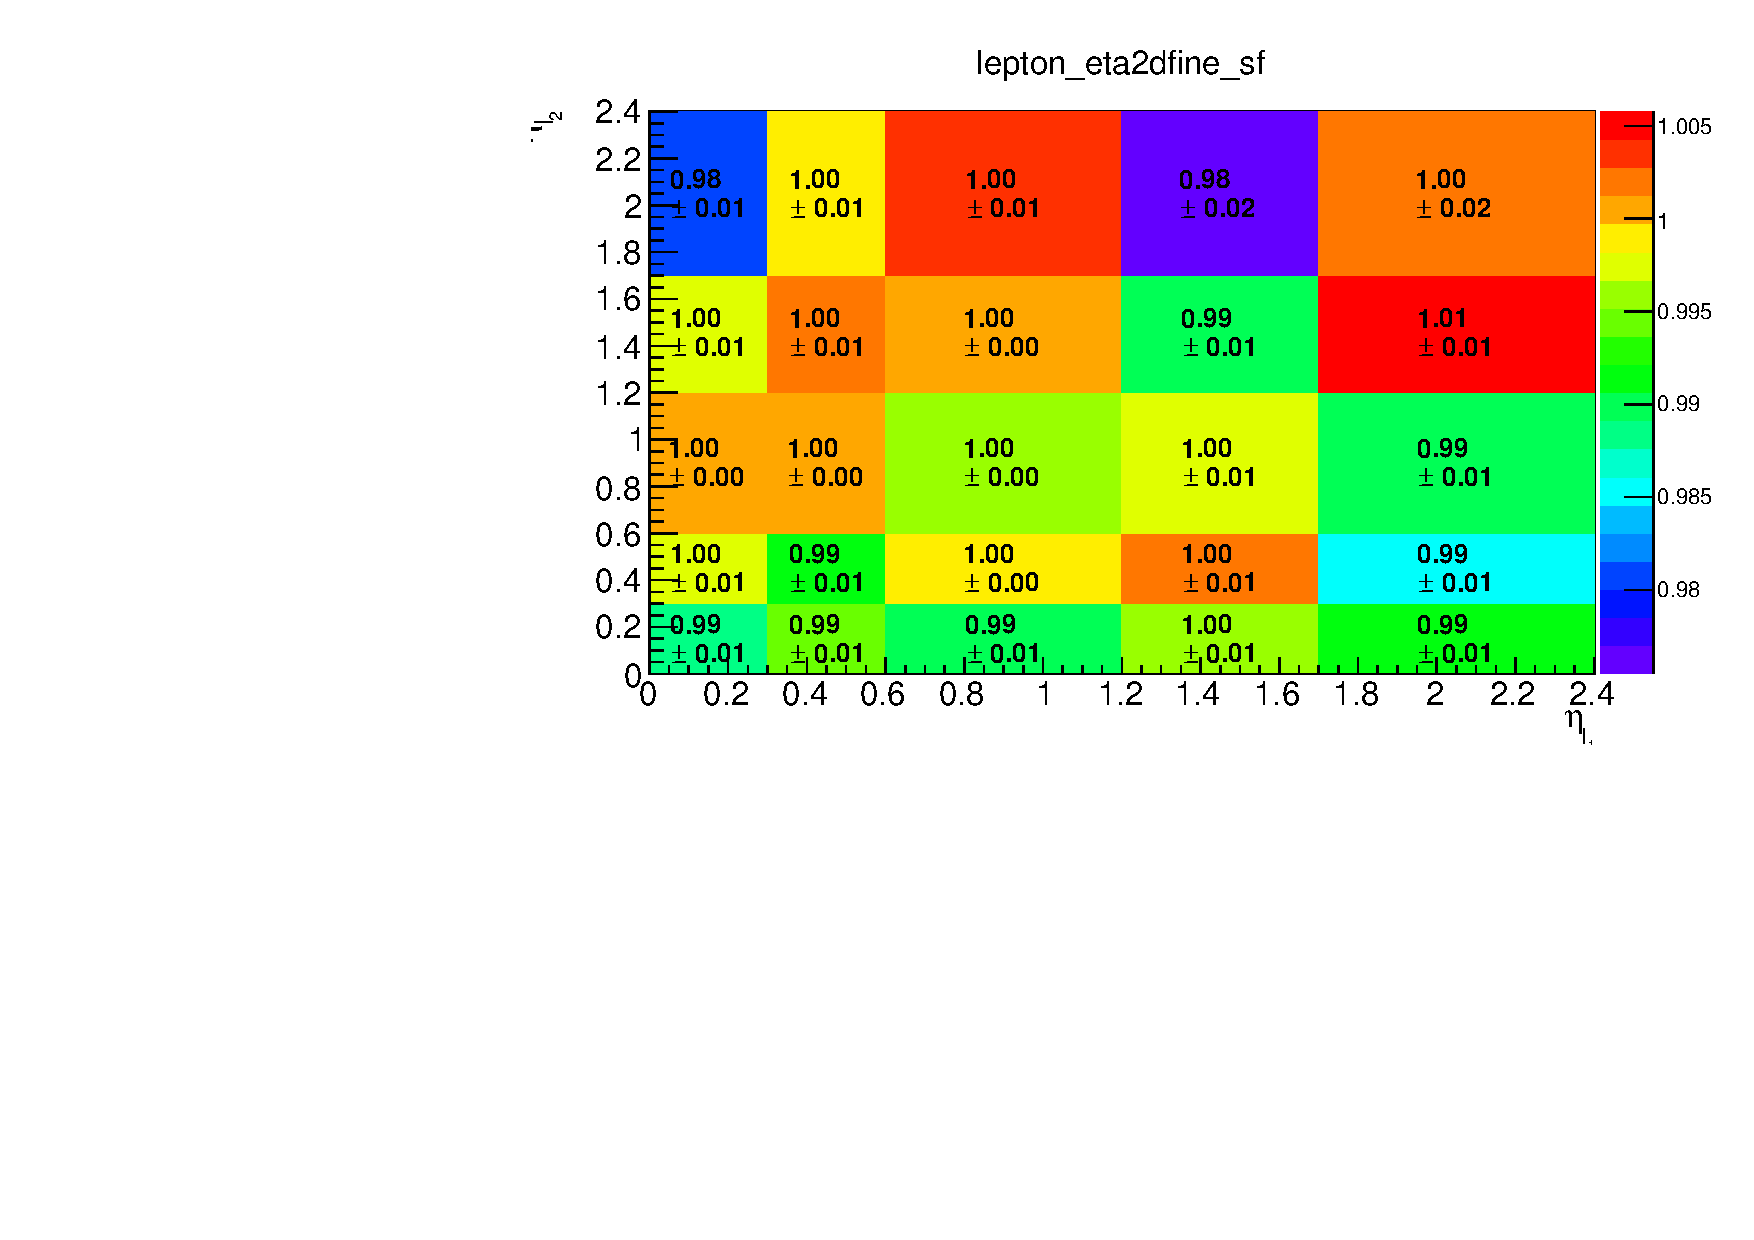
\includegraphics{Trigger/Figures/emu_eta2d_sf}}
    \resizebox{0.48 \textwidth}{!}{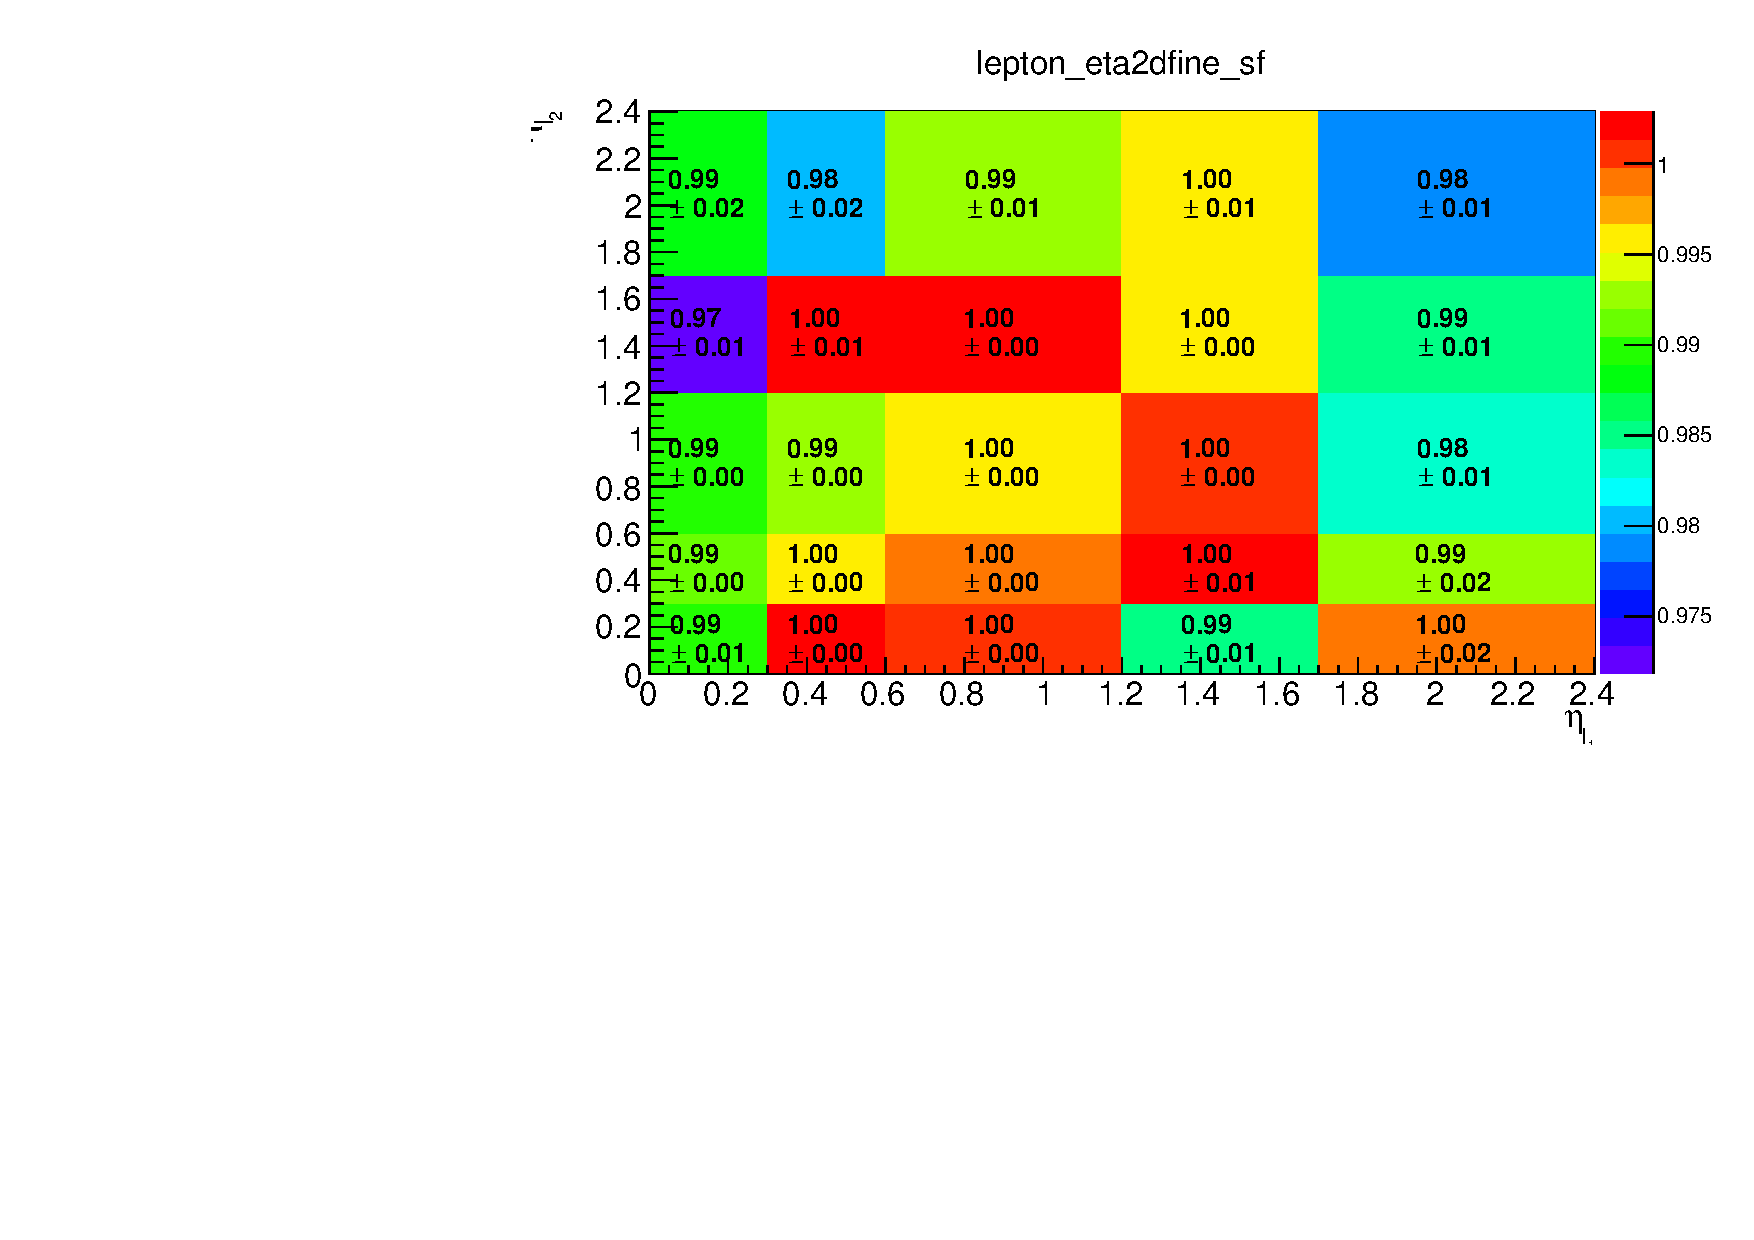
\includegraphics{Trigger/Figures/mumu_eta2d_sf}}\\
    \resizebox{0.48 \textwidth}{!}{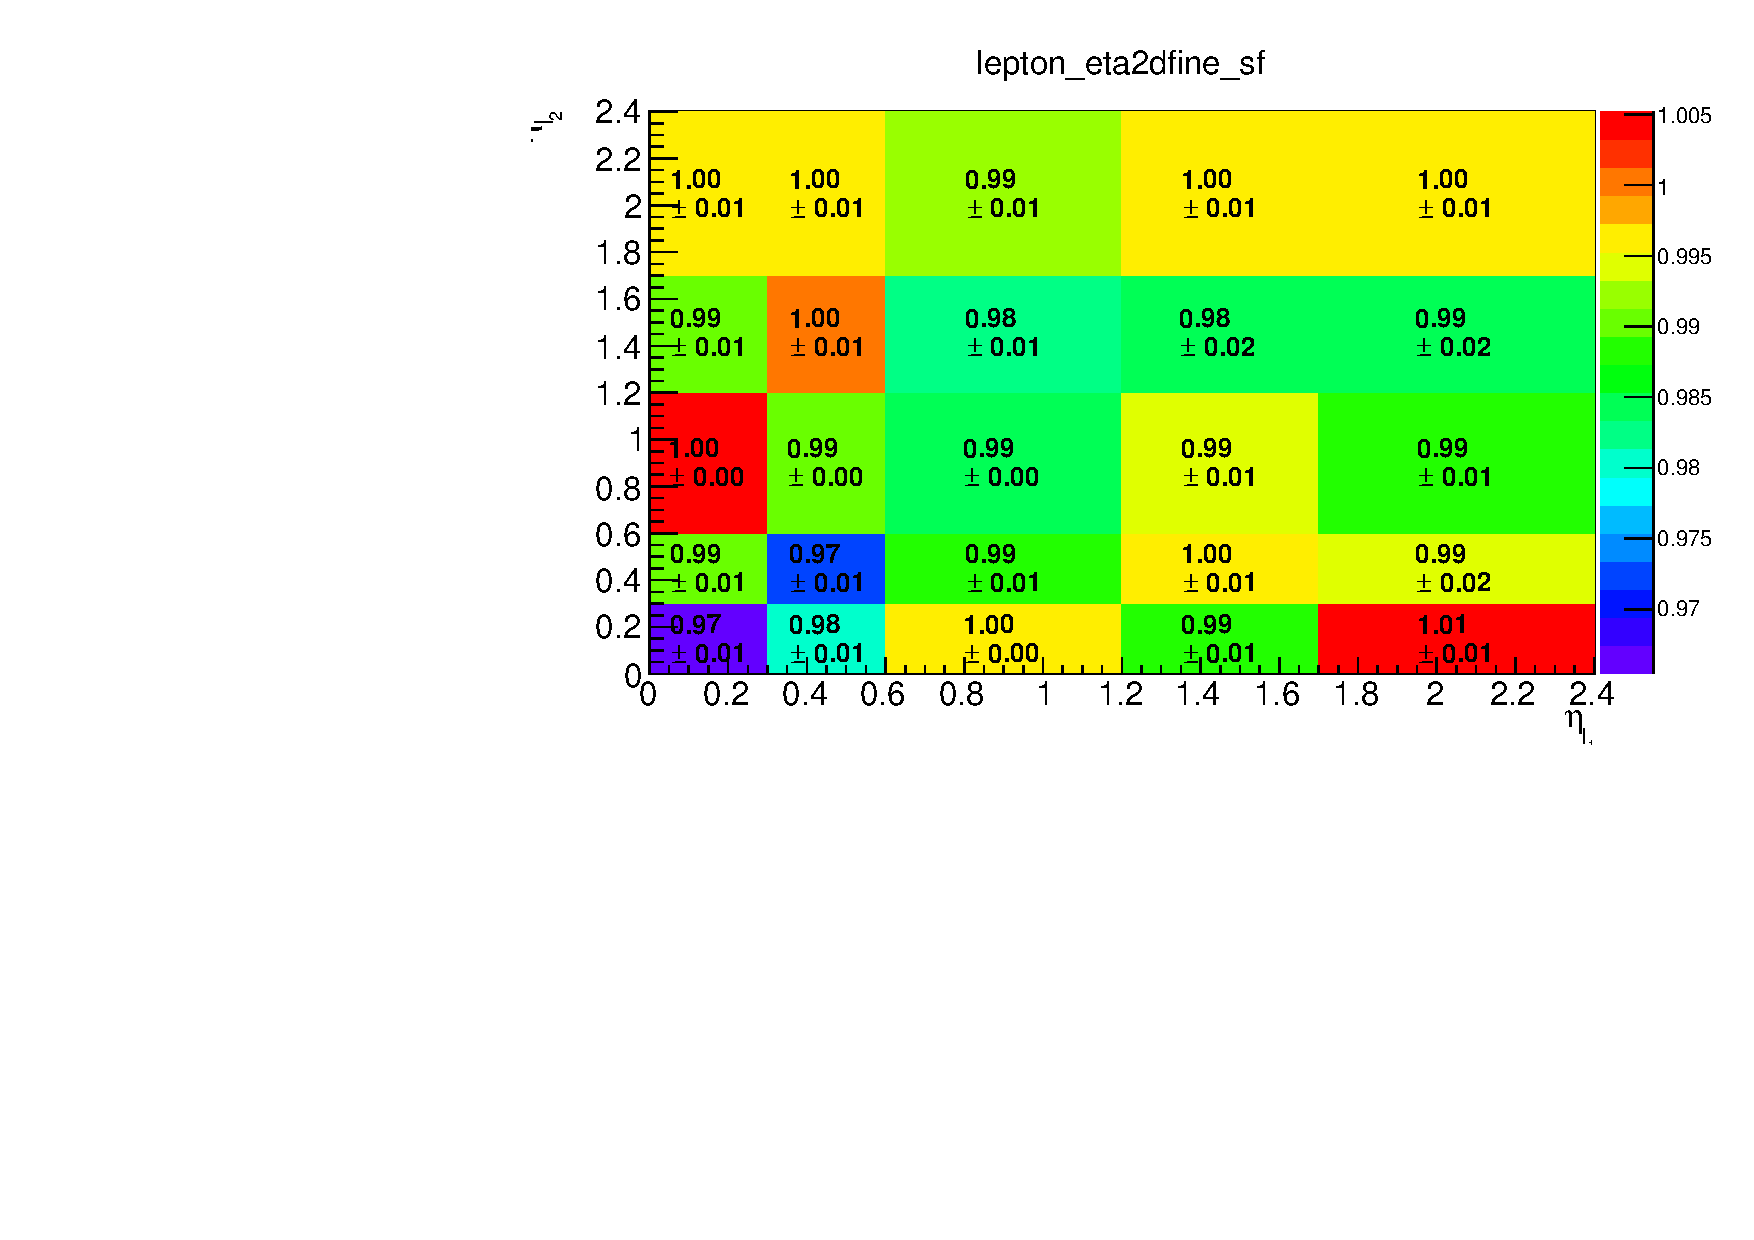
\includegraphics{Trigger/Figures/ee_eta2d_sf}}       
      \caption{Scale factors from the trigger efficiencies of the trigger selection in the \emu (top left), \mumu (top right) and \ee (middle) channel. The scale factors are given in bins of the $|\eta|$ of the two leptons. The errors denote the combination of statistical and systematic uncertainties.}  
    \label{fig:TrigSF}
  \end{center}
\end{figure}








%!TEX root = ../thesis.tex
%*******************************************************************************
%****************************** Third Chapter **********************************
%*******************************************************************************
\chapter{Measurement of the Top Quark Pair Production Cross Section}

The measurement of the top quark production cross section requires multiple steps.
First, the events that are to be used in the measurement need to be selected as described in Section \ref{sec:xsec_sel}.
Based on this selection the simulation is compared to data to assure that the simulation gives a good estimation of the actual measurement (see Section \ref{sec:xsec_datamc}).
On that dataset the cross section is then measured using a template based binned $\chi^2$ fit as described in Section \ref{sec:xsec_fit}.
The templates are chosen to maximize the precision of the analysis as described in Section \ref{sec:xsec_templates}.
Then the fitting procedure and the statistics model are described in more detail in Section \ref{sec:xsec_stat}.
Finally the extrapolation from the full to the fiducial cross section is discussed in Section \ref{sec:xsec_extraction}.

In general the cross section can be measured according to Equation \ref{eq:CaC}. Here $N_{top}$ denotes the number of selected events containing a top quark pair, $A$ denotes the acceptance of the selection,
$\varepsilon$ denotes the efficiency of the selection and $\mathcal{L}$ denotes the luminosity.

\begin{equation}
\sttbar = \frac{N_{top}}{A \cdot \varepsilon \cdot \mathcal{L}}
\label{eq:CaC}
\end{equation} 

Since the selected sample does not only contain top quark pair events the amount of background needs to be determined.
This is done here by fitting template predictions for all relevant background processes and \ttbar to the data.

\section{Event Selection}
\label{sec:xsec_sel}

The aim of the selection is to select a dataset that is dominated by \ttbar events.
At the same time it also defines acceptance and with it the visual phase space, which should be as broad as possible.
This can partially be solved by using different cuts in the different lepton decay channels and then relying on the principle
of lepton universality in the extrapolation.

All events need to fullfill the trigger selection described in detail in Section \ref{sec:Triggersel}.

In the dilepton channel events need two isolated and well defined leptons \todo{Link to reconstruction chapter}.
Both leptons also need to be within the coverage of the tracker fullfilling the condition of $|\eta| < 2.4$.
For electrons the gap region of the electronic calorimeter $1.4442<|\eta|<1.566$ is vetoed as well.
The decay is then defined according to the two leptons leading in \pt requiring the leading lepton to have $\pt > 25 \GeV$
and the sub leading lepton to have $\pt > 20 \GeV$. 
According to these two leptons the events are then classified into the \emu,\ee and \mumu channels.

The mass of the dilepton system is required to have $\mll > 20 \GeV$ to avoid contamination from low mass DY events.
In the same-flavor channels the window of the Z-mass resonance is vetoed $76 \GeV < \mll <106 \GeV$ to reduce the dominant background of 
resonant Drell-Yan production.

Jets are required to have $\pt > 30 \GeV$ and $|\eta|<2.4$. In order to identify b-tagged jets a tight working point is chosed, giving as high 
purity for selected b-tagged jets.

In the same flavor channels events are required to contain one b-tagged jets, while in the \emu channel does not include any requirement on the jets.

The visible phase space is defined according to the cuts on the \emu channels as it has the highest acceptance:
The leading lepton is required to have $\pt > 25 \GeV$ and the sub leading lepton is required to have $\pt > 20 \GeV$ with the dilepton system
fullfilling $\mll > 20 \GeV$. The principle of lepton universality allows to assume that the regions of the phase space that are additionally cut in the 
same flavor channels can be covered by assuming the same behaviour as in the \emu channel.



\subsection{Comparison of Simulation and Data}
\label{sec:xsec_datamc}

\section{Extracting the Cross Section}
\label{sec:xsec_fit}

The cross section is extracted in a binned $\chi^2$ fit with the \ttbar cross section as free parameter. Templates taken from simulation are fitted to data distributions and systematic uncertainties are treated as nuisance parameters. 
The templates for the fit are separated by dilepton decay channel. For each decay channel they are further sub-divided by the number of b-tagged jets, with categories for one, two and zero or more than two b-tagged jets. This allows an explicit and independent determination of the efficiency of the b-tagging algorithm for data and simulation depending on the nuisance parameter.

\subsection{The Choice of Sensitive Templates}
\label{sec:xsec_templates}
	
\subsection{The Fitting Procedure}
\label{sec:xsec_stat}

\subsection{Extraction from the visual to the Full Phase Space}
\label{sec:xsec_extraction}


%!TEX root = ../thesis.tex
%*******************************************************************************
%****************************** Second Chapter *********************************
%*******************************************************************************

\chapter{Systematic Uncertainties}
\label{sec:syst_uncert}

The precision of the measurement of the \ttbar cross section is typically dominated by systematic uncertainties and not by statistic uncertainties.
In this analysis systematic uncertainties are treated as nuisance parameters in a
template fit, as described in Chapter \ref{sec:xsec} . The nuisance parameters are determined in-situ allowing to reduce the impact of the systematic variations. 
Correlations between the variations are taken into account by fitting the nuisance parameters simultaneously.
The nuisance parameters are usually described by a unit gaussian distribution describing the prior assumptions made about their behaviour.
These prior distributions (or priors) can also follow a uniform distribution depending on the specific nuisance parameter.

In this chapter the systematic uncertainties are described in detail starting with the uncertainties due to experimental effects in Section \ref{sec:exp_uncert}.
The uncertainties based on theoretical assumptions are discussed in Section \ref{sec:theo_uncert}. The treatment of the systematics as nuisance
parameter and especially the prior that is chosen to model the behaviour of the respective nuisance parameter is discussed as well.

Broadly speaking there are two main effects of the systematic uncertainties on the templates: They can affect the normalization of the templates or the shape or both.
Looking in detail, most uncertainties affect both the shape and the normalization, but some clearly affect one a lot more than the other.
An uncertainty can affect different categories of events differently than others or affect all events similarly.
Uncertainty on the normalization of all templates are in general harder to constrain than those affecting the shape of the templates as the normalization of the
\ttbar template is directly tied to the cross section which is the parameter of interest. This applies especially to uncertainties applying to all events in the same way.


\section{Experimental Uncertainties}
\label{sec:exp_uncert}

\subsection{Uncertainties Related to the Measurement of  Leptons}

As described in Section \todo{Link}, the simulation is rescaled to model the efficiencies in data using scale factors. The efficiency measurements (expressed by the scale factors) have an uncertainty that needs to be propagated to the final measurement by varying the scale factor for the electrons or muons within its uncertainty resulting in a two sided variation.
The efficiency itself is usually measured with the Tag-and-Probe method, which allows to measure the efficiency independently in data and simulation, as described in Section \ref{sec:TriggerTPMethod}.

For the electrons, the uncertainty on the efficiency measurement is the sum of several single sources taking into account alternative models for both the background contribution
and the shape of the Z boson mass peak.
The uncertainty due to the selection of the tag lepton is evaluated by changing the selection criteria in both data and MC.
These contributions are considered to be uncorrelated and added up in quadrature. 
Since the uncertainties vary based on the kinematics of the electron, the electron effiency uncertainty also has a small shape effect on the templates for signal and background. The larger effect
is on the normalization, to the order of $\sim 0.5 \; \% - 2\; \%$ in the majority of the phase space.

In contrast, the muon efficiency uncertainty is estimated as an envelope of multiple effects. These include the binning and range that is used to model the Z boson mass peak as well as the variation of the assumed signal shape. As for the uncertainty on the electrons it also includes a change in the tag selection.
The total uncertainty is $1.25 \; \%$ independent of the muon kinematics, resulting in a pure normalization uncertainty.

The measured energy of the leptons is scaled to correct the reconstruction for possible bias, such as the reconstructed energy being larger than the original energy. In simulation the energy is smeared in addition so the energy resolution in simulation is representative of the resolution in data.
For both electrons and muons the corrections on simulation are varied to model the uncertainty.

For the electron energy, this uncertainty combines the effects of training these corrections for electrons or photons, the choice of cuts used in the training and the choice of the simulated sample that is used in the training. It also includes an uncertainty on the method itself evaluated with a closure test and a correction for a possible
dependence of the original energy of the electron.
The uncertainty on the electron energy scale and smearing are then treated as separate nuisance parameters.
The total effect follows a steeply falling function with the majority of the electrons having an energy variation in the range of $0 \; \% - 0.5 \; \%$.

For muons, the uncertainty includes changing the mass range of the Z peak as well as a statistical component. The maximum deviation of each contribution are then added in quadrature to obtain the total systematic correction.
The uncertainty on the muon energy follows a steeply falling function with the majority of the muons receiving an energy variation between $0.05 \; \% - 0.2 \; \%$.

The uncertainties on the lepton energies affect the number of selected events if an lepton has a nominal lepton \pt close to the threshold of the event selection.
Otherwise, the impact of these uncertainties should be comparatively small, as the template distributions in the fit do not directly depend on the leptons.

The systematic uncertainty on the trigger efficiency measurement is described in Section \ref{sec:TrigSF}. This uncertainty is applied by varying the respective correction scale factors
and it is correlated for all three lepton decay channels. Since it only weakly depends on the lepton kinematics it mainly has a normalization effect on the templates used in the fit.

\subsection{Uncertainties Related to Jets}

As described in Section \todo{Link} the templates used for the cross section measurement are based on jet-related observables.
Uncertainties related to jets consequently tend to directly affect the templates. However, the dependence of the total number of events on the properties of the jets is only weak in the fit,
since there are no specific requirements on jets for events in the \emu channel.

The uncertainty on the correction of the jet energy as described in Section \todo{Link to reco chapter} is split into 19 different sources depending on the $\pt$ and $\eta$ of the jets.
These sources are treated as separate uncorrelated nuisance parameters \cite{CMS-PAS-JME-16-003,Khachatryan:2016kdb}.
Similar to the nominal jet energy scale correction \todo{link to reco} the uncertainty is applied by rescaling the energy of each jet in the simulation.
These variations include the differences in the behaviour of jet fragmentation and final state radiation between Pythia6 and Herwig++ \todo{check spelling + cite}.
They also include uncertainties due to the flavor of the jet again coming from a comparison of Pythia6 and Herwig++.
Different methods to evaluate the correction of the jets themselves are compared and their difference is used as another uncertainty.
Other sources of uncertainty are the variation of the response to a single particle in both the hadronic and electromagnetic calorimeters.
The uncertainty due to the resolution of the jets is split into different regions depending on $\eta$.
The uncertainty on the estimation of pile-up is taken into account by both applying the uncertainty on the pile-up correction (see Section \todo{Link to Reco section}) in simulation and comparing simulation with and without added pile-up.
Finally the dependence on changing conditions during data taking is taken into account by applying differences between corrections limited to a certain run period and the total average correction as uncertainties.
The total uncertainty on the jet energy scale combining all the sources is in the range of $1\; \%  - 2\; \%$ in the phase space used in this measurement.

The jets in simulation are corrected to match the resolution of the jet energy in data \todo{Link to reco}. The uncertainty depends on the $\eta$ of the jet and on
the $\pt$ of the generated jet (before detector reconstruction). 
The uncertainty on the correction is applied to each jet separately by repeating the resolution correction with a changed scale factor.
This scale factor is not applied to the jet energy, but to the relative difference between the reconstructed jet and the jet at generator level.
The uncertainty on this scale factor is in the range of $\sim 1 \; \%$ in the barrel region and around $3.5 \; \% - 5 \; \%$ in the endcap region of the detector.
This uncertainty is applied 
In general, the impact of this uncertainty is lower than the impact 
of the uncertainty on the jet energy scale corrections.

The systematic uncertainty on the efficiency to correctly identify a jet originating from a b quark as a b-tagged jet is taken from a dedicated and unrelated measurement of the b-tag efficiency \todo{cite} using di-jet events. It is applied by reweighting simulated events according to this uncertainty. The uncertainty generally depends on $\pt$ and $\eta$ of the jet.
Various sources of uncertainty are taken into account like the uncertainty on the simulation of B meson fragmentation, gluon splitting and further meson branching fractions.
Furthermore, experimental uncertainties like the impact of the jet energy scale are including by propagating them to the b-tagging efficiency. The uncertainty introduced through pile-up is evaluated by propagating the uncertainty
on the pile-up determination to the b-tagging efficiency measurement.
The uncertainty on the b-tagging efficiency is on the order of $2 \; \% - 6 \; \%$ in the bulk of the measured phase space.

The uncertainty on the probability that a jet originating from a light quark could be b-tagged is treated in a similar way.

The effect of the uncertainty on the b-tagging efficiency is well visible in the multiplicity of b-tagged jets in each event shown in Figure \ref{fig:control_var_BTAGH}, especially in the ratio between the data and predicition.
It also shows that the variation on the predicted number of events is larger than the statistical uncertainty on the amount of measured events, indicating that this variation is constrained in the
template fit.

\begin{figure}[htbp!]
  \begin{center}
      \resizebox{0.32 \textwidth}{!}{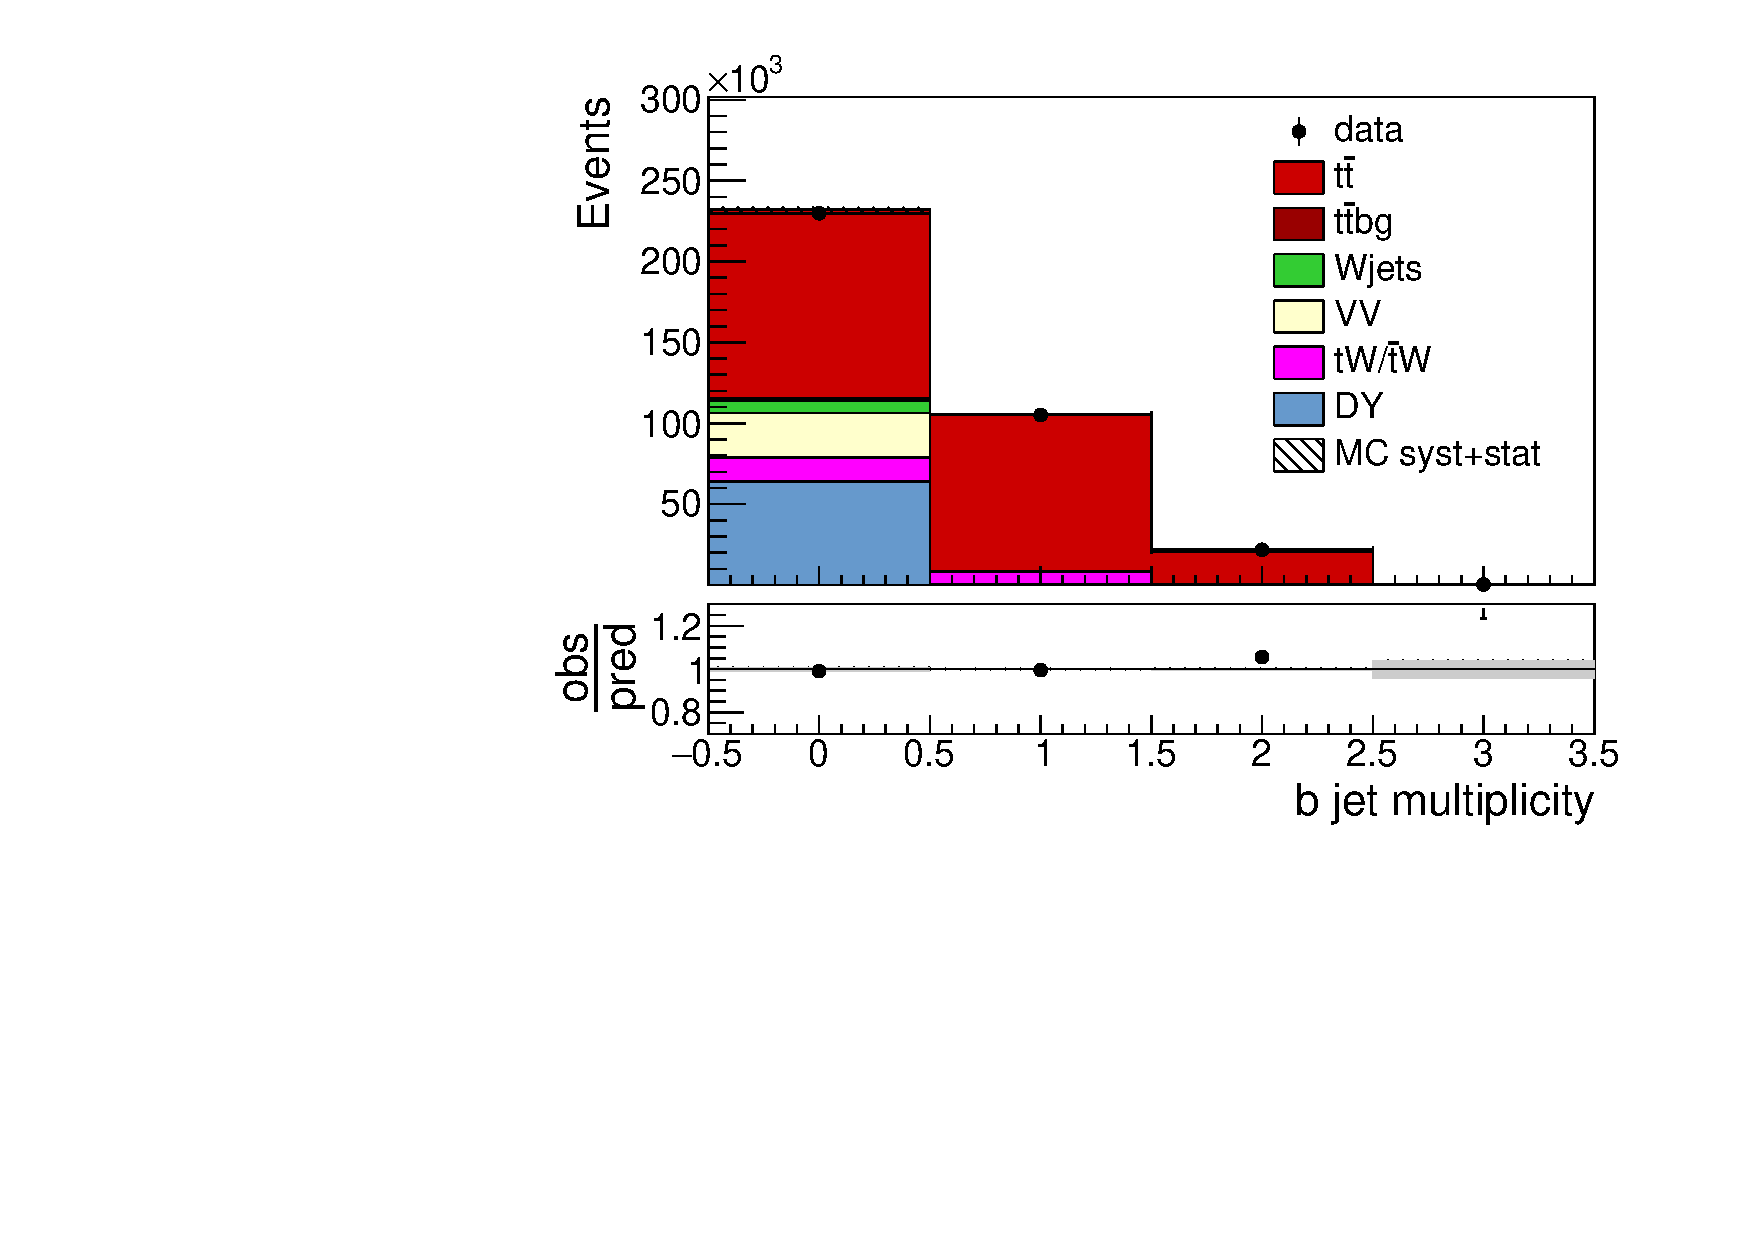
\includegraphics{SystematicUncerts/Figures/variationPlots/controlPlots/BTAGH/selected_b-jet_multi_step_8_BTAGH_down.pdf}}
    \resizebox{0.32 \textwidth}{!}{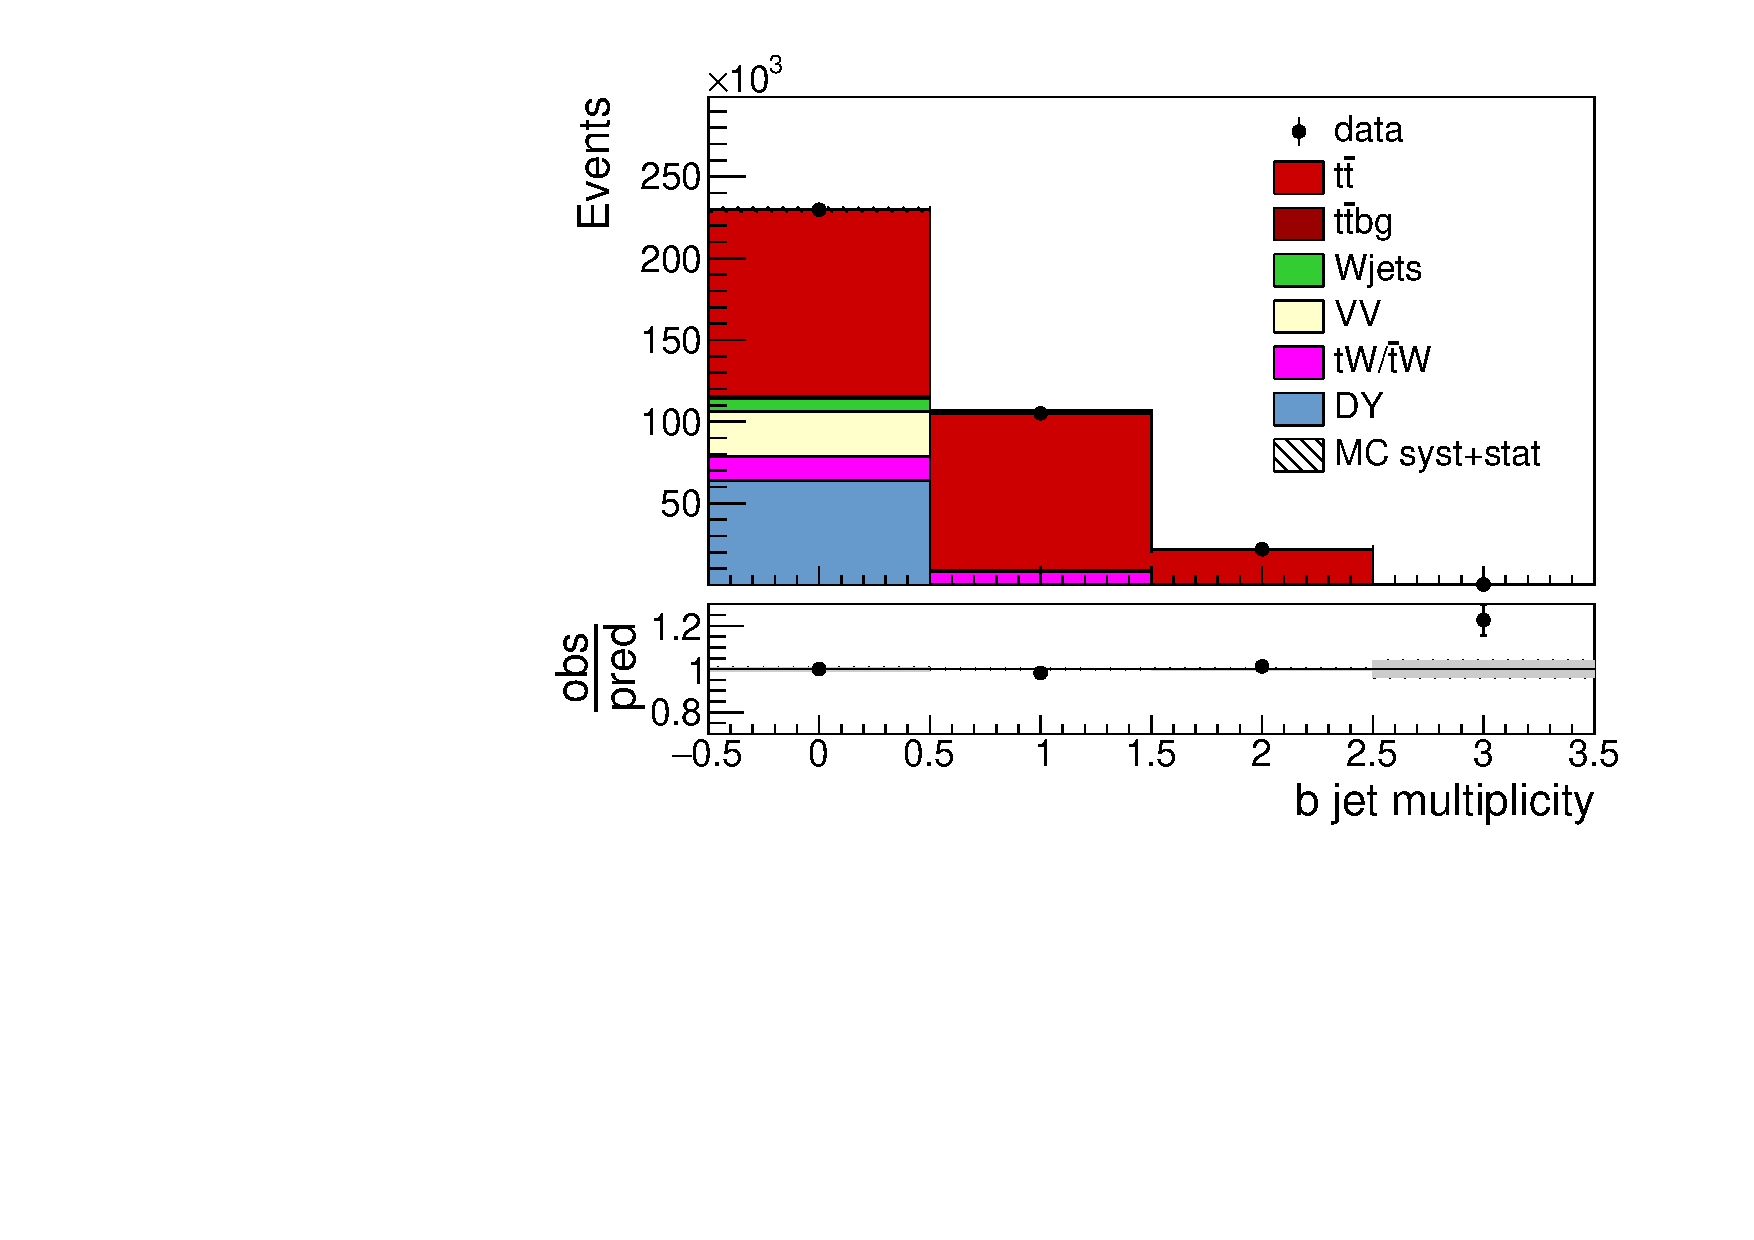
\includegraphics{SystematicUncerts/Figures/variationPlots/controlPlots/BTAGH/selected_b-jet_multi_step_8_nominal.pdf}}
    \resizebox{0.32 \textwidth}{!}{\includegraphics{SystematicUncerts/Figures/variationPlots/controlPlots/BTAGH/selected_b-jet_multi_step_8_BTAGH_up.pdf}}

\caption{Multiplicity of b-tagged jets in the \emu channel for the two systematic variations (left,right) and the nominal (middle) b-tagging efficiency.
The hatched bands correspond to the statistical uncertainty on the sum of the predicted yields. 
        The ratios of the event yield in data to the sum of the predicted yields are
        shown at the bottom of each plot. Here, the solid gray band
        represents the contribution of the statistical uncertainty.
  \label{fig:control_var_BTAGH}}
  \end{center}
\end{figure}


\subsection{Further Experimental Uncertainties}

The estimation of pile-up (see Section \todo{Link to reco}) in simulation is corrected according to the assumed number of collisions per bunch crossing in data. The number of additional collisions
in data is calculated for small time periods from the total inelastic proton proton cross section and the instantaneous luminosity in that time period.  
Events in simulation are reweighted depending on the number of primary vertices. To estimate the systematic uncertainty of this correction the total proton-proton cross section is changed
by $4.6 \; \%$ based on a measurement by the ATLAS collaboration \ref{Aaboud:2016mmw}. New eventweights are then estimated based on the changed value of the total proton-proton cross section.
The impact of these variations is shown in the distribution of the number of primary vertices per event as shown in Figure \ref{fig:control_var_PU}.
A mismatch between measured data and simulated events is visible in the nominal distribution, but as shown in the left figure, the systematic variations cover this discrapency.
This can lead to a fit result for the specific nuisance parameter tied to the systematic variation being different from one.

\begin{figure}[htbp!]
  \begin{center}
    \resizebox{0.32 \textwidth}{!}{\includegraphics{SystematicUncerts/Figures/variationPlots/controlPlots/PU/vertex_multiplicity_step_8_PU_down.pdf}}
    \resizebox{0.32 \textwidth}{!}{\includegraphics{SystematicUncerts/Figures/variationPlots/controlPlots/PU/vertex_multiplicity_step_8_nominal.pdf}}
    \resizebox{0.32 \textwidth}{!}{\includegraphics{SystematicUncerts/Figures/variationPlots/controlPlots/PU/vertex_multiplicity_step_8_PU_up.pdf}}
\caption{The number of primary vertices per event in the \emu channel for the two systematic variations (left,right) and the nominal (middle) pile-up corrections.
The hatched bands correspond to the statistical uncertainty on the sum of the predicted yields. 
        The ratios of the event yield in data to the sum of the predicted yields are
        shown at the bottom of each plot. Here, the solid gray band
        represents the contribution of the statistical uncertainty.
  \label{fig:control_var_PU}}
  \end{center}
\end{figure}


The integrated luminosity is determined by extrapolating the result of a measurement \todo{cite} of the instantaneous luminosity using special proton beam conditions (Van der Meer scan \ref{Zanetti:1357856}) to the full data taking period.
The uncertainty on the luminosity is determined in a dedicated analysis by both taking into account the uncertainty on the initial measurement itself as well as uncertainties
introduced in the extrapolation, mainly through changes in detector or beam conditions.
The systematic uncertainty on the luminosity is totally independent from the measurement of the \ttbar cross section and the other uncertainties described in this chapter.
It is not included as a nuisance parameter in the fit. It is directly applied to the final measurement of the \ttbar cross section by adding it in quadrature to the other uncertainties (see Equation \ref{eq:CaC})

\section{Theoretical Uncertainties}
\label{sec:theo_uncert}

The distributions used in the fit in this analysis are taken from simulation. In principle the physics model itself is not relevant, provided the simulation correctly predicts the event distribution for a given process.
The Standard Model reliably predicts the event distribution for the processes in this measurement especially for \ttbar production.
The simulation is based on assumptions for multiple parameters, some of which are based on the Standard Model. The uncertainties on the simulation are determined by the variation of these key parameters and they are
evaluated by repeating the simulation with changed parameters. The nominal simulation is then replaced with the systematically varied simulation to propagate the uncertainty to the final measurement.
The overall normalization of simulated \ttbar events is not changed with respect to the nominal sample, so the theoretical uncertainties described have a larger effect on the shape of the templates used
in the analysis than on the normalisation.

The \POWHEG simulation generates \ttbar events at NLO as described in Section \todo{Link}.
Additional particles radiated from the initial and final states are modelled in the parton shower, but the possible impact of these higher orders on the matrix element calculations is taken into account as an uncertainty.
Following convention \todo{cite smth., book from Klaus ?} the renormalization and factorisation scales are varied by the factors $2$ and $0.5$ resulting in a two-sided variation.
These variations are predicted to cover a possible change from inclusion of higher orders.
A uniform prior is used for the variation, with a value of unity between the $+1 \; \sigma$ and $-1 \; \sigma$ variations and zero everywhere else.
The impact of the matrix element scale variation is shown in Figure \ref{fig:control_var_TT_MESCALE} for the distribution of the number of jets for events with one b-tagged jet for events in the \emu channel.
These scale variations mostly affect the jets originating from particles simulated in the matrix element calculations, which often correspond to the three jets with the highest reconstructed $\pt$.
The $\pt$ of the jets is influenced by the scale and this change of $\pt$ propagates to the number of reconstructed jets due to the $\pt$ requirement in the selection of jets.

\begin{figure}[htbp!]
  \begin{center}
     \resizebox{0.32 \textwidth}{!}{\includegraphics{SystematicUncerts/Figures/variationPlots/controlPlots/TT_MESCALE/jet_multi_1x_b-jets_step_8_TT_MESCALE_down.pdf}}
    \resizebox{0.32 \textwidth}{!}{\includegraphics{SystematicUncerts/Figures/variationPlots/controlPlots/TT_MESCALE/jet_multi_1x_b-jets_step_8_nominal.pdf}}
    \resizebox{0.32 \textwidth}{!}{\includegraphics{SystematicUncerts/Figures/variationPlots/controlPlots/TT_MESCALE/jet_multi_1x_b-jets_step_8_TT_MESCALE_up.pdf}}
\caption{Number of additional jets for events with one b-tagged jet in the \emu channel for the two systematic variations (left, right) and the nominal \ttbar matrix element scale.
The hatched bands correspond to the statistical uncertainty on the sum of the predicted yields. 
        The ratios of the event yield in data to the sum of the predicted yields are
        shown at the bottom of each plot. Here, the solid gray band
        represents the contribution of the statistical uncertainty.
  \label{fig:control_var_TT_MESCALE}}
  \end{center}
\end{figure}

A similar uncertainty is applied to the scale of the parton shower calculations as modeled by \PYTHIA, split between the scale parameter impacting initial state radiation (ISR) and final state radiation (FSR). 
For the ISR scale the parameter is again varied by a factor of $2$ and $0.5$ respectively. The FSR scale parameter is varied by a factor of $\sqrt{2}$ or $\sqrt{0.5}$, following the recommendation
in Reference\cite{Skands:2014pea}. 
These uncertainties should also cover uncertainties on the detector response. Possible correlations between these theoretical uncertainties and  experimental uncertainties 
are taken into account by fitting all nuisance parameters simultaneously.
Figures \ref{fig:control_var_TT_ISRSCALE}
and \ref{fig:control_var_TT_FSRSCALE} show the variations to ISR and FSR respectively for the distribution of the number of additional jets for events with one b-tagged jet in the \emu channel.
Up to three jets can originate from particles generated in the matrix element calculations, so the impact of any changes in the parton shower scale are best seen in events with three or additional jets.
The plots also show a change in general normalisation because events migrate between the different categories for the number of b-tagged jets.

\begin{figure}[htbp!]
  \begin{center}
      \resizebox{0.32 \textwidth}{!}{\includegraphics{SystematicUncerts/Figures/variationPlots/controlPlots/TT_ISRSCALE/jet_multi_1x_b-jets_step_8_TT_ISRSCALE_down.pdf}}
    \resizebox{0.32 \textwidth}{!}{\includegraphics{SystematicUncerts/Figures/variationPlots/controlPlots/TT_ISRSCALE/jet_multi_1x_b-jets_step_8_nominal.pdf}}
    \resizebox{0.32 \textwidth}{!}{\includegraphics{SystematicUncerts/Figures/variationPlots/controlPlots/TT_ISRSCALE/jet_multi_1x_b-jets_step_8_TT_ISRSCALE_up.pdf}}
\caption{Number of additional jets for events with one b-tagged jet in the \emu channel for the two systematic variations (left, right) and the nominal ISR scale.
The hatched bands correspond to the statistical uncertainty on the sum of the predicted yields. 
        The ratios of the event yield in data to the sum of the predicted yields are
        shown at the bottom of each plot. Here, the solid gray band
        represents the contribution of the statistical uncertainty
  \label{fig:control_var_TT_ISRSCALE}}
  \end{center}
\end{figure}

\begin{figure}[htbp!]
  \begin{center}
      \resizebox{0.32 \textwidth}{!}{\includegraphics{SystematicUncerts/Figures/variationPlots/controlPlots/TT_FSRSCALE/jet_multi_1x_b-jets_step_8_TT_FSRSCALE_down.pdf}}
    \resizebox{0.32 \textwidth}{!}{\includegraphics{SystematicUncerts/Figures/variationPlots/controlPlots/TT_FSRSCALE/jet_multi_1x_b-jets_step_8_nominal.pdf}}
    \resizebox{0.32 \textwidth}{!}{\includegraphics{SystematicUncerts/Figures/variationPlots/controlPlots/TT_FSRSCALE/jet_multi_1x_b-jets_step_8_TT_FSRSCALE_up.pdf}}
\caption{Number of additional jets for events with one b-tagged jet in the \emu channel for the two systematic variations (left, right) and the nominal FSR scale.
The hatched bands correspond to the statistical uncertainty on the sum of the predicted yields. 
        The ratios of the event yield in data to the sum of the predicted yields are
        shown at the bottom of each plot. Here, the solid gray band
        represents the contribution of the statistical uncertainty
  \label{fig:control_var_TT_FSRSCALE}}
  \end{center}
\end{figure}


In order to avoid overlap between particles generated in \POWHEG and \PYTHIA the emissions generated in Powheg are dampened according to the parameter $h_{damp}$ by a factor of $h_{damp}^2 / (h_{damp}^2 + \pt^2)$.
To obtain the systematic variations $h_{damp}$ is varied within it's uncertainty of $h_{damp} = 1.58^{+0.66}_{-0.59} m_t$
as determined by measurements using data taken by CMS at a center of mass energy of 8 TeV \cite{CMS-PAS-TOP-16-021}.

The simulation of the underlying event is tuned to data measured by CMS \cite{CMS-PAS-TOP-16-021}. The uncertainty from that tuning is propagated to the simulation resulting in a two sided variation.

The dependence on the model of color reconnection used for the hadronization in \PYTHIA is evaluated by comparing the nominal simulation with three different models \cite{Argyropoulos:2014zoa,Christiansen:2015yqa}. This results in three one-sided variations.

Differential measurements of the \ttbar cross section \cite{CMS-PAS-TOP-16-011} have shown that the simulation does not fully model the \pt distribution of the top quarks.
This is likely due to higher order effects as shown by differential NNLO calculations \ref{PhysRevLett.116.082003}. In order to model that disagreement a one-sided variation is introduced where simulated events are reweighted according to the \pt of the top quark with a factor of $\sqrt{SF(t)SF(\bar{t})}$ with $SF(\pT)=e^{0.0615-0.0005\cdot \pT}$.
This reweighting corrects the simulation to the measurement.

The uncertainty from the choice of PDF is evaluated using the variations provided by the CT14 PDF set \cite{Dulat:2015mca}. Uncorrelated variations are constructed from the central CT14 result using 56 eigenvectors resulting in 28 two-sided variations.
The variations are used at the $68 \;\%$ confidence level. Each of the variations is treated as a separate nuisance parameter.


The branching ratio of B mesons in \PYTHIA does not exactly agree with the values from the PDG  \todo{cite}. Especially a semi-leptonic decay of the B meson causes a different detector response compared to a hadronic decay,
which propagates to a differently reconstructed b-jet introducing an uncertainty.
This uncertainty is modelled by reweighting the events so that the branching ratio in simulation agrees with the one in the PDG and the uncertainties on the prediction serve as systematic
variations. These variations are given a uniform nuisance parameter.

The momentum transfer from the b-quark to the B meson (fragmentation function) is controlled by \PYTHIA and can influence the kinematics of the reconstructed b-jet. 
The default modelling uses the Bowler-Lund model \ref{Bowler1981} with the parameter of $StringZ:rFactB = 0.855$ \ref{Skands:2014pea,CMS-PAS-TOP-16-021}.
The respective parameter is tuned to LEP data and its uncertainty is used as a systematic variation, resulting in $StringZ:rFactB = 0.855^{+0.224}_{-0.157}$.
The Peterson fragmentation function \ref{PhysRevD.27.105} is used as an additional one-sided variation. 



%!TEX root = ../thesis.tex
%*******************************************************************************
%****************************** Second Chapter *********************************
%*******************************************************************************

\chapter{Introduction}






% ********************************** Back Matter *******************************
% Backmatter should be commented out, if you are using appendices after References
%\backmatter

% ********************************** Bibliography ******************************
\begin{spacing}{0.9}

% To use the conventional natbib style referencing
% Bibliography style previews: http://nodonn.tipido.net/bibstyle.php
% Reference styles: http://sites.stat.psu.edu/~surajit/present/bib.htm

\bibliographystyle{apalike}
%\bibliographystyle{unsrt} % Use for unsorted references  
%\bibliographystyle{plainnat} % use this to have URLs listed in References
\cleardoublepage
\bibliography{References/references} % Path to your References.bib file


% If you would like to use BibLaTeX for your references, pass `custombib' as
% an option in the document class. The location of 'reference.bib' should be
% specified in the preamble.tex file in the custombib section.
% Comment out the lines related to natbib above and uncomment the following line.

%\printbibliography[heading=bibintoc, title={References}]


\end{spacing}

% ********************************** Appendices ********************************

\begin{appendices} % Using appendices environment for more functunality

%!TEX root = ../thesis.tex
% ******************************* Thesis Appendix A ****************************
\chapter{Detailed breakdown of systematic uncertainties} 
\label{app:uncert}

\begin{longtable}{ l | c | c | c }%[htbp!]
%\center
\caption{Extracted cross sections with detailed
  list of uncertainties. Besides the contribution to the total
  uncertainty in \%, the fitted value of the nuisance parameter (pull), as well as the ratio of the estimated
  uncertainty over the uncertainty from a 1 $\sigma$ variation, called
  constr/$\sigma$, are shown. 
  \label{tab:lh_res_eightfull}}\\
\hline
Name & Pull & Constr / $\sigma$ & Contribution [\%] \\ 
\hline
\endfirsthead
\hline
Name & Pull & Constr / $\sigma$ & Contribution [\%] \\ 
\hline
\endhead
B-tag & 0.617 & 0.49 & ${0.456}$ \\
Mistag & 0.413 & 0.96 & ${0.129}$ \\
DY ME scale & -0.583 & 0.44 & ${0.118}$ \\
Electron energy resolution & -0.076 & 0.91 & ${-0.007}$ \\
Electron energy scale & -1.271 & 0.63 & ${-0.015}$ \\
Electron ID & 0.291 & 0.6 & ${-1.907}$ \\
Jet energy resolution & 1.096 & 0.81 & ${-0.008}$ \\
JES: MPF & 0.101 & 0.66 & ${0.002}$ \\
JES: Absolute Scale & -0.053 & 0.77 & ${0.019}$ \\
JES: Absolute Stat & 0.266 & 0.83 & ${-0.039}$ \\
JES\_Fragmentation & 0.203 & 0.63 & ${-0.038}$ \\
JES: Pileup Data/MC & -0.265 & 0.89 & ${-0.063}$ \\
JES: Pileup $p_T$ BB & 0.166 & 0.75 & ${-0.093}$ \\
JES\_PileUpPtEC1 & -0.12 & 0.65 & ${-0.046}$ \\
JES\_PileUpPtRef & 0.28 & 0.56 & ${-0.084}$ \\
JES\_RelativeBal & -0.709 & 0.52 & ${0.143}$ \\
JES: Intercalibration & 0.068 & 0.66 & ${-0.001}$ \\
JES: Relative JER EC1 & -0.074 & 1.03 & ${0.008}$ \\
JES: Relative $p_T$ BB & -0.025 & 0.87 & ${0.019}$ \\
JES: Relative $p_T$ EC1 & -0.012 & 0.91 & ${-0.049}$ \\
JES\_RelativeStatEC & 0.296 & 0.73 & ${-0.026}$ \\
JES\_RelativeStatFSR & -0.085 & 1.07 & ${0.033}$ \\
JES: Single pion ECAL & 0.264 & 0.6 & ${-0.060}$ \\
JES: Single pion HCAL & 0.171 & 0.63 & ${-0.026}$ \\
JES\_TimePtEta & 0.255 & 0.68 & ${-0.019}$ \\
Muon energy scale & 0.114 & 0.99 & ${0.043}$ \\
Muon ID & -0.343 & 0.84 & ${-2.021}$ \\
Pile-up & 0.511 & 0.82 & ${0.312}$ \\
top mass & 0 & 0 & ${0.000}$ \\
Top $p_{T}$ & 1 & 0.74 & ${-0.001}$ \\
Trigger & -0.022 & 0.99 & ${-0.645}$ \\
B-hadron BR & 0.093 & 0.72 & ${0.075}$ \\
TT\_CRERD & 0 & 0.69 & ${0.000}$ \\
TT\_CRGLUON & 0.184 & 0.17 & ${0.006}$ \\
TT\_CRQCD & 0.105 & 0.12 & ${0.139}$ \\
fragm. Peterson & 0.521 & 0.41 & ${0.302}$ \\
fragmentation & -0.768 & 0.58 & ${-0.694}$ \\
$t\bar{t}$/tW FSR scale & -0.201 & 0.17 & ${0.560}$ \\
NLO generator & 0 & 0 & ${0.000}$ \\
$t\bar{t}$/tW ISR scale & 0.111 & 0.18 & ${-0.305}$ \\
ME/PS matching & -0.138 & 0.2 & ${0.148}$ \\
$t\bar{t}$ ME scale & 1 & 0.32 & ${0.000}$ \\
UE tune & 0.163 & 0.26 & ${0.180}$ \\
PDF10 & -0.065 & 0.84 & ${0.367}$ \\
PDF11 & -0.003 & 0.86 & ${0.139}$ \\
PDF12 & 0.022 & 0.86 & ${-0.209}$ \\
PDF13 & 0.21 & 0.85 & ${0.155}$ \\
PDF14 & 0.06 & 0.87 & ${-0.082}$ \\
PDF15 & 0.061 & 0.83 & ${-0.051}$ \\
PDF16 & 0.004 & 0.86 & ${0.061}$ \\
PDF17 & -0.043 & 0.85 & ${-0.150}$ \\
PDF18 & -0.228 & 0.85 & ${0.021}$ \\
PDF19 & -0.106 & 0.82 & ${0.257}$ \\
PDF1 & -0.018 & 0.88 & ${-0.037}$ \\
PDF20 & 0.002 & 0.83 & ${0.098}$ \\
PDF21 & -0.115 & 0.86 & ${-0.173}$ \\
PDF22 & -0.239 & 0.85 & ${-0.223}$ \\
PDF23 & 0.096 & 0.76 & ${-0.008}$ \\
PDF24 & 0.104 & 0.87 & ${0.137}$ \\
PDF25 & -0.083 & 0.83 & ${-0.020}$ \\
PDF26 & 0.013 & 0.83 & ${0.021}$ \\
PDF27 & -0.045 & 0.88 & ${0.092}$ \\
PDF28 & 0.035 & 0.85 & ${-0.011}$ \\
PDF2 & -0.241 & 0.97 & ${-0.047}$ \\
PDF3 & -0.005 & 0.86 & ${0.147}$ \\
PDF4 & -0.092 & 0.92 & ${0.071}$ \\
PDF5 & 0.085 & 0.8 & ${-0.329}$ \\
PDF6 & -0.006 & 0.87 & ${0.109}$ \\
PDF7 & 0.16 & 0.78 & ${-0.385}$ \\
PDF8 & 0.046 & 0.85 & ${-0.026}$ \\
PDF9 & -0.084 & 0.85 & ${-0.014}$ \\
JES: Flavor response & -0.335 & 0.63 & ${-0.076}$ \\
tW background & -0.422 & 0.46 & ${-0.815}$ \\
Diboson background & 0.849 & 0.78 & ${0.206}$ \\
W+jets background & -0.905 & 0.83 & ${0.036}$ \\
$t\bar{t}$ background & 0.102 & 0.98 & ${-0.084}$ \\
DY background (0 b-jets) & -0.045 & 0.36 & ${0.430}$ \\
DY background (1 b-jets) & -0.429 & 0.22 & ${0.172}$ \\
DY background (2 b-jets) & -0.643 & 0.78 & ${-0.014}$ \\
Stat &  &  & ${0.252}$ \\
Total vis &  &  & $\pm^{2.648}_{2.549}$ \\ \hline
$\sigma_{t\bar{t}}$(13 TeV) vis &   &   & 28.1033 pb \\ \hline
$t\bar{t}$/tW ISR scale (extr) &  &  & $\mp^{0.146}_{0.105}$ \\
$t\bar{t}$/tW FSR scale (extr) &  &  & $\pm^{0.084}_{0.065}$ \\
$t\bar{t}$ ME scale (extr) &  &  & $\mp^{0.392}_{0.000}$ \\
UE tune (extr) &  &  & $\mp^{0.188}_{0.053}$ \\
PDF (extr) &  &  & $\pm^{0.818}_{0.588}$ \\
Top $p_{T}$ (extr) &  &  & $\pm^{0.000}_{0.446}$ \\ \hline
Total &  &  & $\pm^{2.810}_{2.654}$ \\ \hline
$\sigma_{t\bar{t}}$(13 TeV) &   &   & 819.95 pb \\ \\ \hline \hline

\end{longtable}
%!TEX root = ../thesis.tex
% ******************************* Thesis Appendix B ********************************

\chapter{List of publications}

\begin{itemize}

\item Measurement of the top quark pair production cross section at 13 TeV with the CMS detector, \\
T. Arndt, PoS TOP2015 (2016) 026

\item Measurement of the top quark pair production cross section using e$\mu$ events in proton-proton
collisions at $\sqrt{s}= 13 \TeV$ with the CMS detector, \\
CMS Collaboration, Eur.Phys.J. C77 (2017) 172, DOI: 10.1140/epjc/s10052-017-4718-8

\item Measurement of the top quark pair production cross section in proton-proton collisions at $\sqrt{s}= 13 \TeV$ with the CMS detector, \\
CMS Collaboration, Phys. Rev. Lett. 116 (2016) 052002, DOI: 10.1103/PhysRevLett.116.052002

\item Measurement of normalized differential tt cross sections in the dilepton channel from pp
collisions at $\sqrt{s}= 13 \TeV$, \\
CMS Collaboration, JHEP 1704 (2017) 060, DOI: 10.1007/JHEP04(2018)060

\item Search for $\ttbar\mathrm{H}$ production in the $\mathrm{H}\rightarrow\mathrm{b}\bar{\mathrm{b}}$ decay channel with leptonic \ttbar decays in proton-proton
collisions at $\sqrt{s}= 13 \TeV$, \\
CMS Collaboration, Preliminary publication, April 2018, CMS-PAS-HIG-17-026

\item Search for $\ttbar\mathrm{H}$ production in the $\mathrm{H}\rightarrow\mathrm{b}\bar{\mathrm{b}}$ decay channel with $\sqrt{s}= 13 \TeV$ pp collisions at the CMS
experiment,\\
CMS Collaboration, Preliminary publication, March 2016, CMS-PAS-HIG-16-004

\item First measurement of the differential cross section for \ttbar production in the dilepton final
state at $\sqrt{s}= 13 \TeV$, \\
CMS Collaboration, Preliminary publication, August 2015, CMS-PAS-TOP-15-010

\end{itemize}




\end{appendices}

% *************************************** Index ********************************
\printthesisindex % If index is present

\end{document}
